%%%%%%%%%%%%%%
%% Run LaTeX on this file several times to get Table of Contents,
%% cross-references, and citations.

%% If you have font problems, you may edit the w-bookps.sty file
%% to customize the font names to match those on your system.

%% w-bksamp.tex. Current Version: Feb 16, 2012
%%%%%%%%%%%%%%%%%%%%%%%%%%%%%%%%%%%%%%%%%%%%%%%%%%%%%%%%%%%%%%%%
%
%  Sample file for
%  Wiley Book Style, Design No.: SD 001B, 7x10
%  Wiley Book Style, Design No.: SD 004B, 6x9
%
%
%  Prepared by Amy Hendrickson, TeXnology Inc.
%  http://www.texnology.com
%%%%%%%%%%%%%%%%%%%%%%%%%%%%%%%%%%%%%%%%%%%%%%%%%%%%%%%%%%%%%%%%

%%%%%%%%%%%%%
% 7x10
%\documentclass{wileySev}

% 6x9
\documentclass{wileySix}

\usepackage{graphicx}

\UseRawInputEncoding

%%%%%%%
%% for times math: However, this package disables bold math (!)
%% \mathbf{x} will still work, but you will not have bold math
%% in section heads or chapter titles. If you don't use math
%% in those environments, mathptmx might be a good choice.

% \usepackage{mathptmx}

% For PostScript text
\usepackage{w-bookps}

%%%%%%%%%%%%%%%%%%%%%%%%%%%%%%%%%%%%%%%%%%%%%%%%%%%%%%%%%%%%%%%%
%% Other packages you might want to use:

% for chapter bibliography made with BibTeX
% \usepackage{chapterbib}

% for multiple indices
% \usepackage{multind}

% for answers to problems
% \usepackage{answers}

%%%%%%%%%%%%%%%%%%%%%%%%%%%%%%
%% Change options here if you want:
%%
%% How many levels of section head would you like numbered?
%% 0= no section numbers, 1= section, 2= subsection, 3= subsubsection
%%==>>
\setcounter{secnumdepth}{3}

%% How many levels of section head would you like to appear in the
%% Table of Contents?
%% 0= chapter titles, 1= section titles, 2= subsection titles, 
%% 3= subsubsection titles.
%%==>>
\setcounter{tocdepth}{2}

%% Cropmarks? good for final page makeup
%% \docropmarks

%%%%%%%%%%%%%%%%%%%%%%%%%%%%%%
%
% DRAFT
%
% Uncomment to get double spacing between lines, current date and time
% printed at bottom of page.
% \draft
% (If you want to keep tables from becoming double spaced also uncomment
% this):
% \renewcommand{\arraystretch}{0.6}
%%%%%%%%%%%%%%%%%%%%%%%%%%%%%%

%%%%%%% Demo of section head containing sample macro:
%% To get a macro to expand correctly in a section head, with upper and
%% lower case math, put the definition and set the box 
%% before \begin{document}, so that when it appears in the 
%% table of contents it will also work:

\newcommand{\VT}[1]{\ensuremath{{V_{T#1}}}}

%% use a box to expand the macro before we put it into the section head:

\newbox\sectsavebox
\setbox\sectsavebox=\hbox{\boldmath\VT{xyz}}

%%%%%%%%%%%%%%%%% End Demo


\begin{document}


\booktitle{Belajar Latex}
\subtitle{Cerdas Pahami Latex}

\authors{Rolly M. Awangga\\
\affil{Politeknik Pos Indonesia}
}

\offprintinfo{Survey Methodology, Second Edition}{Robert M. Groves}

%% Can use \\ if title, and edition are too wide, ie,
%% \offprintinfo{Survey Methodology,\\ Second Edition}{Robert M. Groves}

%%%%%%%%%%%%%%%%%%%%%%%%%%%%%%
%% 
\halftitlepage

\titlepage


\begin{copyrightpage}{2007}
Survey Methodology / Robert M. Groves . . . [et al.].
\       p. cm.---(Wiley series in survey methodology)
\    ``Wiley-Interscience."
\    Includes bibliographical references and index.
\    ISBN 0-471-48348-6 (pbk.)
\    1. Surveys---Methodology.  2. Social 
\  sciences---Research---Statistical methods.  I. Groves, Robert M.  II. %
Series.\\

HA31.2.S873 2007
001.4'33---dc22                                             2004044064
\end{copyrightpage}

\dedication{To my parents}

\begin{contributors}
\name{Masayki Abe,} Fujitsu Laboratories Ltd., Fujitsu Limited, Atsugi,
Japan

\name{L. A. Akers,} Center for Solid State Electronics Research, Arizona
State University, Tempe, Arizona

\name{G. H. Bernstein,} Department of Electrical and
Computer Engineering, University of Notre Dame, Notre Dame, South Bend, 
Indiana; formerly of
Center for Solid State Electronics Research, Arizona
State University, Tempe, Arizona 
\end{contributors}

\contentsinbrief
\tableofcontents
\listoffigures
\listoftables


\begin{foreword}
This is the foreword to the book.
\end{foreword}

\begin{preface}
This is an example preface.
This is an example preface.
This is an example preface.
This is an example preface.

\prefaceauthor{R. K. Watts}
\where{Durham, North Carolina\\
September, 2007}

\end{preface}


\begin{acknowledgments}
From Dr.~Jay Young, consultant from Silver Spring, Maryland, I received
the initial push to even consider writing this book. Jay was a constant
``peer reader'' and very welcome advisor durying this year-long process.


To all these wonderful people I owe a deep sense of gratitude especially now
that this project has been completed.
\authorinitials{G. T. S.}
\end{acknowledgments}

\begin{acronyms}
\acro{ACGIH}{American Conference of Governmental Industrial Hygienists}
\acro{AEC}{Atomic Energy Commission}
\acro{OSHA}{Occupational Health and Safety Commission}
\acro{SAMA}{Scientific Apparatus Makers Association}
\end{acronyms}

\begin{glossary}
\term{NormGibbs}Draw a sample from a posterior distribution
of data with an unknown mean and variance using Gibbs sampling.

\term{pNull}Test a one sided hypothesis from a numberically
specified posterior CDF or from a sample from the posterior

\term{sintegral}A numerical integration using Simpson's rule
\end{glossary}

\begin{symbols}
\term{A}Amplitude

\term{\hbox{\&}}Propositional logic symbol 

\term{a}Filter Coefficient

\bigskip

\term{\mathcal{B}}Number of Beats
\end{symbols}

\begin{introduction}

%% optional, but if you want to list author:

\introauthor{Catherine Clark, PhD.}
{Harvard School of Public Health\\
Boston, MA, USA}

The era of modern \index{microelectronics}\index{microelectronics!modern} 
began in 1958 with the invention of the
integrated circuit by J.~S.~Kilby
 of Texas Instruments \cite{kilby}.
His first chip is shown in Fig.~I. For comparison,
Fig.~I.2 shows a modern microprocessor chip, \cite{beren}.


This is the introduction.
This is the introduction.
This is the introduction.
This is the introduction.
This is the introduction.
This is the introduction.

\begin{equation}
ABC {\cal DEF} \alpha\beta\Gamma\Delta\sum^{abc}_{def}
\end{equation}


\begin{chapreferences}{3.}
\bibitem{zkilby}J. S. Kilby,
``Invention of the Integrated Circuit,'' {\it IEEE Trans. Electron Devices,}
{\bf ED-23,} 648 (1976).

\bibitem{zhamming}R. W. Hamming,
                 {\it Numerical Methods for Scientists and 
                 Engineers}, Chapter N-1, McGraw-Hill, 
                 New York, 1962.

\bibitem{zHu}J. Lee, K. Mayaram, and C. Hu, ``A Theoretical
               Study of Gate/Drain Offset in LDD MOSFETs''
                     {\it IEEE Electron Device Lett.,} {\bf EDL-7}(3). 152 
                     (1986).
\end{chapreferences}
\end{introduction}


\part[Submicron Semiconductor Manufacture]
{Submicron Semiconductor\\ Manufacture}


\chapter[The Submicrometer Silicon MOSFET]
{The Submicrometer\\ Silicon MOSFET}


\prologue{The sheer volumne of answers can often stifle insight...The purpose
of computing\index{computing!the purpose} is insight, not numbers.}
{Hamming \cite{hamming}}


\section{Here is a normal section}
Here is some text.

\subsection{This is the subsection}
Here is some normal text.
Here is some normal text.
Here is some normal text.
Here is some normal text.
Here is some normal text.
Here is some normal text.
Here is some normal text.
Here is some normal text.
Here is some normal text.
Here is some normal text.
Here is some normal text.


\subsubsection{This is the subsubsection}
Here is some text after the subsubsection.
Here is some text after the subsubsection.
Here is some text after the subsubsection.
Here is some text after the subsubsection.

\paragraph{This is the paragraph}
Here is some normal text.
Here is some normal text.
Here is some normal text.
Here is some normal text.

\section{Tips On Special Section Heads}
Here are some things you can do for a special
section head.

\section[This Version of Section Head will be sent Contents]
{Break Long Section heads\\ with double backslash}
Here is some normal text.
Here is some normal text.
Here is some normal text.

 \section[This show how to explicitly break lines
\string\hfill\string\break\space in Table of Contents]
{Here is a Section Title}
See this section head for information on how to explicitly break lines in
table of contents.

\section{How to get \lowercase{lower case} in section head: \lowercase{$p$}$H$}
Here is some normal text.
Here is some normal text.
Here is some normal text.

\section{How to use a macro that has both upper and lower case parts: 
\copy\sectsavebox}
See the top of this file where the definition and box were set.

%% Sending different version of section to running head, 
%% so that the size of math is correct in running head:
\markright{Sample macro \VT{\lowercase{xyz}} sent to running head}

\section{Equation}

For optimal vertical spacing, no blank lines before or after
equations
\begin{equation}
\alpha\beta\Gamma\Delta
\end{equation}
as you see here.


\chapter{First Edited Book Sample Chapter Title}
\chapterauthors{G. Alvarez and R. K. Watts
\chapteraffil{Carnegie Mellon University, Pittsburgh, Pennsylvania}
}

\section{Here is a normal section}
Here is some text.


\chapter{Second Edited Book Sample Chapter Title}
\chapterauthors{George Smeal, Ph.D.\affilmark{1}, Sally Smith,
M.D.\affilmark{2} and Stanley Kubrick\affilmark{1}
\chapteraffil{\affilmark{1}AT\&T Bell Laboratories
Murray Hill, New Jersey\\
\affilmark{2}Harvard Medical School,
Boston, Massachusetts}
}

\section{Sample Section}
Here is some sample text.

\newpage

\section{Example, Figure and Tables}
\vskip6pt
\begin{example}[Optional Example Name]
Use Black's law [Equation (6.3)] to estimate the reduction in useful product
life if a metal line is initially run at 55$^\circ$C at a maximum line
current density.
\end{example}




\begin{figure}[ht]
illustration here
%\centerline{\includegraphics[width=.5\textwidth]{filename}}
\caption{Short figure caption.}
\end{figure}

\begin{figure}[ht]
\vskip2pt
\caption{Oscillograph for  memory address access operations,
showing 500 ps
address access time and superimposed signals
of address access in 1 kbit
memory plane.}
\end{figure}

\begin{table}[ht]
\caption{Small Table}
\centering
\begin{tabular}{cccc}
\hline
one&two&three&four\\
\hline
C&D&E&F\\
\hline
\end{tabular}
\end{table}

\begin{table}[ht]
\caption{Effects of the two types of $\alpha\beta\sum^A_B$ scaling proposed by Dennard \newline
and
co-workers$^{a,b}$}
\begin{tabular*}{\textwidth}{@{\extracolsep{\fill}}lcc}
\hline
Parameter& $\kappa$ Scaling & $\kappa$, $\lambda$ Scaling\cr
\hline
Dimension&$\kappa^{-1}$&$\lambda^{-1}$\cr
Voltage&$\kappa^{-1}$&$\kappa^{-1}$\cr
Currant&$\kappa^{-1}$&$\lambda/\kappa^{2}$\cr
Dopant Concentration&$\kappa$&$\lambda^2/\kappa$\cr
\hline
\end{tabular*}
\begin{tablenotes}
$^a$Refs.~19 and 20.

$^b\kappa, \lambda>1$.
\end{tablenotes}
\end{table}

\subsection{Side by Side Tables and Figures}

\begin{figure}[ht]
\sidebyside{
Space for figure...
\caption{This caption will go on the left side of
the page. It is the initial caption of two side-by-side captions.}
}
{
Space for second figure...
\caption{This caption will go on the right side of
the page. It is the second of two side-by-side captions.}
}
\end{figure}


The command \verb+\sidebyside{}{}+ works similarly for tables:

 \begin{table}[ht]
 \sidebyside{
\caption{Table Caption} 
\begin{tabular}{cccc}
one&two&three&four\\
a &little&sample&table
\end{tabular}
}
 {
\caption{Table Caption}
\begin{tabular}{cccc}
A&B&C&D\\
a &second little& sample&table
\end{tabular}
}
 \end{table}


When using \verb+\sidebyside+, one must
use the cross referencing command \verb+\label{}+ after and  {\it outside} 
 of \verb+\caption{}+:

\begin{verbatim}
 \begin{table} 
 \sidebyside{\caption{Table Caption}\label{tab1}
 first table}
 {\caption{Table Caption}\label{tab2} second table}
 \end{table}
\end{verbatim}
 or,
\begin{verbatim}
 \begin{figure} 
 \sidebyside{\vskip<dimen>\caption{fig caption}\label{fig1}}
 {\vskip<dimen>\caption{fig caption}\label{fig2}}
 \end{figure}
\end{verbatim}





\section{Algorithm}
This is a sample algorithm.

\begin{algorithm}
{\bf state\_transition algorithm} $\{$
\        for each neuron $j\in\{0,1,\ldots,M-1\}$
\        $\{$   
\            calculate the weighted sum $S_j$ using Eq. (6);
\            if ($S_j>t_j$)
\                    $\{$turn ON neuron; $Y_1=+1\}$   
\            else if ($S_j<t_j$)
\                    $\{$turn OFF neuron; $Y_1=-1\}$   
\            else
\                    $\{$no change in neuron state; $y_j$ remains %
unchanged;$\}$ 
\        $\}$   
$\}$   
\end{algorithm}

Here is some normal text.
Here is some normal text.
Here is some normal text.
Here is some normal text.
Here is some normal text.
Here is some normal text.
Here is some normal text.
Here is some normal text.
Here is some normal text.
Here is some normal text.
Here is some normal text.
Here is some normal text.
Here is some normal text.
Here is some normal text.


\begin{quote}
This is a sample of extract or quotation.
This is a sample of extract or quotation.
This is a sample of extract or quotation.
\end{quote}

\begin{enumerate}
\item
This is the first item in the numbered list.

\item
This is the second item in the numbered list.
This is the second item in the numbered list.
This is the second item in the numbered list.
\end{enumerate}

\begin{itemize}
\item
This is the first item in the itemized list.

\item
This is the first item in the itemized list.
This is the first item in the itemized list.
This is the first item in the itemized list.
\end{itemize}

\begin{itemize}
\item[]
This is the first item in the itemized list.

\item[]
This is the first item in the itemized list.
This is the first item in the itemized list.
This is the first item in the itemized list.
\end{itemize}

\begin{problems}
\prob
For Hooker's data, Problem 1.2, use the Box and Cox and Atkinson procedures to determine a appropriate transformation of PRES
in the regression of PRES on TEMP. find $\hat\lambda$, $\tilde\lambda$,
the score test, and the added variable plot for the score. 
Summarize the results.

\prob
The following data were collected in a study of the effect of dissolved sulfur
on the surface tension of liquid copper (Baes and Killogg, 1953).

{\centering
\vskip6pt
\begin{tabular}{rlcc}
\hline
&&\multicolumn2c{$Y$= Decrease in Surface Tension}\\
\multicolumn2c{$x$ = Weight \% sulfur}
&\multicolumn2c{(dynes/cm), two Replicates}\\
\hline
0.&034&301&316\\
0.&093&430&422\\
0.&30&593&586\\
\hline
\end{tabular}
\vskip6pt
}


\subprob
Find the transformations of $X$ and $Y$ sot that in the transformed scale 
the regression is linear.

\subprob
Assuming that $X$ is transformed to $\ln(X)$, which choice of $Y$ gives 
better results,
$Y$ or $\ln(Y)$? (Sclove, 1972).

\sidebysidesubprob{In the case of $\alpha_1$?}{In the case of $\alpha_2$?}

\prob
Examine the Longley data, Problem 3.3, for applicability of assumptions of the
linear model.

\sidebysideprob{In the case of $\Gamma_1$?}{In the case of $\Gamma_2$?}

\end{problems}


\begin{exercises}
\exer
For Hooker's data, Exercise 1.2, use the Box and Cox and Atkinson procedures to determine a appropriate transformation of PRES
in the regression of PRES on TEMP. find $\hat\lambda$, $\tilde\lambda$,
the score test, and the added variable plot for the score. 
Summarize the results.

\exer
The following data were collected in a study of the effect of dissolved sulfur
on the surface tension of liquid copper (Baes and Killogg, 1953).

{\centering
\vskip6pt
\begin{tabular}{rlcc}
\hline
&&\multicolumn2c{$Y$= Decrease in Surface Tension}\\
\multicolumn2c{$x$ = Weight \% sulfur}
&\multicolumn2c{(dynes/cm), two Replicates}\\
\hline
0.&034&301&316\\
0.&093&430&422\\
0.&30&593&586\\
\hline
\end{tabular}
\vskip6pt
}


\subexer
Find the transformations of $X$ and $Y$ sot that in the transformed scale 
the regression is linear.

\subexer
Assuming that $X$ is transformed to $\ln(X)$, which choice of $Y$ gives 
better results,
$Y$ or $\ln(Y)$? (Sclove, 1972).

\sidebysidesubexer{In the case of $\Delta_1$?}{In the case of $\Delta_2$?}

\exer
Examine the Longley data, Problem 3.3, for applicability of assumptions of the
linear model.

\sidebysideexer{In the case of $\Gamma_1$?}{In the case of $\Gamma_2$?}

\end{exercises}


\section{Summary}
This is a summary of this chapter.
Here are some references: \cite{xkilby}, \cite{xberen}.

\begin{chapreferences}{5.}
\bibitem{xkilby}J. S. Kilby,
``Invention of the Integrated Circuit,'' {\it IEEE Trans. Electron Devices,}
{\bf ED-23,} 648 (1976).


\bibitem{xhamming}R. W. Hamming,
                 {\it Numerical Methods for Scientists and 
                 Engineers}, Chapter N-1, McGraw-Hill, 
                 New York, 1962.

\bibitem{xHu}J. Lee, K. Mayaram, and C. Hu, ``A Theoretical
               Study of Gate/Drain Offset in LDD MOSFETs''
                     {\it IEEE Electron Device Lett.,} {\bf EDL-7}(3). 152 
                     (1986).

\bibitem{xberen}A. Berenbaum, 
B. W. Colbry, D.R. Ditzel, R. D Freeman, and 
K.J. O'Connor, ``A Pipelined 32b Microprocessor with 13 kb of Cache Memory,''
{it Int. Solid State Circuit Conf., Dig. Tech. Pap.,} p. 34 (1987).
\end{chapreferences}


\chapappendix{This is the Chapter Appendix Title}
This is an appendix with a title.
\begin{equation}
\alpha\beta\Gamma\Delta
\end{equation}



\begin{figure}[ht]
\caption{This is an appendix figure caption.}
\end{figure}

\begin{table}[ht]
\caption{This is an appendix table caption}
\centering
\let\hline\savehline
\begin{tabular}{@{\vrule height 11pt depth 4pt width0pt}|l|p{.65\textwidth}|c}
\hline
{\bf Date} & \multicolumn1{c|}{\bf Event} \\
\hline \hline
1867 & Maxwell speculated the existence of electromagnetic waves.\\
1887 & Hertz showed the existence of electromagnetic waves. \\
1890 & Branly developed technique for detecting radio waves. \\
1896 & Marconi demonstrated wireless telegraph. \\
1897 & Marconi patented wireless telegraph.  \\
1898 & Marconi awarded patent for tuned communication. \\
1898 & Wireless telegraphic connection between England and France established. \\
\hline
\end{tabular}
\end{table}


\chapappendix{}
This is a Chapter Appendix without a title.

Here is a math test to show the difference between using Computer Modern
math fonts and MathTimes math fonts. When MathTimes math fonts are used
the letters in an equation will match TimesRoman italic in the text.
({\it g, i, y, x, P, F, n, f, etc.}) Caligraphic fonts, used for
$\cal ABC$ below, will stay the same
in either case.
\begin{equation}
g_i(y|f)=\sum_x P(x|F_n)f_i(y|x){\cal ABC}
\end{equation}
where $g_i(y|F_n)$ is the function specifying the probability an object will
display a value $y$ on a dimension $i$ given $F_n$ the observed feature
structure of all the objects.
%% ok


\appendix{This is the Appendix Title}
\markboth{Short appendix title}{Short appendix title}
This is an appendix with a title.
\begin{equation}
\alpha\beta\Gamma\Delta
\end{equation}



\begin{figure}[ht]
\caption{This is an appendix figure caption.}
\end{figure}


\begin{table}[ht]
\caption{Appendix table caption}
\centering
\begin{tabular}{cccc}
\hline
Alpha&Beta&Gamma&Delta\\
\hline
$\alpha$&$\beta$&$\Gamma$&$\Delta$\\
\hline
\end{tabular}
\end{table}


\appendix{}
This is an appendix without a title.

Here is a math test to show the difference between using Computer Modern
math fonts and MathTimes math fonts. When MathTimes math fonts are used
the letters in an equation will match TimesRoman italic in the text.
({\it g, i, y, x, P, F, n, f, etc.}) Caligraphic fonts, used for
$\cal ABC$ below, will stay the same
in either case.
\begin{equation}
g_i(y|f)=\sum_x P(x|F_n)f_i(y|x){\cal ABC}
\end{equation}
where $g_i(y|F_n)$ is the function specifying the probability an object will
display a value $y$ on a dimension $i$ given $F_n$ the observed feature
structure of all the objects.


\appendix{Alternate Reference Styles}

\begin{references}{3.}
\bibitem{kilby}J. S. Kilby,
``Invention of the Integrated Circuit,'' {\it IEEE Trans. Electron Devices,}
{\bf ED-23,} 648 (1976).

\bibitem{hamming}R. W. Hamming,
                 {\it Numerical Methods for Scientists and 
                 Engineers}, Chapter N-1, McGraw-Hill, 
                 New York, 1962.

\bibitem{Hu}J. Lee, K. Mayaram, and C. Hu, ``A Theoretical
               Study of Gate/Drain Offset in LDD MOSFETs''
                     {\it IEEE Electron Device Lett.,} {\bf EDL-7}(3). 152 
                     (1986).

\bibitem{beren}A. Berenbaum, 
B. W. Colbry, D.R. Ditzel, R. D Freeman, and 
K.J. O'Connor, ``A Pipelined 32b Microprocessor with 13 kb of Cache Memory,''
{it Int. Solid State Circuit Conf., Dig. Tech. Pap.,} p. 34 (1987).
\end{references}

\chapter{Installation}
\hspace{0,5in}Latex merupakan system pengaturan cara pengetikan dokumen. Latex adalah perangkat lunak yang dapat di download tanpa harus membayar. Sejarahnya, Donald Knuth (Standford University) mulai mengembangkan sistem pemrosesan dokumen yang disebut "\,Tex dan Metafont" pada tahun 1977. Knut mengungkapkan bahwa Tex merupakan sistem pengetikan dengan tujuan
untuk membuat buku yang "\,cantik" , khususnya yang terdiri atas formula-formula matematis. Hingga sekarang, Latex telah berkembang dan project saat ini adalah Latex3.\par \vspace{12pt}

LaTeX merupakan word processor (pengolah kata, pembuat dokumen) mirip Microsoft Word. LaTeX lebih cocok digunakan untuk membuat dokumen yang panjang, bukan yang pendek. Dengan begitu, keampuhan LaTeX dapat ditampilkan. LaTeX juga lebih dapat menampilkan kecanggihannya ketika kita menulis scientific document.
Kelebihan menggunakan latex antara lain :
1.  Hasil tampilan dokumennya profesional sekali dengan kata lain mirip buku teks.
2.  Ketika kita ngetik, kita tidak peduli tampilan dan layout. Layout nanti diatur oleh file utama (misal: main.tex).
3.  LaTeX itu free of charge atau gratis.
4.  Rumus-rumus matematika dapat diatur dengan mudah.
5.  Tidak pernah crash (adanya error karena salah memasukkan command atau karena software tidak updated)
6.  File-nya relatif kecil.
8.  Tutorial dan command untuk symbol banyak tersedia di internet

\hspace{0,3in}Biasanya Latex digunakan untuk mengetik dokumen yang berisi formula-formula matematis. Jenis dokumen yang dihasilkan dapat berupa artikel, buku, tesis, disertasi, hingga surat bisnis maupun surat pribadi. Dokumen yang hasilkan oleh latex berbeda antara input dengan output dari MS Word atau Libre Office. Misalnya di MS Word kita mengetik "\,\$a\$" maka yang muncul di dokumen hasil adalah "\,\$a\$", sedangkan dengan input yang sama, Latex memberikan output "\,a". Karena ide dari Latex adalah membiarkan penulis menulis dokumen dan menyerahkan desain dokumen ke "\,document designer", maka hasil dari dokumen Latex akan terlihat lebih "\,cantik".\par \vspace{12pt}

\section{Instalasi LaTeX}\par \vspace{8pt}

Ada banyak editor untuk latex dan tidak semua editor sesuai dengan setiap pengguna. Semua itu tergantung pada selera masing-masing. Karena alasan ini, akan saya tunjukan bagaimana dasar-dasar latex berjalan. Banyak pengguna memilih MikTeX untuk Windows karena MikTeX sudah mempunyai semuanya yang diperlukan untuk menjalankan program latex.
\par \vspace{12pt}
\subsection{Linux}
\par \vspace{8pt}
Jika menggunakan linux, maka Anda bisa menggunakan paket texlive di beberapa repository. Setelah itu Anda bisa menggunakan berbagai macam text editor dan menjalankan file dengan format .tex dengan perintah pdflatex.
\par \vspace{12pt}
\subsection{Windows}
\par \vspace{12pt}
Langkah pertama untuk pengguna windows yaitu :

\newcounter{numberedCntC}
\begin{enumerate}
\item Install tex compiler. Tex compiler yang sering digunakan yaitu Miktex dan Texlive. Kedua perangkat lunak ini merupakan software yang paling banyak digunakan meskipun banyak perangkat lunak yang lain. Miktex yang diinstall pertama kali hanya memiliki paket dasar saja. Kemudian paket-paket tambahan lainnya dapat diinstall sesuai kebutuhan. Berbeda dengan Texlive, saat menginstall Texlive maka semua paket yang
ada akan diinstal meskipun belum tentu kita butuhkan. Sehingga instalasi Texlive lebih lama (kurang lebih 20 menit pada komputer dengan processor pentium i3 dan RAM 6 GB) daripada Miktex. Pilihan Miktex atau Texlive tergantung dari ruang hardisk yang ada, jika ruang hardisk masih banyak tidak ada salahnya menginstall Texlive. Saat ini saya menggunakan Miktex
(OS Windows) dan Texlive (Unix). Keduanya dapat didownload di Miktex website dan Texlive website (pilih salah satu).
\item Install Tex Editor. Tex editor yang tidak berbayar juga banyak. Baik di windows maupun unix, bisa menggunakan texmaker sebagai tex editor. Perangkat lunak tersebut bisa di download melalui websitenya. Didalam texmaker inilah nantinya untuk menulis dokumen latex.
\item Langkah terakhir yaitu memulai menggunakan latex. Buka texmaker, pilih file kemudian pilih new, kemudian tulis seperti contoh dibawah ini:
\setcounter{numberedCntC}{\theenumi}
\end{enumerate}

\ref{image1.jpg}:
\begin{figure}[ht]
	\centerline{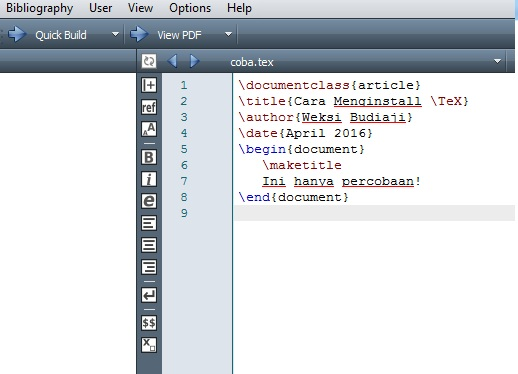
\includegraphics[width=13.54cm,height=9.78cm]{gambar/image1.jpg}}
\caption{Texmaker}
\label{image1.jpg}
\end{figure}

\begin{enumerate}
\setcounter{enumi}{\thenumberedCntC}
\item Setelah menulis file latex seperti diatas, maka save file. Misalkan save dengan nama 'coba'. Kemudian klik tanda panah "\,quick build" atau bisa dengan tekan tombol F6. Untuk melihat hasil pdf nya bisa dengan menekan tombol F7.
\setcounter{numberedCntC}{\theenumi}
\end{enumerate}

\textbf{Macam- macam Editor Latex}

\newcounter{numberedCntE}
\begin{enumerate}
\item \textbf{Emacs dengan AUCTex}
\begin{itemize}
\item OS: Windows, Mac (termasuk fork Aquamacs), Unix
\item Lisensi: Free software (GPL)
\item Bahasa: de, dk, fr, is, it, jp, nl, pl, se, sk didukung oleh AUCTeX
\item Unicode: Ya, sejak Emacs 23
\item RTL/bidirectional support: sejak Emacs 24, melalui bidi-mode
\item \% !TeX directives: Tidak, tetapi Emacs memiliki beberapa realisasi untuk file local variables
\item Syntax highlighting: Ya, bisa diatur lewat customize and Elisp
\item Code completion: Ya, via Emacs Predictive Completion, yang mendukung AUCTeX tanpa konfigurasi lebih lanjut
\item Code folding: Ya
\item Spell checking: Ya
\item SyncTeX: Ya
\item Built-in output viewer: Ya
\item Project management: org-mode, reftex-mode
\end{itemize}
\hspace{0,5in}Emacs adalah salah satu editor tertua, yang mendukung mode penyuntingan LaTeX, ConTeXt, dan Plain TeX, AUCTeX dan paket untuk mengelola kode-kode sumber, RefTeX.

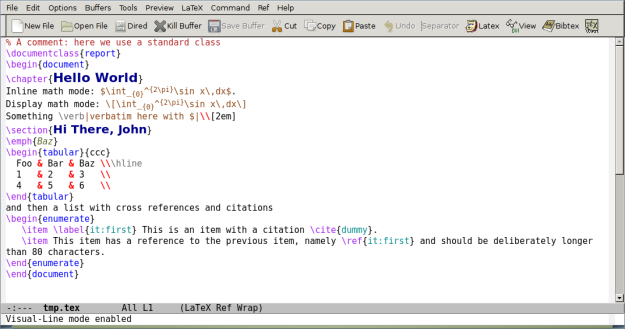
\includegraphics[width=10.95cm,height=7.87cm]{gambar/image2.jpg}
\par \vspace{12pt}

RefTeX membuat seluruh referensi Anda mudah ditemukan layaknya C-c $<$key$>$, baik untuk BibTeX maupun biblatex, dan ia memiliki pintasan (shortcut key) pula untuk bernavigasi di antara bagian-bagian dokumen dengan menggunakan C-c =: secara default.


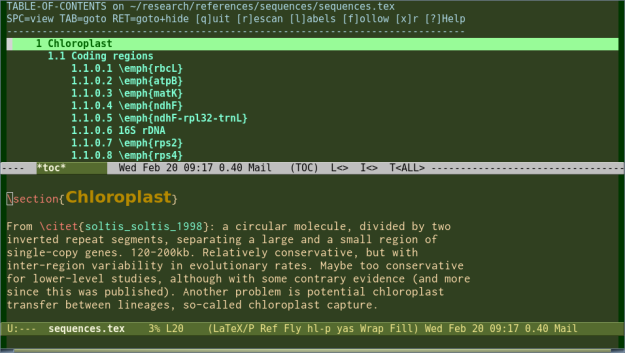
\includegraphics[width=15.64cm,height=8.83cm]{gambar/image3.jpg}

(Tema warna dapat dikonfigurasi sebebas mungkin)

AUCTeX mendukung multi-file parsing, sehingga dokumen-dokumen besar dengan perintah \textit{$\setminus$input} atau \textit{
$\setminus$include} mudah dikompilasikan dengan \textit{C-c C-c} pada berkas yang bersangkutan. Tidak perlu lagi kembali ke master file hanya untuk mengompilasi.
\par \vspace{12pt}
Fitur AUCTeX \textit{preview-latex} adalah pratayang WYSIWYG untuk rumus-rumus. Fitur-fitur terkemuka Emacs:

\begin{itemize}
\item Menggunakan table-insert bersama dengan fungsi
table-generate-source dan table-recognize-* untuk membuat tabel-tabel dengan mudah.
\item Banyak sekali shortcut key tersedia
\item Terdokumentasi dengan baik, baik Emacs itu sendiri melalui manual Emacs dan manual AUCTex Texinfo, maupun melalui banyak buku dalam beberapa bahasa.
\end{itemize}

\item \textbf{Vim dengan LaTeX-suite}
\begin{itemize}
\item OS: Windows, Mac, Linux, BSD, dan lain-lain
\item Lisensi: Open Source Charityware
\item Bahasa: ?
\item Unicode: Ya
\item RTL/bidi support: sebagian
\item \% !TEX directives: Tidak, tetapi memiliki modelines
\item Syntax Highlighting: Ya, bisa dikustomisasi
\item Code Completion: Ya (menggunakan Omni Completion, bisa diperluas dengan plugin SnipMate)
\item Code Folding: Ya
\item Spell Checking: Ya
\item SyncTeX: Ya, lihat pertanyaan ini
\item Built-in Output Viewer: Tidak
\item Project Management: ?
\item Jika Anda benar-benar kelas berat, Anda akan selalu menggunakan Vim. Ada banyak macro yang dibuat untuk Vim untuk membantu menyunting berkas LaTeX.
\end{itemize}
\begin{figure}[ht]

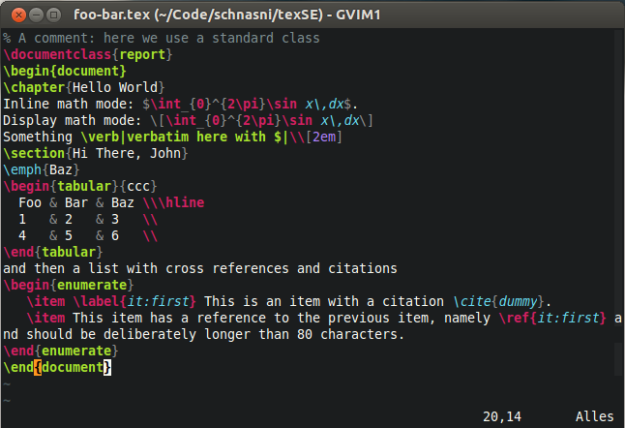
\includegraphics[width=15.57cm,height=10.66cm]{gambar/image4.jpg}
\end{figure}

Anda dapat melakukan word/command completion melalui
\begin{equation}
<C-P> dan <C-N>,
\end{equation}untuk memilih saran sebelumnya atau sesudahnya.

Ada versi Vim dengan menu-menu grafis, yang bernama gVim. Jika ia digunakan dengan Latex-suite, maka banyak perintah TeX ditampilkan di menubar untuk mempercepat penyuntingan.
\par \vspace{12pt}
\textbf{Fitur-Fitur}
\par \vspace{12pt}
Vim juga memiliki fitur code-folding, karena paket vim-late menawarkan code-folding otomatis. Folding juga bisa dilakukan secara manual berdasarkan kunci (misalnya \{\{\{ dan \}\}\}) untuk membuka dan menutup fold otomatis. Contoh folds bisa dilihat pada gambar berikut:

\begin{figure}[ht]

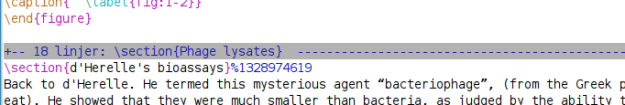
\includegraphics[width=15.12cm,height=2.54cm]{gambar/image5.jpg}
\end{figure}

Fitur Vim masih sangat banyak. Namun di dalam tulisan ini, yang bisa disebutkan adalah:

VIM

Regex

\begin{itemize}
\item Perintah dan pintasan kibor yang powerful
\item Sangat bisa dikustomisasi
\item Smart Indenting
\end{itemize}
LaTeX-Suite

\begin{itemize}
\item Panggil cepat kompiler dengan $\setminus$ll; tayangkan hasil dengan $\setminus$lv
\item Environments dapat diakses dengan tiga huruf dalam insert mode:
\end{itemize}
\hspace{0,2in}EEQ = environment persamaan

EFI = environment gambar (figure)

\begin{itemize}
\item Place-holders ($<$+text+$>$) dapat dilompati dengan Ctrl-J tanpa meninggalkan insert mode
\item Inverse searching: klik ganda penampil PDF dan Anda lompat ke baris kode sumber tex yang bersesuaian.
\end{itemize}

\item \textbf{Texmaker - texmaker}
\begin{itemize}
\item Platforms: Windows XP/Vista/7/8, OS X 10.5+, Linux
\item License: GPL, gratis
\item Languages: cs, de, el, en, es, fa, fr, gl, hu, it, nl, pl, pt, pt (bra), ru, se, sr, zh (cn), zh (tw)
\item Unicode: Ya
\item RTL/bidi: ?
\item \% !TEX directives: Tidak
\item Syntax Highlighting: Ya, bisa dikustomisasi
\item Code Completion: Ya, bisa dikustomisasi
\item Code Folding: Ya
\item Spell Checking: Ya
\item SyncTeX: Ya
\item Built-in Output Viewer: Ya, mendukung PDF
\end{itemize}
\item \textbf{TeXworks - texworks}
\begin{itemize}
\item OS: Windows XP/Vista/7/8, OS X, Linux
\item Lisensi: GPL
\item Bahasa: en, af, ar, ca, cs, de, fa, fo fr, it, ja, nl, ko, pl, pl, ru, sl, tr zh
\item Unicode: Ya
\item RTL/bidi: Ya
\item \% !TEX directives: Ya
\item Syntax Highlighting: Ya, regex-based
\item Code Completion: Ya, bisa dikustomisasi berdasarkan daftar 'known entry'
\item Code Folding: Tidak
\item Spell Checking: Ya, tetapi harus diinstal sendiri
\item SyncTeX: Ya
\item Built-in Output Viewer: Ya, PDF (Poppler-based)
\item Project Management: Tidak
\item Di Windows dan Linux, saya menggunakan TeXworks, yang menyediakan jendela editor kode dan pratayang. Klik pada pratayang dokumen akan langsung menandai kode LaTeX yang bersesuaian.
\end{itemize}

\item \textbf{Kile - kile}
\begin{itemize}
\item OS: Linux, Windows1 (XP, Vista, 7)
\item LIsensi: GNU GPL 2
\item Bahasa:
\begin{verbatim}bg, bs, ca, cs, da, de, el, en\_GB, eo, es, et, fi, fr, ga, gl, hi, hne, hu, it, ja, kk, lt, mai, ms, nb, nds, nl, nn, pl, pt, pt\_BR, ro, ru, sk, sv, tr, ug, uk, zh\_CN, zh\_TW
\end{verbatim}
\item Unicode: Ya
\item RTL/bidi: Ya
\item \% !TEX directives: Tidak2
\item Syntax Highlighting: Ya, bisa dikustomisasi
\item Code Completion: Ya, bisa dikustomisasi
\item Code Folding: Ya
\item Spell Checking: Ya
\item SyncTeX: Ya (namun flag -synctex=1 harus ditambahkan secara manual pada build engine)
\item Built-in Output Viewer: Terbatas3 (pratayang PNG dari sebagian kode - misalnya environment yang dipilih - dikonversikan dari DVI/PS/PDF)
\item Project Management: Ya
\end{itemize}
\begin{figure}[ht]

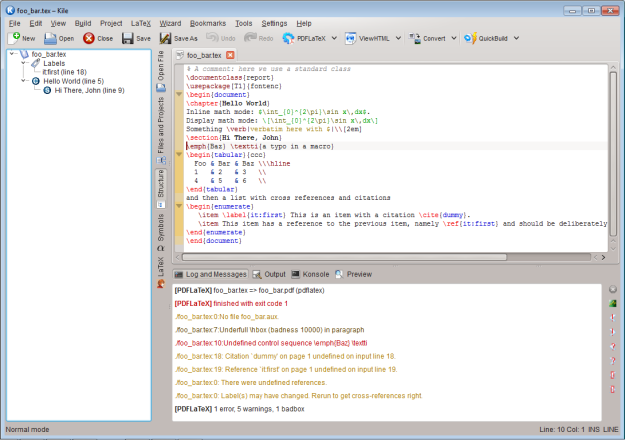
\includegraphics[width=14.76cm,height=10.39cm]{gambar/image6.jpg}
\end{figure}


\item \textbf{TeXstudio - texstudio}

\begin{table}[ht]
	\caption{Instalasi Paket}
	\centering
	\begin{tabular}{cccc}
		\hline
		No&Keterangan&\\
		\hline
		.1&OS: Windows XP/Vista/7, OS X, Linux, FreeBSD&\\
		.2&Lisensi: GPL v2&\\
		.3&Bahasa: cs, de, en, es, fr, hu, ja, pt\_BR, zh\_CN&\\
		.4&Unicode: Ya&\\
		.5&RTL/bidi: ?&\\
		.6&TeX directives: Ya&\\
		.7&Syntax Highlighting: Ya, bisa dikustomisasi&\\
		.8&Code Completion: Ya, bisa dikustomisasi dan auto-customized&\\
		.9&Unicode: Ya&\\
		.10&Code Folding: Ya&\\
		.11&Spell Checking: Ya&\\
		.12&SyncTeX: Ya&\\
		.13&Built-in Output Viewer: Ya, mendukung PDF&\\
		.14&Project Management: Ya&\\
		.15&Saya merekomendasikan TeXstudio sebagai fork yang menarik dari Texmaker yang saya rasa lebih nyaman dan bisa dikustomisasi.&\\
		\hline
	\end{tabular}
\end{table}
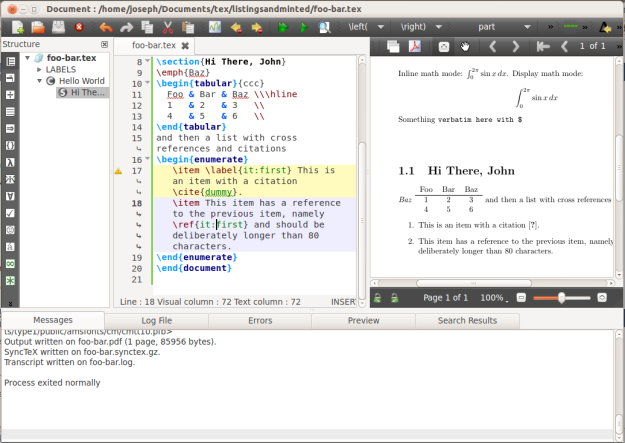
\includegraphics[width=15.23cm,height=10.79cm]{gambar/image7.jpg}

Fitur-fitur lainnya:
\begin{itemize}
\item cross-platform
\item dukungan penulisan (incremental search, folding, navigasi, auto-completion, custom macros)
\item syntax highlighting
\item inline interactive spell-checking
\item mendukung program-program LaTeX utama, termasuk tikz, pstricks, dan lain-lain
\item multi-views: math, structure
\item dukungan SVN
\item bisa berjalan via USB flash disk
\item mendukung synctex
\item termasuk penampil PDF, tetapi masih bisa dikonfigurasi untuk memakai viewer eksternal (juga dengan synctex)
\item developer dan komunitas yang sangat aktif dan responsive
\end{itemize}


\item \textbf{LyX}
\begin{itemize}
\item OS: Windows, Mac, and Linux
\begin{itemize}
\item Lisensi: Open Source
\item Sangat intuitif dan ramah pengguna, dan bisa impor/ekspor ke LaTeX.
\item Terlalu banyak ftur untuk disebutkan, paling bagus: Jika Anda ingin menulis rumus matematika "\,2-dimensional", LyX cocok untuk itu.
\end{itemize}
\end{itemize}
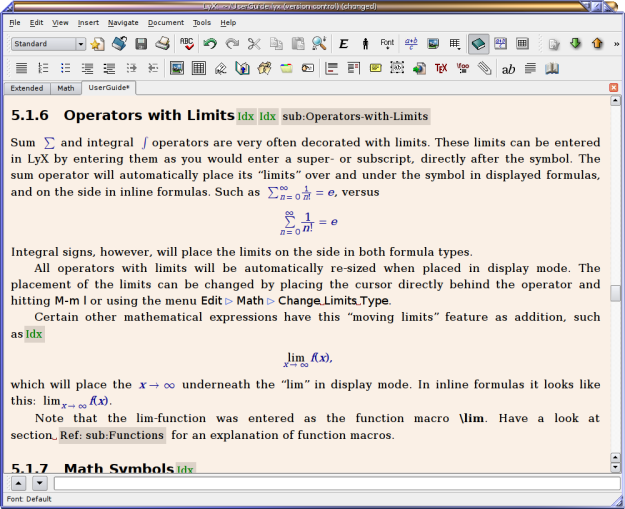
\includegraphics[width=14.10cm,height=11.48cm]{gambar/image8.jpg}

\item \textbf{Sublime Text dengan LaTeX Plugin}
\setcounter{numberedCntE}{\theenumi}
\hspace{0,2in}OS: Windows, Mac, Linux

Ini adalah editor yang sederhana tetapi powerful. Sublime Text mirip Notepad++, tetapi tersedia untuk banyak platform dan sangat mudah diatur untuk LaTeX dengan plugin LaTeXTools atau LaTeXing -keduanya tersedia dari Package Control. Sublime juga mirip TextMate, tetapi dikembangkan lebih aktif dan memiliki komunitas yang besar yang menyediakan plugin-nya. Sublime juga lebih cantik daripada keduanya.
\par \vspace{12pt}

Perhatikan bahwa ini adala software berbayar, dan meminta lisensi selama periode evaluasi (seharga USD 70). Dimungkinkan untuk menjalankan Sublime Text tanpa membeli lisensi, tetapi Anda akan terus diingatkan bahwa Anda menggunakan salinan yang belum diregistrasikan.
\par \vspace{12pt}


Sublime Text memiliki peralatan yang canggih untuk mengetik, yang Anda tidak mau tinggalkan ketika bekerja dengannya:

\begin{itemize}
\item multiple cursors
\item go-to ke mana saja
\item snippets
\item incremental find
\item manajemen proyek
\item build-systems yang banyak
\end{itemize}
dan banyak lagi (lihat Perfect Workflow in Sublime Text 2). Skrinsot di bawah juga menampakkan fiturnya untuk menemukan sitas-sitasi (citations) dari BibTeX.
\par \vspace{12pt}

Sublime Text ini editor yang hampir sempurna, dengan potensi yang hampir tidak terbatas. Daftar fiturnya panjang sekali. Instal Package Manager, dan paket-paket tambahan dari repositori bisa dipasang dalam beberapa detik saja.

\begin{itemize}
\item OS: Windows, Unix
\item Lisensi: Free to try, free to buy
\item \% !TEX directives: Ya
\item Syntax highlighting: Ya
\item Code completion: Ya
\item Code folding: Ya
\item Spell check: Ya, baik built-in maupun dengan plugin
\item SyncTeX: Ya
\item Built-in output viewer: Tidak
\item Project management: Ya
\end{itemize}
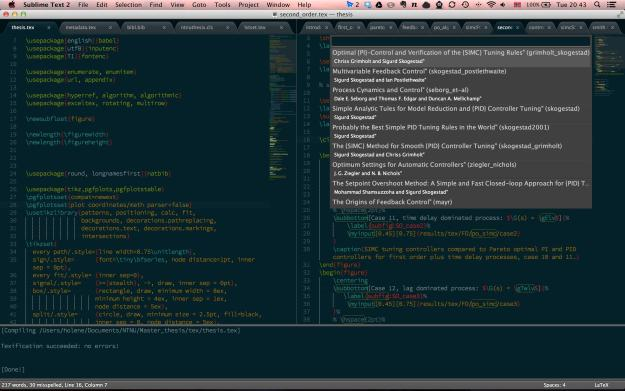
\includegraphics[width=15.67cm,height=9.80cm]{gambar/image9.jpg}

\item \textbf{TeXlipse}
\begin{itemize}
\item OS: Windows, Mac, Linux and others (Java based)
\item Lisensi: Open Source
\end{itemize}
Saya telah berbahagia menggunakan TeXlipse di Eclipse sejak lama, ia memiliki code completion terintegrasi (termasuk entri-entri BibTeX), templat-templat yang mudah dikustomisasi, panel outline, dan secara langsung ia terintegrasi dengan Eclipse itu sendiri yang secara otomatis memiliki shortcuts, version control, dan lain-lain.
\par \vspace{12pt}

Ada plugin penampil PDF untuk Eclipse bernama Pdf4Eclipse dengan dukungan SyncTeX, yang mendukung pencarian maju/mundur di dalam dokumen LaTeX. Karena TeXlipse me-rebuild kode-kode LaTeX secara otomatis (di background) setelah sekali disimpan, maka kode dan pratayang dari dokumen selalu disinkronkan.

\item \textbf{Gummi}
\begin{itemize}
\item OS: Linux (tersedia versi unstable untuk Windows)
\item Lisensi: Open Source
\end{itemize}


Emacs bagus, tetapi yang seringkali saya pakai adalah Gummi. Ia memiliki panel pratayang yang sangat berguna untuk mengetahui kesalahan sintaks dan kesalahan format sesegera mungkin. Plus, ketika Anda menyimpan dokumen LaTeX ia akan menyimpan PDF secara otomatis. Fitur lainnya termasuk peralatan bantuan penulisan matriks, memasukkan gambar, dan
sitasi (citation).
\par \vspace{12pt}

\begin{figure}[ht]

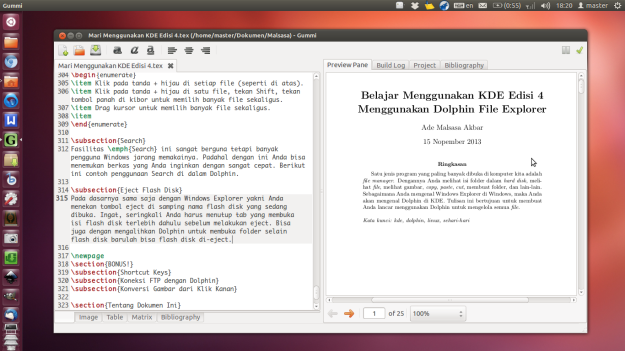
\includegraphics[width=15.45cm,height=8.68cm]{gambar/image10.jpg}
\end{figure}

\item \textbf{LaTeXila}
\begin{itemize}
\item OS: Linux
\item Lisensi: Open source
\item Unicode: Ya
\end{itemize}
\hspace{0,5in}LaTeXila adalah lingkungan LaTeX terintegrasi untuk GNOME. Ia memiliki antarmuka yang bagus dan jelas. Ia tersedia di Ubuntu Software Center. Anda dapat melihat preview dari apa yang Anda tulis kapanpun Anda mau.
\par \vspace{12pt}

LaTeXila memiliki komentar-komentar "\,ajaib" untuk membuat todonotes, yang akan tayang di panel struktur di sebelah kiri. Komentar itu adalah \%TODO dan \%FIXME, yang harus diikuti oleh teks (jika tidak ada teks, maka tidak ada yang tayang di panel).

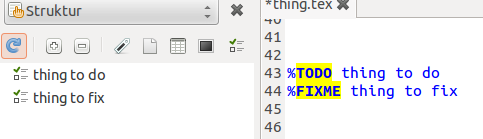
\includegraphics[width=12.78cm,height=3.68cm]{gambar/image11.jpg}


\item \textbf{Geany with GeanyLaTeX}
\begin{itemize}
\item OS: Windows, Mac, Linux dan lain-lain
\item Lisensi: Open Source
\end{itemize}
\end{enumerate}


Editor bagus lainnya adalah Geany. Software ini memiliki plugin untuk LaTeX. Plugin ini di-maintain oleh salah satu developer utama Geany sendiri. Plugin ini memiliki wizard untuk dokumen LaTeX baru, autocompletion, insert environment dengan mudah, dan tentu terdokumentasi dengan baik.



\chapter{Your First Document}
\section {Pengertian Latex}\par



TEX merupakan perangkat lunak pengolah dokumen yang terutama ditujukan menghasilkan dokumen yang berisi simbol-simbol matematik. TEX diciptakan oleh Donald E. Knuth (Mei1977) sebaga ibahasa pembentuk dokumen (document formatting language). LaTeX adalah sistem typesetting yang dapat digunakan untuk membuat artikel, buku, surat, dan publikasi lain berkualitas tinggi. LaTeX berbasiskan pada TeX, bahasa typesetting aras bawah yang didesain oleh Donald E. Knuth. LaTeX tidak bekerja seperti pengolah kata WYSIWYG (what you see is what you get), jenis persiapan dokumen yang sudah banyak dipakai oleh banyak orang. Dengan LaTeX, Anda tidak harus perduli dengan pemformatan dokumen dan tidak perlu mengatur rapi untuk penulisan teks sendiri, hanya tentang penulisan dokumen.


\ref{latex.jpg}:
\begin{figure}[ht]
	\centerline{
\includegraphics[width=10cm,height=7cm]{gambar/latex.jpg}}
	\caption{Latex}
	\label{latex.jpg}
\end{figure}

Perangkat lunak TEX memiliki kemampuan yang baik untuk mengolah dokumen-dokumen yang berkualitas tinggi. Kelemahannya, perintah perintahnya sulit digunakan untuk menuliskan dokumen terstruktur yang terdiri dari unsur-unsur bab, sub-bab, paragraph, table dan gambar bernomor, dsb.\par 
\vspace{12pt}

Versi LATEX yang sudah baku ini memiliki beberapa kekuatan, diantaranya adalah:

\begin{itemize}
\item Standard yang sangat baik untuk menyiapkan tulisan teks,formula 
teknis, dan tabel-tabel
\item Kemudahan penggunaan oleh penulis naskah.
\item Portabilitas dokumen pada berbagai platform
\item Adaptabilitas terhadap banyak bahasa (multilingual support)
\item Ketersediaan secara meluas dan bebas
\item Penulisan menjadi baik dan terstruktur rapi.
\item jenis Matematis dapat dituliskan dengan mudah.
\end{itemize}
\hspace{0,5in}Sebuah dokumen LATEX memiliki struktur yang dicirikan dengan blok yang diapit oleh pasangan perintah $\setminus$begin dan $\setminus$end. 
Untuk menyatakan jenis dokumen yang akan diolah, setiap dokumen harus dimulai dengan perintah:\par \vspace{12pt} $\setminus$documentclass\{\ldots \}\par \vspace{12pt}


Membuat dokumen dengan latex sangat sederhana. Anda bisa memulai membuat dokumen latex dengan mengetikan kode latex lalu ditambah dengan konten yang sederhana yaitu teks. Latex menggunakan kode-kode perintah yang terkontrol yang nantinya akan menentukan seperti apa hasil akhir dari dokumen yang anda buat. Setelah anda mengetikan kode-kode perintah latex, maka compiler dari editor latex dapat mengkompilasinya menjadi file .pdf. \par \vspace{12pt} 


\begin{table}[ht]
	\caption{Instalasi Paket}
	\centering
	\begin{tabular}{cccc}
		\hline
		No&Kelebihan&Kekurangan&\\
		\hline
		1.&Cocok untuk programmer&tidak user friendly seperti ms word&\\
		2.&Filenya relatif kecil&Harus hafal command&\\
		3.&Hasil tampilan dokumen profesional& Cocok untuk data skala besar&\\
		\hline
	\end{tabular}
\end{table}

\subsection {Kelas Dokumen}\par
\vspace{12pt}
Jenis dokumen yang akan diolah ditentukan oleh perintah pertama dalam bentuk: \par \vspace{12pt} $\setminus$documentclass$[$option$]$\{class\}\par \vspace{12pt}

Dalam perintah diatas,"\,class"dapat diganti oleh article, report, book, atau slides untuk menuliskan artikel, laporan, buku, atau transparansi untuk seminar. Sedangkan pada bagian"\,option" dapat dituliskan satu 
atau beberapa pilihan berikut : 10pt, 11pt, 12pt untuk menyatakan ukuran font utama yang digunakan didalam dokumen A4 paper, letterpaper menyatakan ukuran kertas yang digunakan titlepage, notitlepage untuk menyatakan apakah halaman judul akan dibuat terpisah dari badan dokumen atau tidak twocolumn untuk menampilkan dokumen dalam bentuk dua kolom twoside, oneside untuk menyatakan apakah dokumen akan dicetak pada satu 
sisi atau dua sisi dari kertas. contoh dasar menggunakan kode perintah dalam latex yaitu:\par \vspace{12pt}

$\setminus$documentclass\{article\}\par \vspace{12pt}

$\setminus$begin\{document\}\par \vspace{12pt}

Hello World!\par \vspace{12pt}

$\setminus$end\{document\}\par \vspace{12pt}

Kode diatas jika di compile maka akan muncul tulisan "\,Hello World!" 
dalam bentuk file .pdf.\par \vspace{12pt}

\textbf{Perintah-Perintah LATEX}

\newcounter{numberedCntB}
\begin{enumerate}
\item \textbf{Spasi dalam Latex}
\setcounter{numberedCntB}{\theenumi}
\end{enumerate}
Ada perintah khusus untuk membuat spasi dengan panjang tertentu baik secara horizontal maupun vertikal, yaitu :

\begin{itemize}
\item Jika ingin membuat jarak dengan panjang tertentu antara 2 baris, dapat menggunakan tanda ' $\setminus$$\setminus$ ' di akhir baris. Dan juga dapat menentukan sendiri panjang baris kosong dengan menggunakan perintah seperti contoh berikut ini :
\end{itemize}
\hspace{0,2in}baris 1 $\setminus$$\setminus$

$\setminus$vspace\{2cm\}

baris 2 $\setminus$$\setminus$

\par \vspace{12pt}

Dengan perintah ini, Latex akan mengosongkan baris-baris sepanjang 2 cm. Tanpa menggunakan perintah ini untuk membuat spasi dalam teks dokumen, Latex akan tetap menganggapnya 1 spasi.

\begin{itemize}
\item Jika ingin membuat spasi sejauh beberapa centimeter antara 2 kata dibutuhkan perintah sebagai berikut :
\end{itemize}
\hspace{0,5in}kata 1 $\setminus$hspace\{2cm\} kata 2\par \vspace{12pt}

Dengan perintah ini, Latex akan membuat spasi sejauh 2 centimeter.

Jadi, secara umum aturan yang dapat dipakai adalah akhiri paragraf dengan tanda ' $\setminus$$\setminus$ ' dan berikan 1 baris kosong antara tiap-tiap paragraf dan 1 spasi kosong antara masing-masing kata.

\begin{enumerate}
\setcounter{enumi}{\thenumberedCntB}
\item \textbf{Alignment dalam Latex}
\setcounter{numberedCntB}{\theenumi}
\end{enumerate}
\hspace{0,5in}Alignment/perataan baris pada Latex merupakan fitur untuk mengatur perataan teks yang terbagi menjadi rata kiri, rata kanan, atau rata tengah. Semua dokumen dalam Latex secara default diatur memiliki perataan justified (rata kanan kiri).

\begin{itemize}
\item Jika ingin mengatur dokumen rata kiri digunakan perintah sebagai berikut :
\end{itemize}
\hspace{0,5in}$\setminus$begin\{raggedright\}

\hspace{0,5in}isi dokumen yang diatur dengan rata kiri

\hspace{0,5in}$\setminus$end\{raggedright\}

\begin{itemize}
\item Jika ingin mengatur dokumen rata kanan digunakan perintah sebagai berikut :
\end{itemize}
\hspace{0,5in}$\setminus$begin\{raggedleft\}

\hspace{0,5in}isi dokumen yang diatur dengan rata kanan

\hspace{0,5in}$\setminus$end\{raggedleft\}

\begin{itemize}
\item Jika ingin mengatur dokumen rata tengah digunakan perintah sebagai berikut :
\end{itemize}
\hspace{0,5in}$\setminus$begin\{center\}

\hspace{0,5in}isi dokumen yang diatur dengan rata tengah

\hspace{0,5in}$\setminus$end\{center\}

\begin{enumerate}
\setcounter{enumi}{\thenumberedCntB}
\item \textbf{Bahasa dalam Latex}
\setcounter{numberedCntB}{\theenumi}
\end{enumerate}
\hspace{0,5in}Latex dapat menggunakan tulisan mengikuti aturan ejaan yang dimiliki bahasa tertentu. Kemampuan ini diatur oleh babel package. Mengubah peraturan bahasa dengan menggunakan babel akan secara otomatis mengubah nama-nama dari unit struktur dokumen (misalnya Abstract, Chapter, Index) 
menjadi terjemahannya.\par \vspace{12pt}

Perintah yang mengatur latex untuk menggunakan babel bahasa Indonesia seperti berikut :

$\setminus$dokumenclass \{a4paper, 12pt\}\{report\}\par \vspace{12pt}

$\setminus$usepage$[$bahasa$]$\{babel\}\par \vspace{12pt}

$\setminus$begin\{document\}\par \vspace{12pt}

. . . . . . . . . . . . . . . . . . . . .

. . . . . . . . . . . . . . . . . . . . .
\par \vspace{12pt}
$\setminus$end\{document\}

\begin{enumerate}
\setcounter{enumi}{\thenumberedCntB}
\item \textbf{Keterangan dalam Latex}
\setcounter{numberedCntB}{\theenumi}
\end{enumerate}
\hspace{0,5in}Jika Anda ingin menambahkan keterangan pada file yang tidak ingin tercetak, caranya adalah dengan menambahkan tanda \% diawal setiap baris keterangan. Contoh :\par \vspace{12pt}

$\setminus$dokumenclass \{a4paper, 12pt\}\{report\}\par \vspace{12pt}

$\setminus$usepage$[$bahasa$]$\{babel\}\par \vspace{12pt}

$\setminus$begin\{document\}\par \vspace{12pt}

ini baris keterangan, baris ini tidak akan tercetak dalam file 
keluaran

. . . . . . . . . . . . . . . . . . . . .\par \vspace{12pt}

$\setminus$end\{document\}

\begin{enumerate}
\setcounter{enumi}{\thenumberedCntB}
\item \textbf{Font dalam Latex}
\setcounter{numberedCntB}{\theenumi}
\end{enumerate}
Ada 3 jenis fonts dalam Latex :

\begin{itemize}
\item Roman. Cara menggunakannya seperti dibawah ini :
\end{itemize}
\hspace{0,5in}\{$\setminus$rmfamily teks yang ingin diformat \}

\begin{itemize}
\item Sans serif. Cara menggunakannya seperti dibawah ini :
\end{itemize}
\hspace{0,5in}\{$\setminus$sffamily teks yang ingin diformat \}

\begin{itemize}
\item Typewriter. Cara menggunakannya seperti dibawah ini :
\end{itemize}
\hspace{0,5in}\{$\setminus$ttfamily teks yang ingin diformat \}\par \vspace{12pt}



Ada 4 bentuk font dalam Latex :

\begin{itemize}
\item Italic. Cara mengaturnya sebagai berikut :
\end{itemize}
\hspace{0,5in}\{$\setminus$itshape teks yang ingin diformat \}

\begin{itemize}
\item Slanted. Cara mengaturnya sebagai berikut :
\end{itemize}
\hspace{0,5in}\{$\setminus$slshape teks yang ingin diformat \}

\begin{itemize}
\item Vertical. Cara mengaturnya sebagai berikut :
\end{itemize}
\hspace{0,5in}\{$\setminus$upshape teks yang ingin diformat \}

\begin{itemize}
\item SMALL CAPS. Cara mengaturnya sebagai berikut :
\end{itemize}
\hspace{0,5in}\{$\setminus$scshape teks yang ingin diformat \}
\par \vspace{12pt}


Ukuran Font

Ada beberapa macam ukuran font dalam Latex. Untuk menggunakan 
ukuran-ukuran tersebut, cara yang dapat digunakan adalah sebagai berikut :

\begin{itemize}
\item Tiny
\end{itemize}
\hspace{0,5in}\{$\setminus$tiny teks yang ingin diformat \}

\begin{itemize}
\item Scriptsize
\end{itemize}
\hspace{0,5in}\{$\setminus$scriptsize teks yang ingin diformat \}

\begin{itemize}
\item Footnotesize
\end{itemize}
\hspace{0,5in}\{$\setminus$footnotesize teks yang ingin diformat \}

\begin{itemize}
\item Small
\end{itemize}
\hspace{0,5in}\{$\setminus$small teks yang ingin diformat \}

\begin{itemize}
\item Normal
\end{itemize}
\hspace{0,5in}\{$\setminus$normalsize teks yang ingin diformat \}

\begin{itemize}
\item Large
\end{itemize}
\hspace{0,5in}\{$\setminus$large teks yang ingin diformat \}

\begin{itemize}
\item Larger
\end{itemize}
\hspace{0,5in}\{$\setminus$Large teks yang ingin diformat \}

\begin{itemize}
\item Largest
\end{itemize}
\hspace{0,5in}\{$\setminus$LARGE teks yang ingin diformat \}

\begin{itemize}
\item Huge
\end{itemize}
\hspace{0,5in}\{$\setminus$huge teks yang ingin diformat \}

\begin{itemize}
\item Huger
\end{itemize}
\hspace{0,5in}\{$\setminus$Huge teks yang ingin diformat \}

\begin{enumerate}
\setcounter{enumi}{\thenumberedCntB}
\item \textbf{Struktur Dasar Sebuah Dokumen Latex}
\setcounter{numberedCntB}{\theenumi}
\end{enumerate}
\subsection {Document Class}\par \vspace{12pt}

Document class dalam Latex berguna untuk menentukan layout halaman, jenis heading, dan bebagai perintah juga environment yang digunakan untuk mengatur style dokumen. Cara mendeklarasikannya adalah sebagai berikut :\par \vspace{12pt}

$\setminus$dokumentclass \{class\}\par \vspace{12pt}

Ada beberapa jenis document class yang bisa dipakai dalam sebuah dokumen Latex, yaitu :

\begin{itemize}
\item report : dapat digunakan untuk membuat laporan (report) baik dalam bidang bisnis, teknik, hukum, akademis, atau ilmu pengetahuan.
\item article : dapat digunakan untuk membuat paper, artikel sebuah jurnal atau majalah, review, paper untuk konferensi, atau catatan riset.
\item book : dapat digunakan untuk mebuat buku dan thesis.
\item letter : dapat digunakan untuk membuat surat.
\end{itemize}
\hspace{0,5in}Biasanya kelas 'article' adalah yang paling sering digunakan untuk sembarang jenis dokumen.\par \vspace{12pt}



\textbf{Document Class Option}\par \vspace{12pt}

Merupakan pilihan yang tersedia pada kelas dokumen yang bisa ditentukan sendiri isinya. Opsi pada suatu kelas dokumen dituliskan sebagai berikut :\par \vspace{12pt}

$\setminus$dokumentclass $[$option1, option2$]$\{class\}
\par \vspace{12pt}


Default opsi yang digunakan oleh Latex sebagai berikut :

\begin{itemize}
\item Ukuran kertas yang digunakan adalah A4.
\item Ukuran font yang digunakan adalah 10pt untuk semua kelas dokumen.
\item Layout halaman yang digunakan adalah two-sided printing khusus untuk kelas book dan report; dan one-sided printing khusus untuk kelas article dan letter.
\item Halaman judul yang terpisah dibagian awal dokumen khusus untuk kelas book dan report.
\item  Ukuran font dapat disesuaikan dengan kebutuhan masing-masing.
\end{itemize}
Opsi diatas dapat dimodifikasikan sebagai berikut :

\begin{itemize}
\item Ukuran kertas. Dapat ditentukan sendiri ukuran kertasnya. Cara 
penulisannya :
\end{itemize}
\hspace{0,5in}$\setminus$documentclass $[$ a3paper $]$ \{class\}

\hspace{0,5in}atau

\hspace{0,5in}$\setminus$documentclass $[$ letterpaper $]$ \{class\}

\begin{itemize}
\item Ukuran font. Dapat memilih ukuran 10pt, 11pt, atau 12pt. Cara penulisannya :
\end{itemize}
\hspace{0,5in}$\setminus$documentclass $[$ a4paper, 11pt $]$ \{class\}\par \vspace{12pt}

Setelah menentukan ukuran font yang dipakai, semua font yang ada dalam dokumen akan diatur sesuai dengan ukuran yang ditentukan.\par \vspace{12pt}

Layout halaman. Dapat ditentukan dengan pilihan berikut :\par \vspace{12pt}

\begin{itemize}
\item oneside : jika ingin layout one-sided printing saat menggunakan kelas book dan report.
\item twoside : jika ingin layout two-sided printing saat menggunakan kelas article.
\item titlepage : jika ingin kelas article untuk memiliki halaman judul yang terpisah dibagian awal dokumen.
\item draft : berguna untuk mengatur Latex supaya menandai 
masalah-masalah yang timbul seperti masalah pemenggalan kata ( 
pemenggalan kata tidak tepat ) atau masalah perataan tulisan ( ada baris tertentu melebihi batas kanan dokumen ).
\end{itemize}




\textbf{Paket-Paket dalam Latex}\par \vspace{12pt}

Merupakan fungsi-fungsi yang dipakai untuk menambah kemampuan Latex melakukan pengaturan dokumen. Cara menggunakan paket yang sudah tersedia/terintegrasi di dalam Latex sebagai berikut :
\par \vspace{12pt}
$\setminus$documentclass \{class\}\par \vspace{12pt}

$\setminus$usepackage $[$ option $]$ \{nama paket\}\par \vspace{12pt}

$\setminus$begin\{document\}\par \vspace{12pt}

. . . . . . . . . . . . . . . . . .

. . . . . . . . . . . . . . . . . .
\par \vspace{12pt}
$\setminus$end\{document\}\par \vspace{12pt}

Beberapa paket yang tersedia dalam Latex sebagai berikut :

\begin{itemize}
\item graphicx : dapat menghasilkan gambar grafis dan juga membuat Latex mampu menampilkan gambar yang kita sertakan dalam dokumen.
\item hyperref : dapat menghasilkan dokumen yang memiliki dynamic link ke alamat tertentu.
\item babel : dapat mengenali format bahasa yang digunakan.
\item color : dapat menghasilkan teks dokumen yang memiliki warna sesuai warna yang ditentukan.
\item makeidx : dapat menghasilkan indeks dari dokumen yang dibuat.
\item 
\end{itemize}
\textbf{Document Environment}\par \vspace{12pt}

Merupakan bagian dalam sebuah dokumen Latex dimana isi sebenarnya dari dokumen itu sendiri ditempatkan.
\par \vspace{12pt}
$\setminus$documentclass \{class\}\par \vspace{12pt}

$\setminus$begin\{document\}\par \vspace{12pt}

. . . . . . . . . . . . . . . . . .

. . . . . . . . . . . . . . . . . .\par \vspace{12pt}

$\setminus$end\{document\}\par \vspace{12pt}

Struktur $\setminus$begin . . . . $\setminus$end inilah yang disebut dengan environment. Environment membatasi bagian teks yang akan diatur dengan aturan tertentu.\par \vspace{12pt}

\subsection {Penulisan Judul}\par \vspace{12pt}

Judul dalam sebuah dokumen Latex diletakan pada awal document 
environment. Cara penulisannya adalah sebagai berikut :\par \vspace{12pt}

$\setminus$documentclass $[$ a4paper, 12pt $]$ \{report\}\par \vspace{12pt}

$\setminus$begin\{document\}\par \vspace{12pt}

$\setminus$title\{Judul Dokumen\}\par \vspace{12pt}

$\setminus$autor\{Nama Penulis\}\par \vspace{12pt}

$\setminus$date\{Tanggal Pembuatan\}\par \vspace{12pt}

$\setminus$maketitle\par \vspace{12pt}

. . . . . . . . . . . . . . . . . .

. . . . . . . . . . . . . . . . . .\par \vspace{12pt}

$\setminus$end\{document\}\par \vspace{12pt}



\subsection {Abstrak}\par \vspace{12pt}

Pada dokumen kelas article dan report umumnya memiliki 
abstrak/ringkasan. Latex memiliki cara khusus untuk menuliskan abstrak. Penulisannya adalah sebagai berikut :\par \vspace{12pt}

$\setminus$documentclass $[$ a4paper, 12pt $]$ \{report\}\par \vspace{12pt}

$\setminus$begin\{document\}\par \vspace{12pt}

$\setminus$title\{Judul Dokumen\}\par \vspace{12pt}

$\setminus$autor\{Nama Penulis\}\par \vspace{12pt}

$\setminus$date\{Tanggal Pembuatan\}\par \vspace{12pt}

$\setminus$maketitle\par \vspace{12pt}

$\setminus$begin\{abstract\}\par \vspace{12pt}

isi abstrak\par \vspace{12pt}

$\setminus$end\{abstract\}\par \vspace{12pt}

. . . . . . . . . . . . . . . . . .\par \vspace{12pt}

$\setminus$end\{document\}\par \vspace{12pt}

Jika ingin mengubah judul abstrak digunakan perintah sebelum 
$\setminus$begin\{abstract\} :

$\setminus$renewcommand \{$\setminus$abstractname\}\{Ringkasan Laporan\}\par \vspace{12pt}

Contoh diatas dapat mengganti judul abstrak menjadi "\, Ringkasan Laporan "\,.\par \vspace{12pt}

\subsection {Daftar Berurut}\par \vspace{12pt}

Ada 3 cara penulisan daftar berurut, yaitu :

Daftar dengan penomoran dengan menggunakan simbol (Bulleted List), contoh :

Mobil\par \vspace{12pt}

Montor\par \vspace{12pt}

Sepeda\par \vspace{12pt}

Bus\par \vspace{12pt}

Cara penulisannya dalam Latex adalah sebagai berikut :\par \vspace{12pt}

$\setminus$begin\{itemize\}\par \vspace{12pt}

$\setminus$item . . . .\par \vspace{12pt}

$\setminus$item . . . .\par \vspace{12pt}

$\setminus$item . . . .\par \vspace{12pt}

$\setminus$item . . . .\par \vspace{12pt}

. . . . .

. . . . .\par \vspace{12pt}

$\setminus$end\{itemize\}\par \vspace{12pt}



\subsection {Daftar Isi}\par \vspace{12pt}

Untuk menampilkan daftar isi dapat menggunakan perintah :\par \vspace{12pt}

$\setminus$tableofcontents\par \vspace{12pt}

Perintah ini diletakan pada bagian dimana daftar isi tersebut 
ditempatkan. Biasanya daftar isi ditempatkan setelah abstrak/kata pengantar.

Untuk menampilkan daftar gambar dapat menggunakan perintah :\par \vspace{12pt}

$\setminus$listoffigures\par \vspace{12pt}

Untuk menampilkan daftar tabel dapat menggunakan perintah :\par \vspace{12pt}

$\setminus$listoftables
\par \vspace{12pt}
Latex menghasilkan file berekstensi *.toc untuk daftar isi, daftar gambar, dan daftar tabel. Jika daftar isi, daftar gambar dan daftar tabel tidak menampilkan keseluruhan struktur dokumen dengan benar, dapat diatur seendiri isinya dengan perintah berikut ini :\par \vspace{12pt}

$\setminus$addcontensline\{toc\}\{struktur\}\{teks yang ingin 
ditampilkan pada daftar isi\}\par \vspace{12pt}

Struktur dapat diisi dengan chapter, section, subsection, dll, 
tergantung dengan bagian dokumen yang ingin dimasukkan dalam daftar isi. Dengan perintah diatas, Latex akan menghasilkan baris baru dalam daftar isi dan akan secara otomatis menentukan nomor halaman bagian tersebut.\par \vspace{12pt}

\textbf{Gambar}\par \vspace{12pt}

Agar Latex mendapatkan gambar dalam dokumen, maka perlu mendeklarasikan penggunaan paket graphicx pada bagian preambel. Cara mendeklarasikannya adalah :\par \vspace{12pt}

$\setminus$usepackage\{graphicx\}\par \vspace{12pt}

Untuk menempatkan sebuah gambar dalam dokumen Latex, dapat dengan cara berikut :

$\setminus$begin\{figure\}$[$htbp$]$
\par \vspace{12pt}
$\setminus$caption\{Nama Gambar\}
\par \vspace{12pt}
$\setminus$begin\{center\}
\par \vspace{12pt}

$\setminus$includegraphicx$[$width=2cm,height=3cm$\setminus$columnwidth$]$\{nama file gambar\}
\par \vspace{12pt}
$\setminus$end\{center\}
\par \vspace{12pt}
$\setminus$end\{figure\}
\par \vspace{12pt}


Ada beberapa hal yang perlu diketahui dalam format perintah diatas :

\begin{itemize}
\item Panjang dan lebar dari gambar yang akan ditampilkan dapat ditentukan sesuai keinginan. Isi dari width dapat diisi dengan lebar gambar dan isi dari height dapat diisi dengan tinggi gambar tersebut; 
keduanya harus dilengkapi dengan dimensi dari ukuran panjang yang digunakan.
\item File gambar yang ingin dimasukkan dalam dokumen, harus diletakkan pada direktori yang sama dengan direktori file dokumen (*.tex).
\end{itemize}

\begin{itemize}
\item Pengaturan posisi gambar dapat diatur sesuai dengan 2 hal :
\begin{itemize}
\item Perataan terhadap tepi dokumen : dengan mengubah 
$\backslash$begin\{center\} dan juga $\backslash$end\{center\} dapat menentukan posisi gambar terhadap tepi dokumen.
\item Huruf-huruf pada $\backslash$begin\{figure\}$[$htbp$]$ berfungsi sebagai pengatur posisi gambar pada suatu halaman.
\begin{itemize}
\item h : tabel diletakan persis ditempat perintah tersebut dituliskan pada dokumen.
\item t : tabel diletakan dibagian atas halaman.
\item b : tabel diletakan dibagian bawah halaman.
\item p : tabel diletakan pada sebuah halaman khusus yang hanya memuat tabel itu saja.
\end{itemize}
\end{itemize}
\end{itemize}
Saat menggunakan pengaturan h, Latex akan otomatis menempatkan gambar dihalaman baru jika tidak ada cukup ruang untuk gambar tersebut ditempat perintah gambar dituliskan.\par \vspace{12pt}

Format gambar standar Latex adalah *.eps. Tetapi gambar dengan format *.jpg juga bisa digunakan.\par \vspace{12pt}

\subsection {Daftar Pustaka}\par \vspace{12pt}

Untuk menampilkan daftar pustaka pada akhir sebuah dokumen Latex menggunakan format perintah sebagai berikut :\par \vspace{12pt}

$\setminus$begin \{thebibliography\}\{99\}
\par \vspace{12pt}
$\setminus$bibitem \{label untuk referensi\}\{keterangan pustaka yang digunakan\}
\par \vspace{12pt}
. . . . . . . . . . . . .

. . . . . . . . . . . . .
\par \vspace{12pt}
$\setminus$end \{thebibliography\}
\par \vspace{12pt}


Beberapa hal yang perlu diketahui dalam perintah diatas :

\begin{itemize}
\item Angka 99 memberitahukan Latex bahwa penomoran maksimal Daftar pustaka adalah 99.
\item Label untuk referensi diisikan keyword yang akan digunakan saat membuat rujukan ke pustaka yang bersangkutan.
\item Keterangan pustaka diisi informasi mengenai : penulis, judul pustaka, edisi, penerbit, kota penerbit, dan tahun penerbit.
\end{itemize}


\textbf{Notasi Matematika dalam Latex}\par \vspace{12pt}

\textbf{Penulisan Notasi Matematika dalam Paragraf}\par \vspace{12pt}

Untuk menyisipkan notasi matematika dalam suatu kalimat/paragraf menggunakan perintah berikut ini :
\par \vspace{12pt}
$\setminus$begin\{math\} . . . . . $\setminus$end\{math\} atau
\par \vspace{12pt}
\$ . . . . . . . . . \$
\par \vspace{12pt}


Titik-titik tersebut diisi dengan notasi matematika yang disisipkan.\par \vspace{12pt}

\textbf{Paragraf Khusus Matematika}
\par \vspace{12pt}
Untuk menuliskan notasi matematika yang panjang, dapat memillih untuk menuliskannya dalam paragraf baru. Perintahnya :
\par \vspace{12pt}
$\setminus$begin\{displaymath\}
\par \vspace{12pt}
. . . . . . . .
\par \vspace{12pt}
$\setminus$end\{displaymath\}
\par \vspace{12pt}


Titik-titik tersebut diisi dengan notasi matematika yang disisipkan.
\par \vspace{12pt}
\textbf{Font dalam Matematika}
\par \vspace{12pt}
Ada beberapa perintah yang digunakan untuk mengubah jenis font yang dipakai dalam notasi matematika, seperti berikut ini :
\par \vspace{12pt}
Perintah \$$\setminus$mathrm\{x y z\}\$ 
akan menghasilkan :

xyz
\par \vspace{12pt}
Perintah \$$\setminus$mathsf\{x y z\}\$ 
akan menghasilkan :

xyz
\par \vspace{12pt}
Perintah \$$\setminus$mathtt\{x y z\}\$ 
akan menghasilkan :

xyz
\par \vspace{12pt}
Perintah \$$\setminus$mathit\{x y z\}\$ 
akan menghasilkan :

xyz\par \vspace{12pt}



Perintah \$$\setminus$mathbf\{x y z\}\$ 
akan menghasilkan :

xyz
\par \vspace{12pt}
Perintah \$$\setminus$mathcal\{x y z\}\$ 
akan menghasilkan :

xyz
\par \vspace{12pt}
Untuk menuliskan font matematika dalam bentuk superscripts dan 
subscripts digunakan aturan beikut ini :\par \vspace{12pt}

Superscripts, cara penulisannya dengan perintah $\setminus$sp\{ . . . 
\} atau dengan tanda \^{}.
\par \vspace{12pt}
Subscripts, cara penulisannya dengan perintah $\setminus$sb\{ . . . \} 
atau dengan tanda \_.
\par \vspace{12pt}
Contoh :
\par \vspace{12pt}
$\setminus$begin\{displaymath\}
\par \vspace{12pt}

y=x$\setminus$sb\{1\}$\setminus$sp\{2\}+x$\setminus$sb\{2\}$\setminus$sp\{2\}
\par \vspace{12pt}
$\setminus$end\{displaymath\}
\par \vspace{12pt}


\subsection {Penulisan Pecahan}
\par \vspace{12pt}
Untuk menghasilkan notasi pecahan dengan format perintah sebagai berikut:\par \vspace{12pt}

$\setminus$frac\{numerator\}\{denominator\}
\par \vspace{12pt}
Contoh :
\begin{equation}
frac\{a+2b\}\{a-1\}
\end{equation}


\textbf{Penulisan Array dan Matriks}
\par \vspace{12pt}
Sebuah array/matriks dituliskan dalam environment tabular sama seperti cara pembuatan tabel. Perintahnya sebagai berikut :
\par \vspace{12pt}
$\setminus$begin\{displaymath\}
\par \vspace{12pt}
$\setminus$left (
\par \vspace{12pt}
$\setminus$begin\{array\}\{rrr\}
\par \vspace{12pt}
0 \& 45 \& 23 $\setminus$$\setminus$
\par \vspace{12pt}
34 \& -93 \& 68 $\setminus$end\{array\}
\par \vspace{12pt}
$\setminus$right )
\par \vspace{12pt}
$\setminus$end\{displaymath\}
\par \vspace{12pt}


Beberapa hal yang perlu diketahui dari format perintah itu :

\begin{itemize}
\item Sama seperti penulisan tabel, huruf r dibagian belakang 
$\setminus$begin\{array\}\{rrr\} fungsinya menentukan posisi dari masing-masing komponen matriks tersebut. Dalam hal ini komponen masing-masing matriks dibuat menjadi rata kanan.
\item Tanda kurung yang digunakan adalah tanda kurung kurawal. Bagian kurung buka dan tutup didefinisikan masing-masing.
\end{itemize}


\textbf{Penulisan Vektor}\par \vspace{12pt}

Penulisan vektor dalam Latex menggunakan perintah berikut ini :
\begin{verbatim}
\par \vspace{12pt}
$\setminus$begin\{displaymath\}
\par \vspace{12pt}
$\setminus$vac\{variabel\}
\par \vspace{12pt}
$\setminus$end\{displaymath\}
\par \vspace{12pt}
Contoh :
\par \vspace{12pt}
$\setminus$begin\{displaymath\}
\par \vspace{12pt}
$\setminus$vac\{a\}
\par \vspace{12pt}
$\setminus$end\{displaymath\}
\par \vspace{12pt}
\end{verbatim}



\chapter{Structuring Your Document (Section and Paragraph)}
\section{Structuring Your Document}

\hspace{0.50in} Membuat dokumen yang sangat mendasar telah kita pelajari dalam materi sebelumnya, namun saat menulis makalah Anda perlu menyusun konten ke dalam unit logika. Untuk mencapai hal ini, LaTeX menawarkan perintah untuk menghasilkan judul bagian dan mencatatnya secara otomatis. Perintah untuk membuat judul bagian sangat mudah: \par
{\fontsize{10pt}{10pt}\selectfont  $  \setminus  $section $  \{  $ $  \}  $}
 \par
{\fontsize{10pt}{10pt}\selectfont  $  \setminus  $subsection $  \{  $ $  \}  $}
 \par
{\fontsize{10pt}{10pt}\selectfont  $  \setminus  $subsubsection $  \{  $ $  \}  $}
 \par
{\fontsize{10pt}{10pt}\selectfont  $  \setminus  $paragraph $  \{  $ $  \}  $}
 \par
{\fontsize{10pt}{10pt}\selectfont  $  \setminus  $subparagraph $  \{  $ $  \}  $}
 \par

Hasil \ref{dokumen} Dokumen:
\begin{figure}[ht]
	\centerline{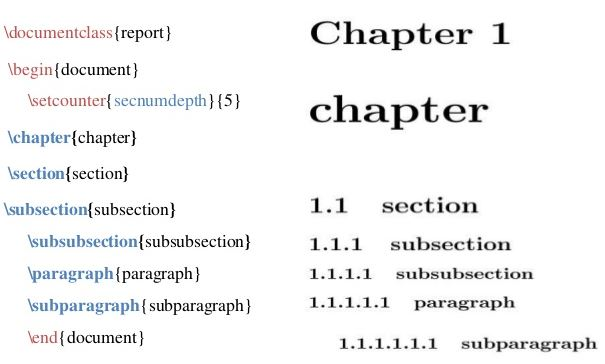
\includegraphics[width=0.50\textwidth]{gambar/dokumen}}
	\caption{dokumen}
	\label{dokumen}
\end{figure}

\vspace{50pt}
\hspace{0.50in} Sedangkan dokumen kelas report dan book selain memiliki perintah-perintah di atas memiliki juga perintah :
 \par
{\fontsize{10pt}{10pt}\selectfont  $  \setminus  $part $  \{  $... $  \}  $}
 \par
\vspace{9pt}

{\fontsize{10pt}{10pt}\selectfont  $  \setminus  $chapter $  \{  $... $  \}  $}
 \par
\vspace{9pt}
{\fontsize{10pt}{10pt}\selectfont  $  \setminus  $frontmatter}
 \par
\vspace{9pt}
{\fontsize{10pt}{10pt}\selectfont  $  \setminus  $mainmatter}
 \par
\vspace{9pt}
{\fontsize{10pt}{10pt}\selectfont  $  \setminus  $backmatter}
 \par
\vspace{12pt}
\hspace{0.50in} Argumen yang diberikan pada perintah-perintah ini adalah nama bab, subbab, dll. Dalam naskah buku yang dituliskan dengan kelas dokumen book, fronmatter digunakan untuk menandai halaman judul, daftar isi, kata pengantar, daftar gambar, dsb. Sedangkan mainmatter digunakan untuk menandai bagian tulisan utama, dan backmatter untuk menandai daftar pustaka, indeks, daftar istilah, dsb. Perintah  $  \setminus  $chapter,  $  \setminus  $section,  $  \setminus  $subsection, dan  $  \setminus  $subsubsection secara otomatis memberikan nomor pada nama bagian, bab, dsb. Jika nomor ini tidak diinginkan, perintah yang ekivalen adalah  $  \setminus  $chapter*,  $  \setminus  $section*,  $  \setminus  $subsection*, dan  $  \setminus  $subsubsection*.
 \par
\vspace{12pt}
\hspace{0.50in} Perintah bagian diberi nomor dan akan muncul dalam daftar isi dokumen. Paragraf tidak diberi nomor dan tidak akan ditampilkan dalam daftar isi. Berikut contoh output menggunakan bagian:
 \par
1 Section
 \par
~~ Hello World!
 \par
~~~~~ 1.1 Subsection
 \par
~~~~~~~~~~~~ Structuring a document is easy
 \par
\vspace{12pt}
\hspace{0.50in} Untuk mendapatkan hasil ini, Anda hanya perlu menambahkan beberapa baris ke program kami dari pelajaran 1:
 \par
 $  \setminus  $documentclass $  \{  $article $  \}  $
 \par
\vspace{12pt}
 $  \setminus  $title $  \{  $Title of my document $  \}  $
 \par
 $  \setminus  $date $  \{  $2013-09-01 $  \}  $
 \par
 $  \setminus  $author $  \{  $John Doe $  \}  $
 \par
\vspace{12pt}
 $  \setminus  $begin $  \{  $document $  \}  $
 \par
\vspace{12pt}
 $  \setminus  $maketitle
 \par
 $  \setminus  $pagenumbering $  \{  $gobble $  \}  $
 \par

 $  \setminus  $newpage
 \par
 $  \setminus  $pagenumbering $  \{  $arabic $  \}  $
 \par
\vspace{12pt}
 $  \setminus  $section $  \{  $Section $  \}  $
 \par
\vspace{12pt}
Hello World!
 \par
\vspace{12pt}
 $  \setminus  $subsection $  \{  $Subsection $  \}  $
 \par
\vspace{12pt}
Structuring a document is easy!
 \par
\vspace{12pt}
 $  \setminus  $end $  \{  $document $  \}  $
 \par
\vspace{14pt}
Gambar berikut menunjukkan struktur hirarkis dari semua elemen:
 \par
1. Section
 \par
~~~ Hello World
 \par
~~~~ 1.1 Subsection
 \par
~~~~~~~~~~ Structuring a document is easy!
 \par
~~~~~~~~~ 1.1 Subsection
 \par
~~~~~~~~~~~~~~~ More Text
 \par
~~~~~~~~~~~~~~~ Paragraph ~~~~~~~~~~~~ Some more text
 \par
~~~~~~~~~~~~~~~ Subparagraph ~~~~~~~ Even more text \par
2. Another Section
 \par
\hspace{0.50in} Saya telah menggunakan kode berikut untuk mendapatkan output ini:
 \par
 $  \setminus  $documentclass $  \{  $article $  \}  $
 \par
\vspace{12pt}
 $  \setminus  $begin $  \{  $document $  \}  $
 \par
\vspace{12pt}
 $  \setminus  $section $  \{  $Section $  \}  $
 \par
\vspace{12pt}
Hello World!
 \par
\vspace{12pt}
 $  \setminus  $subsection $  \{  $Subsection $  \}  $
 \par
\vspace{12pt}
Structuring a document is easy!
 \par
\vspace{12pt}
 $  \setminus  $subsubsection $  \{  $Subsubsection $  \}  $
 \par
\vspace{12pt}
More text.
 \par
\vspace{12pt}
 $  \setminus  $paragraph $  \{  $Paragraph $  \}  $
 \par
\vspace{12pt}
Some more text.
 \par
\vspace{12pt}
 $  \setminus  $subparagraph $  \{  $Subparagraph $  \}  $
 \par
\vspace{12pt}
Even more text.
 \par
\vspace{12pt}
 $  \setminus  $section $  \{  $Another section $  \}  $
 \par
\vspace{12pt}
 $  \setminus  $end $  \{  $document $  \}  $
 \par
\vspace{12pt}
\vspace{12pt}
Contoh struktur dokumen berkelas article dan book :
 \par
{\fontsize{10pt}{10pt}\selectfont  $  \setminus  $documentclass $  \{  $article $  \}  $}
 \par
\vspace{10pt}
{\fontsize{10pt}{10pt}\selectfont  $  \setminus  $usepackage $  \{  $... $  \}  $}
 \par
\vspace{10pt}
{\fontsize{10pt}{10pt}\selectfont  $  \setminus  $begin $  \{  $document $  \}  $}
 \par
\vspace{10pt}
{\fontsize{10pt}{10pt}\selectfont  $  \setminus  $maketitle}
 \par
\vspace{10pt}
{\fontsize{10pt}{10pt}\selectfont  $  \setminus  $section $  \{  $... $  \}  $}
 \par
\vspace{10pt}
{\fontsize{10pt}{10pt}\selectfont  $  \setminus  $section $  \{  $... $  \}  $}
 \par
\vspace{10pt}
{\fontsize{10pt}{10pt}\selectfont  $  \setminus  $subsection $  \{  $... $  \}  $}
 \par
\vspace{10pt}
{\fontsize{10pt}{10pt}\selectfont  $  \setminus  $subsubsection $  \{  $... $  \}  $}
 \par
\vspace{10pt}
{\fontsize{10pt}{10pt}\selectfont  $  \setminus  $section}
 \par
\vspace{10pt}
{\fontsize{10pt}{10pt}\selectfont  $  \setminus  $end $  \{  $document $  \}  $}
 \par
\vspace{12pt}
\hspace{0.50in} LaTeX dapat menyusun dokumen menjadi beberapa bagian dengan sangat mudah. Hal ini karena LaTeX memiliki format yang konsisten di seluruh kertas. Berikut perintah-perintah latex, seperti:
 \begin{itemize}
\item part \par
\textit{part} berfungsi untuk membuat pembagian bab, biasanya dibuat dalam halaman yang terpisah. Adapun penggunaannya adalah sebagai berikut:

{\fontsize{10pt}{10pt}\selectfont ~~  $  \setminus  $part $  \{  $[Judul] $  \}  $}
 \par
\item chapter \par
\textit{chapter} merupakan bab utama yang memuat judul. Penggunaannya demikian:
\par
{\fontsize{10pt}{10pt}\selectfont ~~  $  \setminus  $chapter $  \{  $[Judul] $  \}  $}
\par
\item section \par
\textit{section} merupakan pasal dari suatu bab. Contoh penggunaannya adalah sebagai berikut:\
 \par
{\fontsize{10pt}{10pt}\selectfont ~~~  $  \setminus  $section $  \{  $[Judul] $  \}  $}
 \par
\item subsection \par
subsection \textit{subsection} berfungsi untuk membuat sub pasal atau pasal baru di bawah judul pasal.
 \par
{\fontsize{10pt}{10pt}\selectfont ~~  $  \setminus  $subsection $  \{  $Judul $  \}  $}
 \par
\textit{subsubsection} berfungsi untuk membuat sub pasal di bawahnya lagi dari sub pasal yang ada.
 \par
{\fontsize{10pt}{10pt}\selectfont ~~  $  \setminus  $subsubsection* $  \{  $Judul $  \}  $}
 \par
 \item paragraph \par
\textit{paragraph} berguna untuk membuat alinea kalimat, cara penggunaannya adalah sebagai berikut:
 \par
{\fontsize{10pt}{10pt}\selectfont ~~  $  \setminus  $paragraph $  \{  $kalimat $  \}  $}
 \par
\item subparagraph \par
\textit{subpragraph} berfungsi untuk membuat alinea baru di dalam alinea yang sudah ada. Cara penggunaannya adalah demikian:
 \par
{\fontsize{10pt}{10pt}\selectfont ~~  $  \setminus  $subparagraph $  \{  $kalimat $  \}  $}
 \par
 \vspace{12pt}
Contoh struktur dokumen berikut ini:
 \par
{\fontsize{10pt}{10pt}\selectfont  $  \setminus  $part $  \{  $Memulai LATEX $  \}  $  $  \%  $ ini adalah contoh penggunaan part}
 \par
{\fontsize{10pt}{10pt}\selectfont ~~~~~  $  \setminus  $chapter $  \{  $Menggunakan LATEX $  \}  $  $  \%  $ ini adalah contoh penggunaan chapter}
 \par
{\fontsize{10pt}{10pt}\selectfont ~~~~~~~~~~~  $  \setminus  $section $  \{  $Penggunaan Class dalam penulisan dokumen $  \}  $}
 \par
{\fontsize{10pt}{10pt}\selectfont  \hspace*{0.64in} ~  \hspace*{0.64in}  \hspace*{0.64in}  $  \%  $ ini adalah contoh penggunaan section}
 \par
{\fontsize{10pt}{10pt}\selectfont ~~~~~~~~~~~~~~~~ $  \setminus  $subsection $  \{  $Penyertaan Package $  \}  $  }
 \par
{\fontsize{10pt}{10pt}\selectfont  \hspace*{0.64in}  \hspace*{0.64in}  \hspace*{0.64in}  $  \%  $ ini adalah contoh penggunaan subsection}
 \par
{\fontsize{10pt}{10pt}\selectfont  \hspace*{0.64in}  \hspace*{0.64in}  \hspace*{0.64in}  $  \setminus  $paragraph $  \{  $Penyertaan package berguna untuk menambahkan fungsi }
 \par
{\fontsize{10pt}{10pt}\selectfont  \hspace*{0.64in}  \hspace*{0.64in}  \hspace*{0.64in} kedalam dokumen/naskah yang kita buat. Bentuk penulisannya }
 \par
{\fontsize{10pt}{10pt}\selectfont  \hspace*{0.64in}  \hspace*{0.64in}  \hspace*{0.64in} adalah sebagai berikut: $  \}  $}
 \par
{\fontsize{10pt}{10pt}\selectfont   \hspace*{0.64in}  \hspace*{0.64in}  \hspace*{0.64in}  \hspace*{0.64in}  $  \%  $ ini adalah contoh penggunaan paragraph}
 \par
\end{itemize}
\vspace{10pt}
\subsection{Komentar}
 \par
\hspace{0.50in} Fungsi dari komentar adalah untuk menampilkan catatan dari naskah yang telah Anda buat, namun tidak ditampilkan pada saat file dicetak. Contoh penggunaan nya adalah sebagai berikut:
 \par
{\fontsize{10pt}{10pt}\selectfont  $  \setminus  $documentclass[12pt,a4paper,oneside,bahasa,dvips] $  \{  $book $  \}  $}
 \par
{\fontsize{10pt}{10pt}\selectfont  $  \setminus  $begin $  \{  $document $  \}  $}
 \par
{\fontsize{10pt}{10pt}\selectfont Halo, ini adalah contoh penulisan menggunakan LaTeX.}
 \par
{\fontsize{10pt}{10pt}\selectfont ukuran font dari naskah ini adalah 12. Pencetakan akan menggunakan}
 \par
{\fontsize{10pt}{10pt}\selectfont kertas A4, yang akan dicetak dalam satu sisi. Naskah ini berbentuk bu}
 \par
{\fontsize{10pt}{10pt}\selectfont dan akan ditampilkan kedalam bahasa Indonesia.}
 \par
{\fontsize{10pt}{10pt}\selectfont komentar ini tidak akan ditampilkan pada saat dilakukan pencetakan}
 \par
{\fontsize{10pt}{10pt}\selectfont naskah.}
 \par
{\fontsize{10pt}{10pt}\selectfont  $  \setminus  $end $  \{  $document $  \}  $}
 \par
\subsection{Membuat Judul Dokumen}
 \par
Untuk judul dokumen, perintahnya adalah sebagai berikut:
 \par
{\fontsize{10pt}{10pt}\selectfont  $  \setminus  $title $  \{  $ $  \}  $}
 \par
{\fontsize{10pt}{10pt}\selectfont  $  \setminus  $maketitle}
 \par
\vspace{12pt}
Adapun contohnya adalah sebagai berikut:
 \par
{\fontsize{10pt}{10pt}\selectfont  $  \setminus  $documentclass[12pt,a4paper,oneside,bahasa,dvips] $  \{  $book $  \}  $}
 \par
{\fontsize{10pt}{10pt}\selectfont  $  \setminus  $title $  \{  $Membuat Dokumen dengan  $  \setminus  $LaTeX $  \{  $ $  \}  $ $  \}  $}
 \par
{\fontsize{10pt}{10pt}\selectfont  $  \setminus  $begin $  \{  $document $  \}  $}
 \par
{\fontsize{10pt}{10pt}\selectfont  $  \setminus  $maketitle}
 \par
\vspace{10pt}
{\fontsize{10pt}{10pt}\selectfont Halo, ini adalah contoh penulisan menggunakan LaTeX, dengan ukuran font Pencetakan akan menggunakan kertas A4, yang akan dicetak dalam satu sis Naskah ini berbentuk buku dan akan ditampilkan kedalam bahasa Indonesia judul akan ditampilkan secara otomatis pada awal dokumen ketika dokumen dikonversi ke format DVI,HTML, ataupun PDF.  $  \setminus  $end $  \{  $document $  \}  $} 

\subsection{Memisahkan Baris} \par
Untuk memisahkan baris, Anda bisa menggunakan perintah sebagai berikut: \par
 $  \setminus  $ $  \setminus  $ \par
atau \par
{\fontsize{10pt}{10pt}\selectfont  $  \setminus  $newline} \par
\vspace{12pt}
Adapun contoh penggunaannya adalah demikian: \par
Contoh 1: \par
{\fontsize{10pt}{10pt}\selectfont  $  \setminus  $documentclass[12pt,a4paper,oneside,bahasa,dvips] $  \{  $book $  \}  $} \par
{\fontsize{10pt}{10pt}\selectfont  $  \setminus  $begin $  \{  $document $  \}  $} \par
\vspace{10pt}
{\fontsize{10pt}{10pt}\selectfont Halo, ini adalah contoh penulisan menggunakan LaTeX, dengan ukuran font Pencetakan akan menggunakan kertas A4, yang akan dicetak dalam satu sis Naskah ini berbentuk buku dan akan ditampilkan kedalam bahasa Indonesia} \par
\vspace{10pt}
{\fontsize{10pt}{10pt}\selectfont Tulisan ini akan ditampilkan dengan penambahan satu baris.} \par
{\fontsize{10pt}{10pt}\selectfont  $  \setminus  $end $  \{  $document $  \}  $} \par
\vspace{10pt}
Contoh 2: \par
{\fontsize{10pt}{10pt}\selectfont  $  \setminus  $documentclass[12pt,a4paper,oneside,bahasa,dvips] $  \{  $book $  \}  $} \par
{\fontsize{10pt}{10pt}\selectfont  $  \setminus  $begin $  \{  $document $  \}  $} \par
\vspace{10pt}
{\fontsize{10pt}{10pt}\selectfont Halo, ini adalah contoh penulisan menggunakan LaTeX, dengan ukuran font Pencetakan akan menggunakan kertas A4, yang akan dicetak dalam satu sis Naskah ini berbentuk buku dan akan ditampilkan kedalam bahasa Indonesia} \par
\vspace{10pt}
{\fontsize{10pt}{10pt}\selectfont  $  \setminus  $linebreak} \par
{\fontsize{10pt}{10pt}\selectfont Tulisan ini akan ditampilkan dengan penambahan satu baris.} \par

{\fontsize{10pt}{10pt}\selectfont  $  \setminus  $end $  \{  $document $  \}  $}
 \par

\subsection{Berpindah Halaman}
 \par
Untuk berpindah halaman, Anda bisa menggunakan perintah sebagai berikut: \par
\begin{equation}
newpage
\end{equation}

\vspace{9pt}
Contohnya adalah sebagai berikut \par
{\fontsize{10pt}{10pt}\selectfont  $  \setminus  $documentclass[12pt,a4paper,oneside,bahasa,dvips] $  \{  $book $  \}  $} \par
{\fontsize{10pt}{10pt}\selectfont  $  \setminus  $title $  \{  $Membuat Dokumen dengan  $  \setminus  $LaTeX $  \{  $ $  \}  $ $  \}  $} \par
{\fontsize{10pt}{10pt}\selectfont  $  \setminus  $author $  \{  $R. Kresno Aji (masaji@ai.co.id) $  \}  $} \par
{\fontsize{10pt}{10pt}\selectfont  $  \setminus  $date $  \{  $17 Agustus 2004 $  \}  $} \par
{\fontsize{10pt}{10pt}\selectfont  $  \setminus  $begin $  \{  $document $  \}  $} \par
{\fontsize{10pt}{10pt}\selectfont  $  \setminus  $maketitle} \par
\vspace{10pt}
{\fontsize{10pt}{10pt}\selectfont Halo, ini adalah contoh penulisan menggunakan LaTeX, dengan ukuran font Pencetakan akan menggunakan kertas A4, yang akan dicetak dalam satu sis Naskah ini berbentuk buku dan akan ditampilkan kedalam bahasa Indonesia judul akan ditampilkan secara otomatis pada awal dokumen ketika dokumen dikonversi ke format DVI,HTML, ataupun PDF.} \par
\vspace{10pt}
{\fontsize{10pt}{10pt}\selectfont  $  \setminus  $newpage} \par
{\fontsize{10pt}{10pt}\selectfont  $  \setminus  $chapter $  \{  $Halaman Baru $  \}  $} \par
{\fontsize{10pt}{10pt}\selectfont  $  \setminus  $end $  \{  $document $  \}  $} \par

\subsection{Environtment} \par
LATEX menyediakan environmen yang berupa: \par
* Itemize \par
~~ berfungsi untuk membuat daftar yang tidak memiliki urutan. \par
* Enumerate \par
~~ berfungsi untuk membuat daftar yang berurutan. \par
* Flushleft \par
~~ untuk membuat kalimat rata kiri. \par
* Center \par
~~ berfungsi untuk membuat kalimat dengan format center. \par
* Flushright \par
~~ berfungsi untuk membuat kalimat rata kanan. \par
* Footnote \par
~~ berfungsi untuk membuat catatan kaki. \par
* Verbatim \par
~~ berfungsi untuk membuat kalimat / karakter yang ditulis \par
* Table
 \par
~~ berfungsi untuk membuat tabel.  \par 
\begin{enumerate}
\item  Pembuatan daftar berurutan \par
Untuk membuat daftar yang berurutan, Anda bisa menggunakan perintah berikut ini: \par
{\fontsize{10pt}{10pt}\selectfont  $  \setminus  $begin $  \{  $enumerate $  \}  $} \par
{\fontsize{10pt}{10pt}\selectfont  $  \setminus  $item} \par
{\fontsize{10pt}{10pt}\selectfont  $  \setminus  $end $  \{  $enumerate $  \}  $} \par
\vspace{12pt}
Contohnya adalah demikian: \par
{\fontsize{10pt}{10pt}\selectfont  $  \setminus  $documentclass[12pt,a4paper,oneside,bahasa,dvips] $  \{  $book $  \}  $} \par
{\fontsize{10pt}{10pt}\selectfont  $  \setminus  $begin $  \{  $document $  \}  $} \par
\vspace{10pt}
{\fontsize{10pt}{10pt}\selectfont Halo, ini adalah contoh penulisan menggunakan LaTeX, dengan ukuran font Pencetakan akan menggunakan kertas A4, yang akan dicetak dalam satu sis Naskah ini berbentuk buku dan akan ditampilkan kedalam bahasa Indonesia Daftar secara berurutan akan ditampilkan secara otomatis pada awal {\fontsize{9pt}{9pt}\selectfont dokumen ketika dokumen dikonversi ke format DVI,HTML, ataupun PDF.}} \par
\vspace{12pt}
{\fontsize{10pt}{10pt}\selectfont Pada bab ini, kita akan membahas:} \par
{\fontsize{10pt}{10pt}\selectfont  $  \setminus  $begin $  \{  $enumerate $  \}  $} \par
{\fontsize{10pt}{10pt}\selectfont  $  \setminus  $item item satu} \par
{\fontsize{10pt}{10pt}\selectfont  $  \setminus  $item item dua} \par
{\fontsize{10pt}{10pt}\selectfont  $  \setminus  $end $  \{  $enumerate $  \}  $} \par
{\fontsize{10pt}{10pt}\selectfont  $  \setminus  $end $  \{  $document $  \}  $} \par
\vspace{10pt}
\noindent 
\item Penggunaan rata kiri, rata kanan dan center \par
\noindent 
~~~~ Untuk membuat dokumen LATEX menjadi rata kiri perintahnya adalah demikian: \par
{\fontsize{10pt}{10pt}\selectfont  $  \setminus  $begin $  \{  $flushleft $  \}  $} \par
{\fontsize{10pt}{10pt}\selectfont [kalimat]} \par
{\fontsize{10pt}{10pt}\selectfont  $  \setminus  $end $  \{  $flushleft $  \}  $} \par
\vspace{12pt}
Contohnya adalah sebagai berikut: \par
{\fontsize{10pt}{10pt}\selectfont  $  \setminus  $documentclass[12pt,a4paper,oneside,bahasa,dvips] $  \{  $book $  \}  $} \par
{\fontsize{10pt}{10pt}\selectfont  $  \setminus  $begin $  \{  $document $  \}  $} \par
{\fontsize{10pt}{10pt}\selectfont  $  \setminus  $begin $  \{  $flushleft $  \}  $} \par
\vspace{9pt}
{\fontsize{10pt}{10pt}\selectfont Halo, ini adalah contoh penulisan menggunakan LaTeX, dengan ukuran font Pencetakan akan menggunakan kertas A4, yang akan dicetak dalam satu sis Naskah ini berbentuk buku dan akan ditampilkan kedalam bahasa Indonesia dan berada di sebelah kiri.} \par
\vspace{9pt}
{\fontsize{10pt}{10pt}\selectfont  $  \setminus  $end $  \{  $flushleft $  \}  $} \par
{\fontsize{10pt}{10pt}\selectfont  $  \setminus  $end $  \{  $document $  \}  $} \par
\vspace{12pt}
Untuk membuat dokumen LATEX menjadi rata kanan, perintahnya adalah demikian: \par
{\fontsize{10pt}{10pt}\selectfont  $  \setminus  $begin $  \{  $flushright $  \}  $} \par
{\fontsize{10pt}{10pt}\selectfont [kalimat]} \par
{\fontsize{10pt}{10pt}\selectfont  $  \setminus  $end $  \{  $flushright $  \}  $} \par
\vspace{12pt}
Contohnya adalah sebagai berikut: \par
{\fontsize{10pt}{10pt}\selectfont  $  \setminus  $documentclass[12pt,a4paper,oneside,bahasa,dvips] $  \{  $book $  \}  $} \par
{\fontsize{10pt}{10pt}\selectfont  $  \setminus  $begin $  \{  $document $  \}  $} \par
{\fontsize{10pt}{10pt}\selectfont  $  \setminus  $begin $  \{  $flushright $  \}  $} \par
\vspace{10pt}
{\fontsize{10pt}{10pt}\selectfont Halo, ini adalah contoh penulisan menggunakan LaTeX, dengan ukuran font Pencetakan akan menggunakan kertas A4, yang akan dicetak dalam satu sis Naskah ini berbentuk buku dan akan ditampilkan kedalam bahasa Indonesia dan terletak rata kanan.} \par
\vspace{10pt}
{\fontsize{10pt}{10pt}\selectfont  $  \setminus  $end $  \{  $flushright $  \}  $} \par
{\fontsize{10pt}{10pt}\selectfont  $  \setminus  $end $  \{  $document $  \}  $} \par
\vspace{10pt}
Untuk membuat dokumen LATEX menjadi center perintahnya adalah demikian: \par
{\fontsize{10pt}{10pt}\selectfont  $  \setminus  $begin $  \{  $center $  \}  $} \par
{\fontsize{10pt}{10pt}\selectfont [kalimat]} \par
{\fontsize{10pt}{10pt}\selectfont  $  \setminus  $end $  \{  $center $  \}  $} \par
\vspace{10pt}
Contohnya adalah sebagai berikut: \par
{\fontsize{10pt}{10pt}\selectfont  $  \setminus  $documentclass[12pt,a4paper,oneside,bahasa,dvips] $  \{  $book $  \}  $ \hspace*{0.5in} } \par
{\fontsize{10pt}{10pt}\selectfont  $  \setminus  $begin $  \{  $document $  \}  $} \par
{\fontsize{10pt}{10pt}\selectfont  $  \setminus  $begin $  \{  $center $  \}  $} \par
\vspace{9pt}
{\fontsize{10pt}{10pt}\selectfont Halo, ini adalah contoh penulisan menggunakan LaTeX, dengan ukuran font Pencetakan akan menggunakan kertas A4, yang akan dicetak dalam satu sis Naskah ini berbentuk buku dan akan ditampilkan kedalam bahasa Indonesia dan terletak center.} \par
\vspace{9pt}
{\fontsize{10pt}{10pt}\selectfont  $  \setminus  $end $  \{  $center $  \}  $} \par
{\fontsize{10pt}{10pt}\selectfont  $  \setminus  $end $  \{  $document $  \}  $} \par
\vspace{14pt}
\noindent 
\item Pembuatan footnote \par
Untuk pembuatan footnote pada dokumen LATEX, Anda bisa memberikan perintah sebagai berikut:  \par
\vspace{12pt}
{\fontsize{10pt}{10pt}\selectfont  $  \setminus  $footnote $  \{  $ ...  $  \}  $} \par
\vspace{12pt}
Contohnya adalah demikian: \par
{\fontsize{10pt}{10pt}\selectfont  $  \setminus  $documentclass[12pt,a4paper,oneside,bahasa,dvips] $  \{  $book $  \}  $} \par
{\fontsize{10pt}{10pt}\selectfont  $  \setminus  $begin $  \{  $document $  \}  $} \par
\vspace{12pt}
{\fontsize{10pt}{10pt}\selectfont Halo, ini adalah contoh penulisan menggunakan LaTeX, dengan ukuran font Pencetakan akan menggunakan kertas A4, yang akan dicetak dalam satu sis Naskah ini berbentuk buku dan akan ditampilkan kedalam bahasa Indonesia  $  \setminus  $footnote $  \{  $Ini adalah contoh penggunaan footnote $  \}  $} \par
\vspace{9pt}
{\fontsize{10pt}{10pt}\selectfont  $  \setminus  $end $  \{  $document $  \}  $} \par
\vspace{10pt}
\noindent 
\item  Penulisan apa adanya dengan verbatim \par
Seperti halnya pada penulisan dalam format HTML, dengan menggunakan tag < pre >. LATEX juga menyediakan fasilitas ini. Adapun formatnya adalah sebagai berikut: \par
begin $  \{  $verbatim $  \}  $ \par
[kalimat] \par
end $  \{  $verbatim $  \}  $ \par
\vspace{8pt}
\vspace{8pt}
Contohnya adalah sebagai berikut: \par
{\fontsize{10pt}{10pt}\selectfont  $  \setminus  $begin $  \{  $verbatim $  \}  $} \par
{\fontsize{10pt}{10pt}\selectfont  $  \setminus  $documentclass[12pt,a4paper,oneside,bahasa,dvips] $  \{  $book $  \}  $} \par
{\fontsize{10pt}{10pt}\selectfont  $  \setminus  $begin $  \{  $document $  \}  $} \par
\vspace{10pt}
{\fontsize{10pt}{10pt}\selectfont Pada bab ini, kita akan membahas:} \par
{\fontsize{10pt}{10pt}\selectfont  $  \setminus  $begin $  \{  $itemize $  \}  $} \par
{\fontsize{10pt}{10pt}\selectfont  $  \setminus  $item item satu} \par
{\fontsize{10pt}{10pt}\selectfont  $  \setminus  $item item dua} \par
{\fontsize{10pt}{10pt}\selectfont  $  \setminus  $end $  \{  $itemize $  \}  $} \par
{\fontsize{10pt}{10pt}\selectfont  $  \setminus  $end $  \{  $document $  \}  $} \par
{\fontsize{10pt}{10pt}\selectfont end $  \{  $verbatim $  \}  $} \par
\vspace{10pt}
{\fontsize{10pt}{10pt}\selectfont Maka jika dilakukan pencetakan, hasilnya akan tampak sebagai berikut:} \par
{\fontsize{10pt}{10pt}\selectfont Pada bab ini, kita akan membahas:} \par
{\fontsize{10pt}{10pt}\selectfont  $  \setminus  $begin $  \{  $itemize $  \}  $} \par
{\fontsize{10pt}{10pt}\selectfont  $  \setminus  $item item satu} \par
{\fontsize{10pt}{10pt}\selectfont  $  \setminus  $item item dua} \par
{\fontsize{10pt}{10pt}\selectfont  $  \setminus  $end $  \{  $itemize $  \}  $} \par
\vspace{10pt}
\noindent 
\item Pembuatan Tabel \par
 Untuk membuat tabel pada dokumen LATEX, perintahnya adalah sebagai berikut: \par
{\fontsize{10pt}{10pt}\selectfont  $  \setminus  $begin $  \{  $tabular $  \}  $} \par
{\fontsize{10pt}{10pt}\selectfont  $  \setminus  $end $  \{  $tabular $  \}  $} \par
\vspace{12pt}
Untuk jelasnya, Anda bisa meniru langkah di bawah ini: \par
{\fontsize{10pt}{10pt}\selectfont  $  \setminus  $hline} \par
{\fontsize{10pt}{10pt}\selectfont  $  \setminus  $begin $  \{  $tabular $  \}  $ $  \{  $ $  \vert  $c $  \vert  $c $  \vert  $c $  \vert  $ $  \}  $} \par
{\fontsize{10pt}{10pt}\selectfont No.  $  \&  $  $  \setminus  $bf Uraian  $  \&  $ Jumlah  $  \setminus  $ $  \setminus  $} \par
{\fontsize{10pt}{10pt}\selectfont  $  \setminus  $hline} \par
\begin{itemize}
\item {\fontsize{10pt}{10pt}\selectfont  $  \&  $ Pembelian alat-alat kantor  $  \&  $ Rp. 250.000  $  \setminus  $ $  \setminus  $  $  \setminus  $cline $  \{  $2-2 $  \}  $}\end{itemize}
 \par
{\fontsize{10pt}{10pt}\selectfont  $  \setminus  $hline} \par
{\fontsize{10pt}{10pt}\selectfont  $  \setminus  $end $  \{  $tabular $  \}  $} \par
\vspace{12pt}
\noindent 
\item Mengubah bentuk dan ukuran font \par
Ada beberapa mode perubahan font pada LATEX, seperti bisa Anda lihat pada penjelasan berikut ini:
 \par
\vspace{12pt}
Untuk memperkecil huruf, perintahnya adalah demikian: \par
 $  \setminus  $small \par
\vspace{12pt}
Untuk memperbesar huruf, perintah sebagai berikut: \par
{\fontsize{10pt}{10pt}\selectfont  $  \setminus  $large} \par
{\fontsize{10pt}{10pt}\selectfont  $  \setminus  $LARGE} \par
{\fontsize{10pt}{10pt}\selectfont  $  \setminus  $Huge} \par
\vspace{12pt}
Contohnya adalah demikian: \par
\begin{verbatim}
\documentclass[12pt] {article} 
\begin {document} 
\end {document}
\end{verbatim}
\vspace{8pt}
\item Membuat daftar pustaka \par
Akhir dari pembuatan dokumen atau naskah ilmiah adalah dengan membuat daftar pustaka atau referensi. Pada LaTeX, hal ini sudah tersedia. Anda hanya perlu menggunakannya saja. Adapun perintahnya adalah sebagai berikut: \par
{\fontsize{10pt}{10pt}\selectfont  $  \setminus  $bibliographystyle $  \{  $plain $  \}  $} \par
{\fontsize{10pt}{10pt}\selectfont  $  \setminus  $begin $  \{  $thebibliography $  \}  $ $  \{  $Refference $  \}  $} \par
{\fontsize{10pt}{10pt}\selectfont  $  \setminus  $bibitem} \par
{\fontsize{10pt}{10pt}\selectfont  $  \setminus  $end $  \{  $thebibliography $  \}  $} \par
\vspace{12pt}
Untuk jelasnya, Anda bisa melihat contoh di bawah ini: \par
\begin{verbatim}
\bibliographystyle {plain}
\begin {thebibliography} {Refference}
\bibitem A Guide to LaTex}
\end {thebibliography} 
\end{verbatim}
\end{enumerate}


\chapter{Packages Explained}
~~ LaTeX memiliki banyak fungsi secara default. Untuk mengimpor paket di LaTeX, tambahkan petunjuk  $ \_ $  usepackage ke pembukaan dokumen:\par

\noindent  $ \_ $ documentclass $ \{ $ article $ \} $ \par
\noindent 

\vspace{12pt}
\noindent  $ \_ $ usepackage $ \{ $ PACKAGENAME $ \} $ \par
\noindent 

\vspace{12pt}
\noindent  $ \_ $ begin $ \{ $ document $ \} $ \par

\noindent ...\par
\vspace{12pt}
Saat menggunakan Linux atau Mac, kebanyakan paket sudah terinstal secara default dan biasanya tidak perlu menginstalnya. Jika Ubuntu menginstal texlive-full dari package manager akan menyediakan semua paket yang tersedia. Bundel MiKTeX di Windows, akan mendownload paket jika dimasukkannya ke dokumen.\par

Untuk mengatur matematika, LaTeX menawarkan (antara lain) lingkungan yang disebut persamaan. Segala sesuatu di dalam lingkungan ini akan dicetak dalam mode matematika, lingkungan tata letak khusus untuk matematika. LaTeX juga menangani nomor persamaan:\par

{\fontsize{10pt}{10pt}\selectfont  $ \_ $ documentclass $ \{ $ article $ \} $ }\par

{\fontsize{10pt}{10pt}\selectfont  $ \_ $ begin $ \{ $ document $ \} $ }\par

{\fontsize{10pt}{10pt}\selectfont  $ \_ $ begin $ \{ $ equation $ \} $ }\par

{\fontsize{10pt}{10pt}\selectfont ~ f(x) = x $ \string^ $ 2}\par

{\fontsize{10pt}{10pt}\selectfont  $ \_ $ end $ \{ $ equation $ \} $ }\par

{\fontsize{10pt}{10pt}\selectfont  $ \_ $ end $ \{ $ document $ \} $ }\par
~~\noindent Hal ini akan menghasilkan output sebagai berikut: f (x) = x2 (1)\par

\vspace{12pt}
Penomoran otomatis adalah fitur yang berguna, namun terkadang perlu untuk menghapus perhitungan tambahan :\par

{\fontsize{10pt}{10pt}\selectfont  $ \_ $ documentclass $ \{ $ article $ \} $ }\par

{\fontsize{10pt}{10pt}\selectfont  $ \_ $ usepackage $ \{ $ amsmath $ \} $ }\par

{\fontsize{10pt}{10pt}\selectfont  $ \_ $ begin $ \{ $ document $ \} $ }\par

{\fontsize{10pt}{10pt}\selectfont  $ \_ $ begin $ \{ $ equation* $ \} $ }\par

{\fontsize{10pt}{10pt}\selectfont ~ f(x) = x $ \string^ $ 2}\par

{\fontsize{10pt}{10pt}\selectfont  $ \_ $ end $ \{ $ equation* $ \} $ }\par

\vspace{12pt}
~~~~ Sekarang didapat output yang sama seperti sebelumnya, hanya nomor persamaan yang dihapus: f (x) = x2.\par
~~~~ LaTeX adalah paket makro yang banyak digunakan untuk TeX, menyediakan banyak perintah pemformatan dokumen dasar yang diperluas oleh berbagai paket. Ini adalah pengembangan Leslie Lamport's LaTeX 2.09, dan menggantikan sistem yang lebih tua pada bulan Juni 1994. Distribusi dasar di katalogkan secara terpisah, di basis lateks selain dari sejumlah besar paket kontribusi dan dokumentasi pihak ketiga (di tempat lain pada arsip), distribusinya meliputi: \par

- Sekumpulan paket yang dibutuhkan, yang mana penulis LaTeX berhak untuk berasumsi akan hadir pada sistem yang menjalankan LaTeX \par

- Seperangkat dokumentasi minimal yang merinci perbedaan dari versi 'lama' LaTeX di bidang perintah pengguna, pemilihan dan kontrol font, penulisan kelas dan paket, pengkodean font, opsi konfigurasi dan modifikasi LaTeX \par

\vspace{12pt}
\noindent \textbf{7.1 Daftar Kode Sumber}\par
\noindent ~~~~~ Dengan menggunakan daftar paket dapat menambahkan teks yang tidak diformat seperti yang akan dilakukan dengan  $ \_ $  begin  $ \{ $ verbatim $ \} $  namun tujuan utamanya adalah memasukkan kode sumber dari bahasa pemrograman apa pun ke dalam dokumen. Jika ingin memasukkan pseudocode atau algoritma, mungkin menemukan Algoritma dan Pseudocode berguna juga. Untuk menggunakan paket tersebut, memerlukan: 

$ \_ $  usepackage  $ \{ $ listings $ \} $

\vspace{12pt}
~~~~ Paket daftar mendukung penyorotan semua bahasa yang paling umum dan sangat mudah disesuaikan. Jika hanya ingin menulis kode dalam dokumen, paket tersebut menyediakan lingkungan lstlisting: \par
$ \_ $  begin  $ \{ $ lstlisting $ \} $ \par

Letakkan kode anda disini  \par 
 
$ \_ $ end  $ \{ $ lstlisting $ \} $ \par
 
\vspace{12pt}
~~~~~~ Kemungkinan lain, itu sangat berguna jika membuat program pada beberapa file dan masih mengeditnya, adalah dengan mengimpor kode dari sumbernya sendiri. Dengan cara ini, jika memodifikasi sumbernya,  hanya perlu mengkompilasi ulang kode LaTeX dan dokumen akan diperbarui. Perintahnya adalah: \par
$ \_ $  lstinputlisting  $ \{ $ source $ \_ $ filename.py $ \} $ \par

\vspace{12pt}
~~~~~ Dalam contoh ada sumber Python, tap bisa memasukkan file apapun tapi harus menulis nama file lengkap. Ini akan dianggap teks biasa dan akan disorot sesuai setting, itu berarti tidak mengenali bahasa pemrograman dengan sendirinya. Bisa menentukan bahasa sementara menyertakan file dengan perintah berikut: \par

 $ \_ $  lstinputlisting [language = Python]  $ \{ $ source $ \_ $ filename.py $ \} $ \par

\vspace{12pt}
\noindent ~~~~~~~ Ini sangat berguna jika yakin file tersebut tidak akan berubah (setidaknya sebelum baris yang ditentukan). Menghilangkan parameter firstline atau lastline itu berarti semuanya sesuai atau dimulai dari titik ini. Ini adalah contoh dasar untuk beberapa kode Pascal:\par


\noindent  $ \_ $ documentclass $ \{ $ article $ \} $ \par


\noindent  $ \_ $ usepackage $ \{ $ listings $ \} $ ~~~~~~~~~~~~ \par


\noindent  $ \_ $ begin $ \{ $ document $ \} $ \par


\noindent  $ \_ $ lstset $ \{ $ language=Pascal $ \} $ ~~~~~~~ \par


\noindent  $ \_ $ begin $ \{ $ lstlisting $ \} $ [frame=single]~ \par


\noindent for i:=maxint to 0 do\par


\noindent begin\par


\noindent  $ \{ $  do nothing  $ \} $ \par


\noindent end;\par


\noindent Write('Case insensitive ');\par


\noindent Write('Pascal keywords.');\par


\noindent  $ \_ $ end $ \{ $ lstlisting $ \} $ \par


\noindent 
\vspace{12pt}
\noindent  $ \_ $ end $ \{ $ document $ \} $ \par


\noindent ~~~~~ Memodifikasi beberapa parameter yang akan mempengaruhi bagaimana kode ditampilkan. Menempatkan kode berikut di manapun dalam dokumen (tidak masalah apakah sebelum atau sesudah  $ \_ $  begin  $ \{ $ document $ \} $ ). \par
 ~~~~~ Paket ini memungkinkan menentukan gaya, yaitu profil yang menentukan satu set pengaturan. \par
 $ \_ $ lstdefinestyle $ \{ $ customc $ \} $  $ \{ $ \par

{\fontsize{10pt}{10pt}\selectfont ~ belowcaptionskip=1 $ \_ $ baselineskip,}\par

{\fontsize{10pt}{10pt}\selectfont ~ breaklines=true,}\par

{\fontsize{10pt}{10pt}\selectfont ~ frame=L,}\par

{\fontsize{10pt}{10pt}\selectfont ~ xleftmargin= $ \_ $ parindent,}\par

{\fontsize{10pt}{10pt}\selectfont ~ language=C,}\par

{\fontsize{10pt}{10pt}\selectfont ~ showstringspaces=false,}\par

{\fontsize{10pt}{10pt}\selectfont ~ basicstyle= $ \_ $ footnotesize $ \_ $ ttfamily,}\par

{\fontsize{10pt}{10pt}\selectfont ~ keywordstyle= $ \_ $ bfseries $ \_ $ color $ \{ $ green!40!black $ \} $ ,}\par

{\fontsize{10pt}{10pt}\selectfont ~ commentstyle= $ \_ $ itshape $ \_ $ color $ \{ $ purple!40!black $ \} $ ,}\par

{\fontsize{10pt}{10pt}\selectfont ~ identifierstyle= $ \_ $ color $ \{ $ blue $ \} $ ,}\par

{\fontsize{10pt}{10pt}\selectfont ~ stringstyle= $ \_ $ color $ \{ $ orange $ \} $ ,}\par

{\fontsize{10pt}{10pt}\selectfont  $ \} $ }\par

{\fontsize{10pt}{10pt}\selectfont  $ \_ $ lstdefinestyle $ \{ $ customasm $ \} $  $ \{ $ }\par

{\fontsize{10pt}{10pt}\selectfont ~ belowcaptionskip=1 $ \_ $ baselineskip,}\par

{\fontsize{10pt}{10pt}\selectfont ~ frame=L,}\par

{\fontsize{10pt}{10pt}\selectfont ~ xleftmargin= $ \_ $ parindent,}\par

{\fontsize{10pt}{10pt}\selectfont ~ language=[x86masm]Assembler,}\par

{\fontsize{10pt}{10pt}\selectfont ~ basicstyle= $ \_ $ footnotesize $ \_ $ ttfamily,}\par

{\fontsize{10pt}{10pt}\selectfont ~ commentstyle= $ \_ $ itshape $ \_ $ color $ \{ $ purple!40!black $ \} $ ,}\par

{\fontsize{10pt}{10pt}\selectfont  $ \} $ }\par

{\fontsize{10pt}{10pt}\selectfont  $ \_ $ lstset $ \{ $ escapechar=@,style=customc $ \} $ }\par

\vspace{12pt}
\noindent ~~~ Dalam contoh hanya menetapkan dua pilihan secara global yaitu gaya default dan karakter escape. Pemakaian:\par

{\fontsize{10pt}{10pt}\selectfont  $ \_ $ begin $ \{ $ lstlisting $ \} $ }\par

{\fontsize{10pt}{10pt}\selectfont  $\#$ include <stdio.h>}\par

{\fontsize{10pt}{10pt}\selectfont  $\#$ define N 10}\par

{\fontsize{10pt}{10pt}\selectfont /* Block}\par

{\fontsize{10pt}{10pt}\selectfont  * comment */}\par

{\fontsize{10pt}{10pt}\selectfont int main()}\par

{\fontsize{10pt}{10pt}\selectfont  $ \{ $ }\par

{\fontsize{10pt}{10pt}\selectfont ~~~ int i;}\par

{\fontsize{10pt}{10pt}\selectfont ~~~ // Line comment.}\par

{\fontsize{10pt}{10pt}\selectfont ~~~ puts("Hello world!");}\par

{\fontsize{10pt}{10pt}\selectfont ~~~ }\par

{\fontsize{10pt}{10pt}\selectfont ~~~ for (i = 0; i < N; i++)}\par

{\fontsize{10pt}{10pt}\selectfont ~~~  $ \{ $ }\par

{\fontsize{10pt}{10pt}\selectfont ~~~~~~~ puts("LaTeX is also great for programmers!");}\par

{\fontsize{10pt}{10pt}\selectfont ~~~  $ \} $ }\par

{\fontsize{10pt}{10pt}\selectfont ~~~ return 0;}\par

{\fontsize{10pt}{10pt}\selectfont  $ \} $ }\par

{\fontsize{10pt}{10pt}\selectfont  $ \_ $ end $ \{ $ lstlisting $ \} $ }\par

{\fontsize{10pt}{10pt}\selectfont  $ \_ $ lstinputlisting[caption=Scheduler, style=customc] $ \{ $ hello.c $ \} $ }\par

\vspace{12pt}
\noindent ~~~~~~ Jika memiliki banyak file sumber yang ingin disertakan, mungkin mendapati diri melakukan hal yang sama berulang-ulang. 

$ \_ $  newcommand  $ \{ $  $ \_ $  includecode $ \} $  [2] [c]  $ \{ $  $ \_ $  lstinputlisting [caption =  $\#$  2, escapechar =, style = custom  $\#$  1]  $ \{ $  $\#$  2 $ \} $  <! ----> $ \} $  $\%$  ... 

$ \_ $  includecode  $ \{ $ sched.c $ \} $ 

$ \_ $  includecode [asm]  $ \{ $ sched.s $ \} $ 

$\%$  ... 

$ \_ $  lstlistoflistings

\vspace{12pt}
~~~~~~ Membuat satu perintah untuk memudahkan penyertaan kode sumber. Semua daftar akan memiliki nama  sebagai caption tidak perlu menuliskan nama file dua kali kepada makro. Akhirnya semua daftar dengan perintah ini dari daftar paket. Dapat memiliki caption mewah (atau judul) untuk cantuman menggunakan paket teks. Berikut adalah contoh untuk daftar:\par

{\fontsize{10pt}{10pt}\selectfont  $ \_ $ usepackage $ \{ $ caption $ \} $ }\par

{\fontsize{10pt}{10pt}\selectfont  $ \_ $ usepackage $ \{ $ listings $ \} $ }\par

{\fontsize{10pt}{10pt}\selectfont  $ \_ $ DeclareCaptionFont $ \{ $ white $ \} $  $ \{ $   $ \_ $ color $ \{ $ white $ \} $   $ \} $ }\par

{\fontsize{10pt}{10pt}\selectfont  $ \_ $ DeclareCaptionFormat $ \{ $ listing $ \} $  $ \{ $ }\par

{\fontsize{10pt}{10pt}\selectfont ~  $ \_ $ colorbox[cmyk] $ \{ $ 0.43, 0.35, 0.35,0.01  $ \} $  $ \{ $ }\par

{\fontsize{10pt}{10pt}\selectfont ~~~  $ \_ $ parbox $ \{ $  $ \_ $ textwidth $ \} $  $ \{ $  $ \_ $ hspace $ \{ $ 15pt $ \} $  $\#$ 1 $\#$ 2 $\#$ 3 $ \} $ }\par

{\fontsize{10pt}{10pt}\selectfont ~  $ \} $ }\par

{\fontsize{10pt}{10pt}\selectfont  $ \} $ }\par

{\fontsize{10pt}{10pt}\selectfont  $ \_ $ captionsetup[lstlisting] $ \{ $  format=listing, labelfont=white, textfont=white, singlelinecheck=false, margin=0pt, font= $ \{ $ bf,footnotesize $ \} $   $ \} $ }\par

{\fontsize{10pt}{10pt}\selectfont  $ \_ $ lstinputlisting[caption=My caption] $ \{ $ sourcefile.lang $ \} $ }\par

\vspace{12pt}
\noindent ~~~~ Dicetak adalah alternatif untuk daftar yang telah menjadi populer. Menggunakan Python eksternal perpustakaan Pygments untuk menyoroti kode, yang pada November 2014 menawarkan lebih dari 300 bahasa dan format teks yang didukung.

~~~~~~ Karena paket bergantung pada kode Python eksternal, penyiapan memerlukan beberapa langkah lebih banyak daripada paket LaTeX biasa, jadi mohon lihat repo GitHub dan manualnya.\par

\vspace{12pt}
\noindent \textbf{7.2 Memasang Paket Ekstra}\par
Add-on fitur untuk LaTeX dikenal sebagai paket. Puluhan ini sudah terinstal dengan LaTeX dan dapat segera digunakan dalam dokumen. Harus disimpan di subdirektori texmf / tex / lateks dinamai setiap paket. Nama direktori "texmf" adalah singkatan dari "TEX and METAFONT". Untuk mengetahui paket apa saja yang tersedia dan apa yang dilakukan, harus menggunakan halaman pencarian CTAN yang mencakup tautan ke katalog komprehensif Graham Williams.\par

Paket adalah file atau kumpulan file yang berisi perintah dan pemrograman LaTeX tambahan yang menambahkan fitur styling baru atau memodifikasi yang sudah ada. Ada dua jenis file utama: file kelas dengan ekstensi .cls, dan file gaya dengan ekstensi .sty. Ketika mencoba untuk mengeset dokumen yang memerlukan paket yang tidak diinstal pada sistem, LaTeX akan memperingatkan dengan pesan kesalahan bahwa itu hilang. Mendownload update ke paket yang sudah dimiliki. Tidak ada batasan jumlah paket yang bisadi instal di komputer. Namun ada batasan yang dapat dikonfigurasi untuk nomor yang dapat digunakan di dalam dokumen LaTeX mana pun pada saat yang bersamaan, walaupun tergantung seberapa besar setiap paketnya. Dalam prakteknya tidak ada masalah dalam memiliki bahkan beberapa lusin paket yang aktif.\par

Kebanyakan instalasi LaTeX hadir dengan serangkaian paket gaya pra-instal yang besar, sehingga dapat menggunakan manajer paket distribusi TeX atau yang ada di sistem untuk mengelolanya. Tempat utama untuk mencari paket gaya di Internet adalah CTAN. Setelah mengidentifikasi paket yang dibutuhkan yang tidak ada dalam distribusi, gunakan indeks pada server CTAN untuk menemukan paket yang dibutuhkan dan direktori tempat downloadnya. Cara memasang paket extra :\par

\noindent 1. Instalasi otomatis\par

Jika pada sistem operasi dengan manajer paket atau pohon portage, dapat sering menemukan paket di repositori. \par

Dengan MikTeX ada manajer paket yang memungkinkan memilih paket yang diinginkan secara individu. Sebagai fitur yang mudah digunakan, pada kompilasi sebuah file yang membutuhkan paket yang tidak terinstal, MikTeX secara otomatis akan meminta untuk menginstal yang hilang.

~~~ Dengan TeX Live, biasanya ada distribusi yang dikemas dalam beberapa paket besar. Untuk menginstal sesuatu yang berhubungan dengan internasionalisasi, memungkin harus menginstal paket seperti texlive-lang. Dengan TeX Live terpasang secara manual, gunakan tlmgr untuk mengelola paket secara terpisah :

tlmgr install <package1> <package2> ... \par

tlmgr hapus <package1> <package2> ...\par

\vspace{12pt}
\noindent 2. Instalasi manual\par
Yang perlu dicari biasanya ada dua file, yang diakhiri dengan .dtx dan .ins. Yang pertama adalah file DOCTeX yaitu menggabungkan program paket dan dokumentasinya dalam satu file. Yang kedua adalah rutin instalasi (jauh lebih kecil). Harus mendownload kedua file tersebut. Jika kedua file itu tidak ada, itu berarti satu dari dua hal:     Paket itu adalah bagian dari paket yang jauh lebih besar yang seharusnya tidak diperbarui kecuali mengubah versi LaTeX dari LaTeX atau paket itu yang lebih tua atau sederhana yang ditulis oleh seorang penulis yang tidak menggunakan file .dtx.Download file paket ke direktori sementara. Akan ada readme.txt dengan deskripsi singkat tentang paketnya.  Ada lima langkah untuk menginstal paket LaTeX. Diantaranya :

\noindent a. Ekstrak file\par
Jalankan LaTeX pada file .ins. Buka file di editor dan mengolahnya seolah-olah itu adalah dokumen LaTeX atau ketik lateks diikuti oleh nama file .ins di jendela perintah di direktori. Ini akan mengekstrak semua file yang dibutuhkan dari berkas .dtx. Catat atau cetak nama file yang dibuat jika ada banyak file tersebut (baca file log jika ingin melihat namanya lagi). \par

\vspace{8pt}
\noindent b. Buat dokumentasi \par
Jalankan LaTeX pada file .dtx. Membuat file dokumentasi yang menjelaskan paketnya dan cara menggunakannya. Jika lebih suka membuat PDF maka jalankan pdfLaTeX sebagai gantinya. Jika membuat .idx juga, itu berarti dokumen itu berisi indeks juga. Jika indeks dibuat dengan benar, ikuti langkah-langkah di bagian pengindeksan. Jalankan perintah berikut sebagai gantinya: \par

makeindex -s gglo.ist -o name.gls name.glo \par

\vspace{40pt}
\noindent c. Instal file\par
Sementara dokumentasi sedang mencetak, memindahkan atau menyalin file paket dari direktori sementara ke tempat yang tepat di pohon direktori instalasi TeX lokal\par

Paket yang dipasang dengan tangan harus selalu ditempatkan di pohon direktori lokal, bukan di pohon direktori yang berisi semua paket pra-instal. Hal ini dilakukan untuk mencegah paket baru secara tidak sengaja menimpa file dalam direktori utama TeX dan meghindari file yang baru diinstal yang ditimpa saat memperbarui versi TeX berikutnya.\par

Untuk TDS (Struktur Direktori TeX) - sistem yang sesuai, pohon direktori instalasi lokal adalah folder dan subfoldernya. Folder terluar mungkin bisa disebut texmf-local / or texmf /. Lokasinya tergantung pada sistem :        

MacTeX: Pengguna / nama pengguna / Perpustakaan / texmf/. \par     
Sistem tipe Unix: Biasanya  $ \sim $  / texmf /. \par       
MikTeX: Pohon direktori lokal \par

\vspace{8pt}
Jika instalasi TeX sudah tua atau tidak sesuai dengan Struktur Direktori TeX (TDS). Untuk sistem yang sesuai dengan TDS, tempat yang tepat untuk berkas LaTeX .sty adalah subdirektori texmf / tex / lateks yang sesuai.\par

\begin{table}[ht]
	\caption{Instalasi Paket}
	\centering
	\begin{tabular}{cccc}
		\hline
		Type&Direktori&Penjelasan&\\
		\hline
		.afm&fonts/afm/foundry/typeface&Jenis huruf Adobe Font Metrics untuk font Tipe 1&\\
		.bib&bibtex/bib/bibliography&BibTeX bibliografi&\\
		.bst&bibtex/bst/packagename& gaya BibTeX&\\
		.cls&tex/latex/base& file kelas dokumen&\\
		.dvi&doc&Dokumentasi paket doc&\\
		.enc&fonts/enc&encoding font&\\
		.fd&tex/latex/mfnfss&Font Definisi file untuk font METAFONT&\\
		.fd&tex/latex/psnfss& Font Definisi file untuk font PostScript Type 1&\\
		.map&fonts/map&Font pemetaan file&\\
		.mf&fonts/source/public/typeface&METAFONT outline&\\
		.pdf&doc&documentation&\\
		.pfb&fonts/type1/foundry/typeface&huruf PostScript Type 1&\\
		.sty&tex/latex/packagename&File gaya: isi paket normal&\\
		.tex&doc&TeX sumber untuk dokumentasi paket&\\
		.tex&tex/plain/packagename&file makro Plain TeX&\\
		.tfm&fonts/tfm/foundry/typeface&TeX Font Metrics untuk font METAFONT dan Type 1&\\
		.ttf&fonts/truetype/foundry/typeface&TrueType font&\\
		.vf&fonts/vf/foundry/typeface&font virtual TeX&\\
	    others&tex/latex/packagename&jenis file lainnya kecuali diinstruksikan sebaliknya&\\		
		\hline
	\end{tabular}
\end{table}

\vspace{8pt}
\noindent d. Update index  \par
Jalankan program TeX indexer untuk mengupdate database paket. Program ini hadir dengan setiap versi modern TeX dan memiliki berbagai nama tergantung pada distribusi LaTeX yang digunakan. Sebagai berikut :\par

teTeX, TeX Live, fpTeX: texhash \par
web2c: mktexlsr \par
MacTeX: MacTeX muncul untuk melakukan ini \par
MikTeX: initexmf --update-fndb (atau gunakan GUI)
MiKTeX 2.7 atau yang lebih baru, diinstal pada Windows XP melalui Windows 7 \par

\vspace{12pt} \par 
\noindent e. Memperbarui peta \par
Jika paket menginstal font TrueType atau Type 1, perlu memperbarui file pemetaan font dan memperbarui indeks. Pengarang paket harus menyertakan file .map untuk font. Program update peta biasanya beberapa varian pada updmap, tergantung pada distribusi: \par 
TeX Live dan MacTeX: updmap --enable Map = mapfile.map (jika Anda menginstal file di pohon pribadi) atau peta updmap-sys --enable = mapfile.map (jika Anda menginstal file dalam direktori sistem) \par

MikTeX: Jalankan initexmf --edit-config-file updmap, tambahkan baris "Map mapfile.map ke file yang terbuka, lalu jalankan initexmf --mkmaps. \par

\vspace{12pt}
Alasan proses ini belum otomatis banyak adalah masih ada ribuan instalasi yang tidak sesuai dengan TDS, seperti sistem Unix bersama lama dan beberapa sistem Microsoft Windows, jadi tidak ada cara untuk program instalasi menebak dimana letakkan arsipnya. Ada juga sistem di mana pemilik, pengguna, atau pemasang telah memilih untuk tidak mengikuti struktur direktori TDS yang disarankan, atau tidak dapat melakukannya karena alasan politis atau keamanan (seperti sistem bersama yang pengguna tidak dapat menulis ke direktori yang dilindungi). Alasan untuk memiliki direktori texmf-local (disebut texmf.local pada beberapa sistem) adalah menyediakan tempat untuk modifikasi lokal atau pembaruan pribadi, terutama jika pengguna sistem bersama atau dikelola (Unix, Linux, VMS, Windows NT / 2000 / XP, dll.) Di mana pengguna mungkin tidak memiliki akses tulis ke pohon direktori instalasi TeX utama. Instalasi harus dikonfigurasi untuk mencari di direktori ini terlebih dahulu, semua instalasi TeX modern harus melakukan ini jika tidak bisa mengedit texmf / web2c / texmf.cnf sendiri.\par

\vspace{12pt}
\noindent 3. Memeriksa status paket\par
Cara universal untuk memeriksa apakah file yang tersedia untuk kompiler TeX adalah tool command-line kpsewhich.\par 

$\$$  kpsewhich tikz \par
/usr/local/texlive/2012/texmf-dist/tex/plain/pgf/frontendlayer/tikz.tex \par

\vspace{12pt}
~~~~~~ kpsewhich sebenarnya akan mencari file saja, bukan untuk paket. Ini mengembalikan path ke file. Untuk detail lebih lanjut tentang paket tertentu gunakan tool baris perintah tlmgr (TeX Live): \par
tlmgr info (paket)\par

\vspace{12pt}
~~~ Alat tlmgr memiliki lebih banyak pilihan. Untuk berkonsultasi dengan dokumentasi: \par
tlmgr bantuan\par

\vspace{12pt}
\noindent 4. Dokumentasi paket \par
Untuk mengetahui apa perintah yang diberikan paket (dan bagaimana cara menggunakannya), perlu membaca dokumentasi. Di subdirektori texmf / doc dari instalasi harus ada direktori yang berisi file .dvi, satu untuk setiap paket yang diinstal. Lokasi ini khusus untuk distribusi, namun biasanya ditemukan:\par

\begin{table}[ht]
	\caption{Dokumentasi Paket}
	\centering
	\begin{tabular}{cccc}
		\hline
		Jalur&Distribusi\\
		\hline
		MacTeX &/Library / TeX / Dokumentasi / texmf-doc / lateks&\\
		MiKTeX&MIKTEXDIR\ doc \ latex&\\
		TeX Live&TEXMFDIST / doc / lateks&\\
		\hline
	\end{tabular}
\end{table}

Umumnya sebagian besar paket ada di subdirektori lateks, walaupun paket lainnya (seperti paket BibTeX dan font) terdapat di subdirektori lain di doc. Direktori dokumentasi memiliki nama paket yang sama, umumnya memiliki satu atau lebih dokumen yang relevan dalam berbagai format (dvi, txt, pdf, dll.). Dokumen umumnya memiliki nama yang sama dengan paketnya, namun ada pengecualian (misalnya, dokumentasi untuk amsmath ditemukan di latex / amsmath / amsdoc.dvi). Jika prosedur instalasi belum menginstal dokumentasi, file DVI semuanya dapat didownload dari CTAN. Sebelum menggunakan paket, harus membaca dokumentasi dengan seksama, terutama subseksi yang biasa disebut User Interface, yang menjelaskan perintah yang tersedia dalam paket. Membuka dokumentasi paket terinstal dengan perintah texdoc: \par
texdoc (package-name)\par

\vspace{12pt}
\noindent \textbf{7.3 Referensi Paket}\par
Ini adalah daftar paket berguna yang tidak lengkap dapat digunakan untuk berbagai jenis dokumen yang berbeda. Setiap paket memiliki deskripsi singkat bila tersedia ada tautan ke bagian yang menjelaskan paket tersebut secara rinci. Semua (kecuali dinyatakan) harus disertakan dalam distribusi LaTeX sebagai package $ \_ $ name.sty. Lihat dokumentasi paket tunggal, seperti yang dijelaskan dalam Menginstal Paket Ekstra :\par

\begin{table}[ht]
	\caption{Referensi Paket}
	\centering
	\begin{tabular}{cccc}
		\hline
		amsmath&Dokumentasi yang lengkap harus ada dalam distribusi LaTeX file tersebut disebut amsdoc,dan bisa dvi atau pdf&\\
		amssymb&Ini menambahkan simbol baru untuk digunakan dalam mode matematika.&\\
		amsthm&Ini mengenalkan lingkungan bukti dan perintah theoremstyle. Untuk informasi lebih lanjut, lihat bagian Theorems&\\
		array&Ini memperluas kemungkinan LaTeX untuk menangani tabel, memperbaiki beberapa bug dan menambahkan fitur baru&\\
		babel&Ini menyediakan internasionalisasi LaTeX. &\\
		biblatex&Penanganan bibliografi tingkat lanjut&\\
		bm&Memungkinkan penggunaan huruf tebal huruf tebal dalam mode matematika menggunakan perintah \ bm {...}. Ini menggantikan paket amsbsy.&\\
		booktabs&Panduan diberikan untuk mengetahui apa yang ada dalam dokumentasi paket&\\
		boxedminipage&Ini mengenalkan lingkungan boxedminipage, yang bekerja persis seperti minipage namun menambahkan bingkai di sekitarnya&\\
		caption&Memungkinkan penyesuaian tampilan dan penempatan teks untuk angka, tabel, dll.&\\
		cancel&Menyediakan perintah untuk menunjukkan ekspresi matematis. Sintaksnya\ cancel {x} atau \ cancelto {0} {x}&\\
		chemmacros&Bagian dari kumpulan untuk mengatur kimia dengan mudah dan konsisten&\\
		changepage&Semua argumen bisa menjadi bilangan positif dan negatif, akan ditambahkan (menjaga tanda) ke variabel relatif&\\
		dcolumn&Paket tersebut mendefinisikan format kolom "D" baru di lingkungan tabular untuk menyelaraskan angka pada kolom pada titik desimal&\\
		enumitem&Menambahkan dukungan untuk daftar bersarang yang sewenang-wenang (berguna untuk garis besar)&\\
		epstopdf&Menyediakan dan pilihan untuk mengkonversi gambar EPS ke PDF dan memasukkannya ke \ includegraphics {}&\\
		esint&Menambahkan simbol integral tambahan, untuk integral di atas kotak, integral searah jarum jam di atas set, dll&\\
		eucal&Simbol matematika lainnya.&\\
		fancyhdr&Untuk mengubah header dan footer halaman manapun dari dokumen. Hal ini dijelaskan di bagian Tata Letak Halaman&\\
		float&Menghasilkan antarmuka untuk menentukan objek terapung seperti gambar dan tabel, memperkenalkan tipe benda mengambang baru &\\
		fontenc&Untuk memilih pengkodean font dari teks output&\\
		gensymb&Menyediakan perintah generik \ derajat, \ celsius, \ perthousand, \ mikro dan \ ohm yang bekerja baik dalam mode teks dan matematika&\\
		geometry&Untuk kemudahan pengelolaan margin dokumen dan ukuran halaman dokumen&\\
		glossaries&Untuk pembuatan glosarium dan daftar akronim&\\
		graphicx&Memungkinkan untuk memasukkan file grafis dalam dokumen&\\
		grffile&Memperbaiki pemrosesan nama file dari paket grafis / grafis untuk mendukung berbagai jenis nama file (spasi, beberapa titik, dll)&\\
		hyperref&Ini memberi LaTeX kemungkinan untuk mengelola tautan dalam dokumen atau URL apa pun saat mengkompilasi dalam PDF&\\
		indentfirst&Setelah dimuat, awal setiap bab / bagian diindentasikan oleh indentasi paragraf yang biasa&\\
		inputenc&Untuk memilih pengkodean teks masukan. Periksa di bagian Karakter Khusus&\\
		latexsym&Simbol matematika lainnya&\\
			mathrsfs&Simbol matematika lainnya&\\
		mathtools&Penerus amsmath, beberapa fungsi tambahan, beberapa bug tetap&\\
	\end{tabular}
\end{table}
\begin{table}[ht]
	\centering
	\begin{tabular}{cccc}
		listings&Untuk memasukkan kode pemrograman ke dalam dokumen&\\
		mathptmx&Menetapkan font default dari keseluruhan dokumen (termasuk rumus matematika) ke Times New Roman, yang merupakan font yang lebih familiar, dan berguna dalam menghemat ruang saat bertarung melawan batas halaman&\\
		mhchem&Ini memberikan perbaikan pada ekstensi tipografi default LaTeX, peningkatan pada area seperti penonjolan karakter dan perluasan font, jarak antar kata dan kerning tambahan, dan jarak huruf yang dapat dihilangkan&\\
		multicol&Menyediakan lingkungan multicols yang mengarsipkan teks menjadi beberapa kolom&\\
		natbib&Memberikan pilihan dan gaya kutipan tambahan&\\
		pdfpages&Paket ini menyederhanakan penyisipan dokumen PDF multi-halaman eksternal atau PS&\\
		rotating&Ini memungkinkan memutar objek apa pun. Hal ini sangat berguna untuk memutar meja&\\
		setspace&Memungkinkan mengubah spasi baris, mis. memberikan perintah \ doublespacing untuk membuat dokumen spasi ganda&\\
		showkeys&Jika ingin referensi gambar atau formula,  memberinya nama menggunakan \ label {...} dan dapat mengingatnya dengan menggunakan \ ref {...}&\\
		showidx&Ini sangat berguna untuk mengoreksi dokumen dan memverifikasi indeks&\\
		subfiles&Dokumen akar dan anak dapat disusun bersamaan tanpa membuat perubahan pada dokumen anak&\\
		subcaption&Hal ini memungkinkan untuk mendefinisikan beberapa pelampung (gambar, tabel) dalam satu lingkungan yang memberi caption dan label individual dalam bentuk 1a, 1b&\\
		syntonly&LaTeX berjalan lebih cepat dalam mode ini dapat menghemat waktu&\\
		textcomp&Memberikan simbol tambahan, mis. panah seperti \ textrightarrow, berbagai mata uang (\ texteuro, ...), hal-hal seperti \ textcelsius dan banyak lainnya&\\
		theorem& Untuk informasi lebih lanjut, lihat bagian Theorems&\\
		todonotes&Memungkinkan memasukkan catatan barang yang harus dilakukan dengan sintaks \ todo {Add details}&\\
		siunitx&Membantu mengatur SI-unit dengan benar. Misalnya \ SI {12} {\ mega \ hertz}&\\
		ulem&Hal ini memungkinkan untuk menggarisbawahi teks (baik dengan garis lurus atau bergelombang)&\\
		url&Jika menggunakan hyperref, Anda tidak perlu memuat url karena sudah menyediakan perintah \ url {...}&\\
		verbatim&Ini memperbaiki lingkungan kata demi kata, memperbaiki beberapa bug&\\
		xcolor&Ini menambahkan dukungan untuk teks berwarna. Untuk informasi lebih lanjut, lihat bagian yang relevan&\\
		xypic&Ini digunakan untuk membuat diagram pepohonan, grafik, (komutatif), dan hal-hal serupa. Lihat Xy-pic&\\
		\hline
	\end{tabular}
\end{table} \par



\chapter{Typesetting Math in Latex}
\sloppy
 \hspace*{0.5in} Latex Adalah Sebuah alat yang sangat kuat untuk typesetting pada umumnya dan untuk typesetting matematika masuk tertentu. Namun, terlepas dari kekuatannya, masih banyak cara untuk menghasilkannya hasil yang lebih baik atau kurang bagus. Panduan ini menawarkan beberapa trik dan petunjuk yang mudah-mudahan akan dilakukan mengarah ke yang pertama Perhatikan bahwa manual ini tidak mengklaim untuk memberikan yang terbaik atau satu-satunya solusi. Tujuannya adalah untuk memberi beberapa aturan yang bisa diikuti dengan mudah dan itu akan memimpin ke tata letak yang baik dari semua persamaan dalam sebuah dokumen. Hal ini diasumsikan bahwa pembaca memiliki sudah menguasai dasar-dasar Latex \par
\noindent 
\vspace{12pt}
\noindent 
\vspace{12pt}
\noindent 
Bagaimana~persamaan typeset di  Sebuah Latex file sumber dari manual ini. \par
\noindent 
\vspace{12pt}
\noindent 
 dot $  \_  $emacs : perintah untuk disertakan dalam file preferensi Emacs (.emacs) \par
\noindent 
 IEEEtrantools.sty [2015/08/26 V1.5 oleh Michael Shell]: paket yang dibutuhkan untuk IEEEeqnarray-lingkungan Hidup. \par
\noindent 
 IEEEtran.cls [2015/08/26 V1.8b oleh Michael Shell]: Latex dalam format IEEE. \par
\noindent 
 IEEEtran $  \_  $HOWTO.pdf [2015/08]: manual resmi dari IEEEtran-kelas. Bagian tentang IEEEeqnarray dadjustwidthukan di Appendix F. Perhatikan itu IEEEtran.cls dan IEEEtrantools.sty disediakan secara otomatis oleh siapapun up-to-date.\
 \par
\noindent 
\vspace{12pt}
\noindent 
 \hspace*{0.5in} Struktur dokumen ini adalah sebagai berikut. Kami memperkenalkan persamaan yang paling dasar di Bagian 2; Bagian 3 kemudian menjelaskan beberapa kemungkinan reaksi pertama ketika sebuah persamaan terlalu panjang Bagian terpenting dari manual ini tercantum dalam Bagian 4 dan 5: disana kita perkenalkan yang bertenaga IEEEeqnarray lingkungan yang harus digunakan masuk apapun bukan meluruskan atau eqnarray.Dalam Bagian 6 beberapa masalah yang lebih maju dan solusi yang mungkin dibahas, dan Bagian 7 berisi beberapa petunjuk dan trik tentang editor Emacs. Akhirnya, Bagian 8 membuat beberapa saran tentang beberapa simbol matematika khusus yang tidak dapat dengan mudah dadjustwidthukan di Latex. \par
\noindent 
perintah akan diatur masuk font mesin tik .RHS berdiri untuk sisi kanan, yaitu, semua istilah di sebelah kanan tanda persamaan (atau ketidaks etaraan).Demikian pula,LHS berdiri untuk sisi kiri, yaitu, semua istilah di sebelah kiri tanda persamaan.Untuk menyederhanakan bahasa kita, kita biasanya akan membicarakannya persamaan. Jelas, typesetting tidak berubah jika sebuah ekspresi sebenarnya adalah ketidaksetaraan. Dokumen ini dilengkapi dengan beberapa file tambahan yang mungkin bisa membantu. \par
\noindent 
 \hspace*{0.5in} Kekuatan utama sebuah LATEX tentang tata bahasa matematika didasarkan pada \par
\noindent 
Paket amsmath. Setiap distribusi SEBUAH LATEX akan datang dengan paket ini \par
\noindent 
disertakan, jadi Anda hanya perlu memastikan bahwa baris berikut disertakan dalam header dokumen anda: \par
\noindent 
\vspace{10pt}
\noindent 
 $  \setminus  $usepackage $  \{  $amsmath $  \}  $ \par
\noindent 
\vspace{12pt}
\noindent 
 $  \setminus  $begin $  \{  $equation $  \}  $ \par
\vspace{12pt}
\noindent 
a = b + c \par
\vspace{12pt}
\noindent 
 $  \setminus  $end $  \{  $equation $  \}  $ \par
\vspace{12pt}
\noindent 
Jika seseorang tidak ingin memiliki nomor persamaan, * -version digunakan: \par
\vspace{12pt}
\noindent 
 $  \setminus  $begin $  \{  $equation* $  \}  $ \par
\vspace{12pt}
\noindent 
a = b + c \par
\vspace{12pt}
\noindent 
 $  \setminus  $end $  \{  $equation* $  \}  $ \par
\vspace{12pt}
\noindent 
Semua kemungkinan lain untuk typesetting persamaan sederhana memiliki kelemahan: \par
\noindent 
  $ \bullet $Itu tampilan matematis lingkungan tidak menawarkan penomoran persamaan. Untuk menambahkan atau re-pindahkan "*" dipersamaan lingkungan jauh lebih fleksibel.
 \par
\noindent 

 Perintah seperti  $  \$  $ $  \$  $ ...  $  \$  $ $  \$  $ , $  \setminus  $ [...  $  \setminus  $], dll, memiliki kelemahan tambahan itu kode sumbernya sangat mudah dibaca. Bahkan,  $  \$  $ $  \$  $ ...  $  \$  $ $  \$  $ salah: Jarak vertikal setelah persamaan terlalu besar dalam situasi tertentu. \par
\vspace{12pt}
\noindent 
\textbf{Persamaan Tunggal yang Terlalu Panjang: multline} \par
\vspace{12pt}
\noindent 
 \hspace*{0.5in} Jika sebuah persamaan terlalu panjang, kita harus membungkusnya entah bagaimana. Sayangnya, dibungkus equa-Tions biasanya kurang mudah dibaca daripada yang tidak terbungkus. Untuk meningkatkan keterbacaan, Kita harus mengikuti peraturan tertentu tentang bagaimana melakukan pembungkus: \par
\noindent 

 Secara umum, seseorang harus selalu membungkus sebuah persamaan \par
\noindent 
 Sebelum tanda kesetaraan atau seorang operator \par
\noindent 
 Bungkus sebelum tanda kesetaraan lebih baik dibungkus sebelum operator. \par
Bungkus sebelum operator plus atau minus lebih baik dibungkus sebelum aperkalian-operator \par
\noindent 
 Jenis bungkus lainnya harus dihindari jika memungkinkan.
 \par
\vspace{12pt}
\vspace{12pt}
\noindent 
Cara termudah untuk mencapai pembungkus seperti itu adalah penggunaan \par
\noindent 
multline-lingkungan Hidup: \par
\vspace{12pt}
\noindent 
 $  \setminus  $begin $  \{  $multline $  \}  $ \par
\vspace{12pt}
\noindent 
a + b + c + d + e + f \par
\vspace{12pt}
\noindent 
+ g + h + i \par
\vspace{12pt}
\noindent 
 $  \setminus  $ $  \setminus  $ \par
\vspace{12pt}
\noindent 
= j + k + l + m + n \par
\vspace{12pt}
\noindent 
 $  \setminus  $end $  \{  $multline $  \}  $ \par
\vspace{12pt}
\noindent 
 \hspace*{0.5in} Perbedaannya dengan persamaan lingkungan adalah bahwa break-line sewenang-wenang (atau juga beberapa baris-istirahat) dapat diperkenalkan. Hal ini dilakukan dengan meletakkan a $  \setminus  $ $  \setminus  $ di tempat itu dimana persamaan perlu dibungkus. Demikian pula untuk persamaan* ada juga amultline *-versi untuk mencegah a nomor persamaan Namun, meski mudah digunakan, seringkali IEEEeqnarray lingkungan akan menghasilkan hasil yang lebih baik. Terutama, pertimbangkan situasi umum berikut ini: \par
\vspace{12pt}
\vspace{12pt}
\noindent 
 $  \setminus  $begin $  \{  $equation $  \}  $ \par
\vspace{12pt}
\noindent 
a = b + c + d + e + f \par
\vspace{12pt}
\noindent 
+ g + h + i + j \par
\vspace{12pt}
\noindent 
+ k + l + m + n + o + p \par
\vspace{12pt}
\noindent 
 $  \setminus  $label $  \{  $eq:equation $  \_  $too $  \_  $long $  \}  $ \par
\vspace{12pt}
\noindent 
 $  \setminus  $end $  \{  $equation $  \}  $ \par
\vspace{12pt}
\vspace{16pt}
\noindent 
Disini RHS terlalu panjang untuk muat di satu baris. Itu Multline - lingkungan sekarang akan menghasilkan pengikut: \par
\vspace{12pt}
\noindent 
 $  \setminus  $begin $  \{  $multline $  \}  $ \par
\vspace{12pt}
\noindent 
a = b + c + d + e + f \par
\vspace{12pt}
\noindent 
+ g + h + i + j  $  \setminus  $ $  \setminus  $ \par
\vspace{12pt}
\noindent 
+ k + l + m + n + o + p \par
\vspace{12pt}
\noindent 
 $  \setminus  $end $  \{  $multline $  \}  $ \par
\vspace{12pt}
\vspace{16pt}
\noindent 
 \hspace*{0.5in} Hal ini tentunya jauh lebih baik dari (3), namun memiliki kelemahan yaitu persamaan Tanda kehilangan kepentingannya yang lebih kuat dari operator plus di depan. Lebih baik Solusi disediakan oleh IEEEeqnarray - lingkungan yang akan dibahas secara detail. \par
\vspace{12pt}
\noindent 
 $  \setminus  $begin $  \{  $IEEEeqnarray $  \}  $ $  \{  $rCl $  \}  $ \par
\vspace{12pt}
\noindent 
a  $  \&  $ =  $  \&  $ b + c + d + e + f \par
\vspace{12pt}
\noindent 
+ g + h + i + j  $  \setminus  $nonumber $  \setminus  $ $  \setminus  $ \par
\vspace{12pt}
\noindent 
 $  \&  $ $  \&  $ + $  \setminus  $> k + l + m + n + o + p \par
\vspace{12pt}
\noindent 
 $  \setminus  $label $  \{  $eq:dont $  \_  $use $  \_  $multline $  \}  $ \par
\vspace{12pt}
\noindent 
 $  \setminus  $end $  \{  $IEEEeqnarray $  \}  $ \par
\vspace{12pt}
\noindent 
 \hspace*{0.5in} Dalam hal ini baris kedua secara horizontal sejajar dengan baris pertama: + di depan k aku s tepatnya di bawah b , yaitu, RHS jelas terlihat kontras dengan persamaan LHS. Perhatikan juga itu multline salah memaksakan jarak minimum di sebelah kiri yang pertama garis bahkan jika tidak memiliki cukup ruang di sebelah kanan, menyebabkan persamaan yang tidak tersisip. Ini \par
\noindent 
Bahkan bisa mengarah pada tata letak yang sangat jelek dimana baris kedua berisi RHS dari sebuah persamaan sebenarnya ke kiri dari baris pertama yang berisi LHS: \par
\noindent 
 $  \setminus  $begin $  \{  $multline $  \}  $ \par
\vspace{12pt}
\noindent 
a + b + c + d + e + f + g \par
\vspace{12pt}
\noindent 
+ h + i + j  $  \setminus  $ $  \setminus  $ \par
\vspace{12pt}
\noindent 
= k + l + m + n + o + p + q \par
\vspace{12pt}
\noindent 
+ r + s + t + u \par
\vspace{12pt}
\noindent 
 $  \setminus  $end $  \{  $multline $  \}  $ \par
\noindent 
\vspace{16pt}
\noindent 
Sekali lagi ini terlihat jauh lebih baik menggunakan IEEEeqnarray : \par
\vspace{12pt}
\noindent 
 $  \setminus  $begin $  \{  $IEEEeqnarray $  \}  $ $  \{  $rCl $  \}  $ \par
\vspace{12pt}
\noindent 
 $  \setminus  $IEEEeqnarraymulticol $  \{  $3 $  \}  $ $  \{  $l $  \}  $ $  \{  $ $  \%  $ \par
\vspace{12pt}
\noindent 
a + b + c + d + e + f + g \par
\vspace{12pt}
\noindent 
+ h + i + j \par
\vspace{12pt}
\noindent 
 $  \}  $ $  \setminus  $nonumber $  \setminus  $ $  \setminus  $* $  \%  $ \par
\vspace{12pt}
\noindent 
 $  \&  $ =  $  \&  $ k + l + m + n + o + p + q \par
\vspace{12pt}
\noindent 
+ r + s + t + u  $  \setminus  $nonumber $  \setminus  $ $  \setminus  $* \par
\vspace{12pt}
\noindent 
 $  \setminus  $end $  \{  $IEEEeqnarray $  \}  $ \par
\vspace{12pt}
\vspace{12pt}
\noindent 
Kasus 1: Ekspresi bukanlah sebuah persamaan Jika ungkapan itu bukan persamaan, maksudnya, tidak ada tanda kesetaraan, maka tidak ada RHS atau LHS dan multline menawarkan solusi yang bagus: \par
\vspace{12pt}
\noindent 
 $  \setminus  $begin $  \{  $multline $  \}  $ \par
\vspace{12pt}
\noindent 
a + b + c + d + e + f  $  \setminus  $ $  \setminus  $ \par
\vspace{12pt}
\noindent 
+ g + h + i + j + k + l  $  \setminus  $ $  \setminus  $ \par
\vspace{12pt}
\noindent 
+ m + n + o + p + q \par
\vspace{12pt}
\noindent 
 $  \setminus  $end $  \{  $multline $  \}  $ \par
\vspace{12pt}
\noindent 
Kasus 2: Komentar tambaha n Jika ada komentar tambahan di akhir persamaan yang tidak sesuaibaris yang sama, maka komentar ini bisa dimasukkan ke baris berikutnya: \par
\vspace{12pt}
\noindent 
 $  \setminus  $begin $  \{  $multline $  \}  $ \par
\noindent 
a + b + c + d \par
\vspace{12pt}
\noindent 
= e + f + g + h,  $  \setminus  $quad  $  \setminus  $ $  \setminus  $ \par
\vspace{12pt}
\noindent 
 $  \setminus  $text $  \{  $for  $  \}  $ 0  $  \setminus  $le n \par
\vspace{12pt}
\noindent 
 $  \setminus  $le n $  \_  $ $  \{  $ $  \setminus  $textnormal $  \{  $max $  \}  $ $  \}  $ \par
\vspace{12pt}
\noindent 
 $  \setminus  $end $  \{  $multline $  \}  $ \par
\vspace{12pt}
\vspace{16pt}
\noindent 
Kasus 3: LHS terlalu panjang - RHS terlalu pendek Jika LHS dari satu persamaan terlalu panjang dan RHS sangat pendek, maka orang tidak dapat melakukannya Selesaikan persamaan di depan tanda kesetaraan seperti yang diinginkan, tapi seseorang terpaksa melakukannya di suatu tempat di LHS. Dalam hal ini seseorang tidak dapat secara baik menjaga pemisahan alami \par
\noindent 
LHS dan RHS pula dan multline menawarkan solusi yang bagus: \par
\vspace{12pt}
\vspace{12pt}
\noindent 
 $  \setminus  $begin $  \{  $multline $  \}  $ \par
\vspace{12pt}
\noindent 
a + b + c + d + e + f \par
\vspace{12pt}
\noindent 
+ g  $  \setminus  $ $  \setminus  $+ h + i + j \par
\vspace{12pt}
\noindent 
+ k + l = m \par
\vspace{12pt}
\noindent 
 $  \setminus  $end $  \{  $multline $  \}  $ \par
\vspace{12pt}
\noindent 
Kasus 4: Istilah di RHS tidak boleh dibagi Berikut ini adalah kasus khusus (dan agak jarang): LHS akan cukup pendek dan / atau RHS cukup lama untuk membungkus persamaan dengan cara seperti ditunjukkan pada (5), yaitu, ini biasanya akan meminta IEEEeqnarray -lingkungan Hidup. Namun, istilah di RHS adalah sebuah entitas yang kita anggap tidak akan terbelah, tapi terlalu panjang untuk disesuaikan: \par
\vspace{12pt}
\noindent 
 $  \setminus  $begin $  \{  $multline $  \}  $ \par
\vspace{12pt}
\noindent 
h $  \string^  $ $  \{  $- $  \}  $(X $  \vert  $Y)  $  \setminus  $le  $  \setminus  $frac $  \{  $n+1 $  \}  $ $  \{  $e $  \}  $ \par
\vspace{12pt}
\noindent 
- h(X $  \vert  $Y) \par
\vspace{12pt}
\noindent 
 $  \setminus  $ $  \setminus  $ \par
\noindent 
+  $  \setminus  $int p(y)  $  \setminus  $log  $  \setminus  $left( \par
\vspace{12pt}
\noindent 
 $  \setminus  $frac $  \{  $ $  \setminus  $mathsf $  \{  $E $  \}  $ $  \setminus  $bigl[ $  \vert  $X $  \vert  $ $  \string^  $2 \par
\vspace{12pt}
\noindent 
 $  \setminus  $big $  \vert  $ Y=y $  \setminus  $bigr] $  \}  $ $  \{  $n $  \}  $ \par
\vspace{12pt}
\noindent 
 $  \setminus  $right)  $  \setminus  $dd y \par
\noindent 
 $  \setminus  $end $  \{  $multline $  \}  $ \par
\noindent 
Dalam contoh ini integral pada RHS terlalu panjang, tapi tidak boleh dibagi untuk read- kemampuan. Perhatikan bahwa bahkan dalam kasus ini, mungkin saja untuk menemukan solusi berbeda berdasarkan IEEEeqnarray -lingkungan Hidup: \par
\vspace{12pt}
\vspace{12pt}
\noindent 
 $  \setminus  $begin $  \{  $IEEEeqnarray $  \}  $ $  \{  $rCl $  \}  $ \par
\vspace{12pt}
\noindent 
 $  \setminus  $IEEEeqnarraymulticol $  \{  $3 $  \}  $ $  \{  $l $  \}  $ $  \{  $ \par
\vspace{12pt}
\noindent 
h $  \string^  $ $  \{  $- $  \}  $(X $  \vert  $Y) \par
\vspace{12pt}
\noindent 
 $  \}  $ $  \setminus  $nonumber $  \setminus  $ $  \setminus  $ $  \setminus  $quad \par
\vspace{12pt}
\noindent 
 $  \&  $  $  \setminus  $le  $  \&  $  $  \setminus  $frac $  \{  $n+1 $  \}  $ $  \{  $e $  \}  $ \par
\vspace{12pt}
\noindent 
- h(X $  \vert  $Y)  $  \setminus  $nonumber $  \setminus  $ $  \setminus  $ \par
\vspace{12pt}
\noindent 
 $  \&  $ $  \&  $ +  $  \setminus  $int p(y)  $  \setminus  $log  $  \setminus  $left( \par
\vspace{12pt}
\noindent 
 $  \setminus  $frac $  \{  $ $  \setminus  $mathsf $  \{  $E $  \}  $ $  \setminus  $bigl[ $  \vert  $X $  \vert  $ $  \string^  $2 \par
\vspace{12pt}
\noindent 
 $  \setminus  $big $  \vert  $ Y=y $  \setminus  $bigr] $  \}  $ $  \{  $n $  \}  $ \par
\vspace{12pt}
\noindent 
 $  \setminus  $right)  $  \setminus  $dd y \par
\vspace{12pt}
\noindent 
 $  \setminus  $nonumber $  \setminus  $ $  \setminus  $* \par
\vspace{12pt}
\noindent 
 $  \setminus  $end $  \{  $IEEEeqnarray $  \}  $ \par
\vspace{12pt}
\vspace{12pt}
\noindent 
\textbf{Beberapa Persamaan: IEEEeqnarray} \par
\noindent 
 \hspace*{0.5in} Dalam situasi yang paling umum, kita memiliki urutan beberapa persamaan yang tidak sesuai ke satu baris Disini kita perlu bekerja dengan kesejajaran horizontal untuk menjaga array persamaan dalam struktur yang bagus dan mudah dibaca. Sebelum kami memberikan saran tentang cara melakukannya, kami mulai dengan beberapa buruk contoh yang menunjukkan kelemahan terbesar dari solusi umum. 4.1 Masalah dengan perintah tradisional Untuk mengelompokkan beberapa persamaan, meluruskan -lingkungan Hidup 4 bisa digunakan : \par
\vspace{12pt}
\noindent 
 $  \setminus  $begin $  \{  $align $  \}  $ \par
\vspace{12pt}
\noindent 
a  $  \&  $ = b + c  $  \setminus  $ $  \setminus  $ \par
\vspace{12pt}
\noindent 
 $  \&  $ = d + e \par
\vspace{12pt}
\noindent 
 $  \setminus  $end $  \{  $align $  \}  $ \par
\vspace{12pt}
\noindent 
Sementara ini terlihat rapi asalkan setiap persamaan sesuai dengan satu garis, pendekatan ini tidak Tidak bekerja lagi begitu satu baris terlalu panjang \par
\noindent 
 $  \setminus  $begin $  \{  $align $  \}  $ \par
\vspace{12pt}
\noindent 
a  $  \&  $ = b + c  $  \setminus  $ $  \setminus  $ \par
\vspace{12pt}
\noindent 
 $  \&  $ = d + e + f + g + h + i \par
\noindent 
  \par
\noindent 
+ j + k + l  $  \setminus  $nonumber $  \setminus  $ $  \setminus  $ \par
\vspace{12pt}
\noindent 
 $  \&  $ + m + n + o  $  \setminus  $ $  \setminus  $ \par
\vspace{12pt}
\noindent 
 $  \&  $ = p + q + r + s \par
\vspace{12pt}
\noindent 
 $  \setminus  $end $  \{  $align $  \}  $ \par
\vspace{12pt}
\noindent 
Disini + m harus di bawah d dan tidak di bawah tanda kesetaraan. Tentu saja, bisa saja tambahkan beberapa spasi, misalnya,  $  \setminus  $ hspace  $  \{  $... $  \}  $ , tapi ini tidak akan pernah menghasilkan pengaturan yang tepat (dan gaya pemrograman yang buruk!). Solusi yang lebih baik ditawarkan oleh eqnarray -lingkungan Hidup \par
\vspace{12pt}
\noindent 
 $  \setminus  $begin $  \{  $eqnarray $  \}  $ \par
\vspace{12pt}
\noindent 
a  $  \&  $ =  $  \&  $ b + c  $  \setminus  $ $  \setminus  $ \par
\vspace{12pt}
\noindent 
 $  \&  $ =  $  \&  $ d + e + f + g + h + i \par
\vspace{12pt}
\noindent 
+ j + k + l  $  \setminus  $nonumber $  \setminus  $ $  \setminus  $ \par
\vspace{12pt}
\noindent 
 $  \&  $ $  \&  $ + $  \setminus  $> m + n + o  $  \setminus  $ $  \setminus  $ \par
\vspace{12pt}
\noindent 
 $  \&  $ =  $  \&  $ p + q + r + s \par
\vspace{12pt}
\noindent 
 $  \setminus  $end $  \{  $eqnarray $  \}  $ \par
\noindent 
\vspace{16pt}
\noindent 
Itu eqnarray -lingkungan Hidup, 5 Namun, memiliki beberapa kelemahan yang sangat parah: \par
\noindent 
 Ruang di sekitar tanda-tanda kesetaraan terlalu besar. Terutama, memang begitu tidak itu sama seperti di multline – dan persamaan lingkungan: \par
\vspace{12pt}
\noindent 
 $  \setminus  $begin $  \{  $eqnarray $  \}  $ \par
\vspace{12pt}
\noindent 
a  $  \&  $ =  $  \&  $ a = a \par
\vspace{12pt}
\noindent 
 $  \setminus  $end $  \{  $eqnarray $  \}  $ \par
\vspace{12pt}
\noindent 
Ungkapan kadang tumpang tindih dengan angka persamaan meski ada akan cukup ruang di sebelah kiri: \par
\vspace{12pt}
\noindent 
 $  \setminus  $begin $  \{  $eqnarray $  \}  $ \par
\vspace{12pt}
\noindent 
a  $  \&  $ =  $  \&  $ b + c \par
\noindent 
 $  \setminus  $ $  \setminus  $ \par
\vspace{12pt}
\noindent 
 $  \&  $ =  $  \&  $ d + e + f + g + h $  \string^  $2 \par
\vspace{12pt}
\noindent 
+ i $  \string^  $2 + j \par
\vspace{12pt}
\noindent 
 $  \setminus  $label $  \{  $eq:faultyeqnarray $  \}  $ \par
\vspace{12pt}
\noindent 
 $  \setminus  $end $  \{  $eqnarray $  \}  $ \par
\vspace{12pt}
\noindent 
Itu eqnarray lingkungan menawarkan sebuah perintah  $  \setminus  $ lefteqn  $  \{  $... $  \}  $ yang bisa digunakan ketika LHS terlalu panjang: \par
\noindent 
\vspace{16pt}
\noindent 
 $  \setminus  $begin $  \{  $eqnarray $  \}  $ \par
\vspace{12pt}
\noindent 
 $  \setminus  $lefteqn $  \{  $a + b + c + d \par
\vspace{12pt}
\noindent 
+ e + f + g + h $  \}  $ $  \setminus  $nonumber $  \setminus  $ $  \setminus  $ \par
\vspace{12pt}
\noindent 
 $  \&  $ =  $  \&  $ i + j + k + l + m \par
\vspace{12pt}
\noindent 
 $  \setminus  $ $  \setminus  $ \par
\vspace{12pt}
\noindent 
 $  \&  $ =  $  \&  $ n + o + p + q + r + s \par
\vspace{12pt}
\noindent 
 $  \setminus  $end $  \{  $eqnarray $  \}  $ \par
\noindent 
\vspace{16pt}
\noindent 
Sayangnya, perintah ini salah: jika RHS terlalu pendek, arraynya tidak terpusat dengan benar \par
\noindent 
\vspace{16pt}
\noindent 
 $  \setminus  $begin $  \{  $eqnarray $  \}  $ \par
\vspace{12pt}
\noindent 
 $  \setminus  $lefteqn $  \{  $a + b + c + d \par
\vspace{12pt}
\noindent 
+ e + f + g + h $  \}  $ \par
\vspace{12pt}
\noindent 
 $  \setminus  $nonumber $  \setminus  $ $  \setminus  $ \par
\vspace{12pt}
\noindent 
 $  \&  $ =  $  \&  $ i + j \par
\vspace{12pt}
\noindent 
 $  \setminus  $end $  \{  $eqnarray $  \}  $ \par
\vspace{12pt}
\noindent 
Apalagi sangat rumit untuk mengubah kesejajaran horizontal dari persamaan tanda di baris kedua.  \par
\vspace{12pt}
\noindent 
Solusi:~penggunaan dasar IEEEeqnarray Itu IEEEeqnarray  Lingkungan adalah perintah yang sangat kuat dengan banyak pilihan. DiManual ini kami hanya akan memperkenalkan beberapa fungsi yang paling penting. Untuk informasi lebih lanjut kami lihat manual resmi Pertama-tama, agar bisa menggunakan IEEEeqnarray Lingkungan, seseorang perlu memasukkan paketnya IEEEtrantools Sertakan baris berikut di header dokumen Anda: \par
\vspace{12pt}
\vspace{12pt}
\noindent 
 $  \setminus  $usepackage $  \{  $IEEEtrantools $  \}  $ \par
\vspace{12pt}
\noindent 
Kekuatan IEEEeqnarray adalah kemungkinan menentukan jumlah kolom dalam array persamaan Biasanya, spesifikasi ini akan jadi  $  \{  $rCl $  \}  $, yaitu tiga kolom, yaitu Kolom pertama benar-dibenarkan, yang tengah berpusat dengan sedikit ruang lebih banyak t (oleh karena itu kita tentukan kapital C bukan huruf kecil c) dan kolom ketiga dibiarkan dibenarkan: \par
\vspace{12pt}
\noindent 
 $  \setminus  $begin $  \{  $IEEEeqnarray $  \}  $ $  \{  $rCl $  \}  $ \par
\vspace{12pt}
\noindent 
a  $  \&  $ =  $  \&  $ b + c \par
\vspace{12pt}
\noindent 
 $  \setminus  $ $  \setminus  $ \par
\vspace{12pt}
\noindent 
 $  \&  $ =  $  \&  $ d + e + f + g + h \par
\vspace{12pt}
\noindent 
+ i + j + k  $  \setminus  $nonumber $  \setminus  $ $  \setminus  $ \par
\vspace{12pt}
\noindent 
 $  \&  $ $  \&  $ + $  \setminus  $> l + m + n + o \par
\vspace{12pt}
\noindent 
 $  \setminus  $ $  \setminus  $ \par
\vspace{12pt}
\noindent 
 $  \&  $ =  $  \&  $ p + q + r + s \par
\vspace{12pt}
\noindent 
 $  \setminus  $end $  \{  $IEEEeqnarray $  \}  $ \par
\vspace{12pt}
\vspace{16pt}
\noindent 
 \hspace*{0.5in} Namun, kita bisa menentukan jumlah kolom yang dibutuhkan. Sebagai contoh,  $  \{  $c $  \}  $ akan memberi saja satu kolom (yang terpusat) atau  $  \{  $rCl "l $  \}  $akan menambahkan kolom keempat yang dibenarkan kiri itu bergeser ke kanan (jaraknya ditentukan oleh "), misalnya untuk spesifikasi tambahan.Apalagi disamping l,c,r,L,C,R untuk entri mode matematika, ada juga s,t,kamu untuk kiri, tengah, dan kanan. Dan spasi tambahan bisa jadi ditambahkan oleh. Dan /dan ? dan "dalam rangka meningkatkan ketertiban. 8 Rincian lebih lanjut tentang penggunaan IEEEeqnarrayakan diberikan di Bagian 5. Perhatikan bahwa berbeda dengan eqnarray ruang di sekitar tanda-tanda persamaan benar. \par
\vspace{20pt}
\noindent 
{\fontsize{14pt}{14pt}\selectfont \textbf{Sebuah komentar tentang konsistensi} \\} \par
\vspace{24pt}
\noindent 
Ada tiga isu lagi yang belum disebutkan sejauh ini, tapi itu mungkin penyebabnya ketidakkonsistenan saat ketiga lingkungan tersebut, persamaan, \par
\noindent 
multline, dan IEEEeqnarray, digunakan secara intermixedly: \par
\noindent 
 multline memungkinkan sebuah persamaan dimulai dari atas halaman, sementara persamaan dan IEEEeqnarray cobalah untuk meletakkan garis teks terlebih dahulu, sebelum persamaan dimulai. Bahkan, jarak sebelum dan sesudah lingkungan tidak persis sama persamaan,multline, dan IEEEeqnarray. \par
\noindent 
  $ \bullet $persamaan menggunakan mekanisme otomatis untuk memindahkan nomor persamaan keBaris berikutnya jika ungkapannya terlalu panjang. Sementara ini nyaman, terkadang nomor persamaan dipaksa ke baris berikutnya, meski masih ada cukup ruang tersedia di telepon: \par
\vspace{20pt}
\vspace{20pt}
\noindent 
 $  \setminus  $begin $  \{  $equation $  \}  $ \par
\vspace{12pt}
\noindent 
a =  $  \setminus  $sum $  \_  $ $  \{  $k=1 $  \}  $ $  \string^  $n $  \setminus  $sum $  \_  $ $  \{  $ $  \setminus  $ell=1 $  \}  $ $  \string^  $n \par
\vspace{12pt}
\noindent 
 $  \setminus  $sin  $  \setminus  $bigl(2 $  \setminus  $pi  $  \setminus  $, b $  \_  $k  $  \setminus  $, \par
\vspace{12pt}
\noindent 
c $  \_  $ $  \{  $ $  \setminus  $ell $  \}  $  $  \setminus  $, d $  \_  $k  $  \setminus  $, e $  \_  $ $  \{  $ $  \setminus  $ell $  \}  $  $  \setminus  $, \par
\vspace{12pt}
\noindent 
f $  \_  $k  $  \setminus  $, g $  \_  $ $  \{  $ $  \setminus  $ell $  \}  $  $  \setminus  $, h  $  \setminus  $bigr) \par
\vspace{12pt}
\noindent 
 $  \setminus  $end $  \{  $equation $  \}  $ \par
\vspace{12pt}
\noindent 
Dengan IEEEeqnarray penempatan nomor persamaan sepenuhnya berada di bawah kontrol: \par
\vspace{12pt}
\noindent 
 $  \setminus  $begin $  \{  $IEEEeqnarray $  \}  $ $  \{  $c $  \}  $ \par
\noindent 
a =  $  \setminus  $sum $  \_  $ $  \{  $k=1 $  \}  $ $  \string^  $n $  \setminus  $sum $  \_  $ $  \{  $ $  \setminus  $ell=1 $  \}  $ $  \string^  $n \par
\noindent 
 $  \setminus  $sin  $  \setminus  $bigl(2 $  \setminus  $pi  $  \setminus  $, b $  \_  $k  $  \setminus  $, \par
\noindent 
c $  \_  $ $  \{  $ $  \setminus  $ell $  \}  $  $  \setminus  $, d $  \_  $k  $  \setminus  $, e $  \_  $ $  \{  $ $  \setminus  $ell $  \}  $  $  \setminus  $, \par
\noindent 
f $  \_  $k  $  \setminus  $, g $  \_  $ $  \{  $ $  \setminus  $ell $  \}  $  $  \setminus  $, h  $  \setminus  $bigr) \par
\noindent 
 $  \setminus  $IEEEeqnarraynumspace \par
\noindent 
 $  \setminus  $label $  \{  $eq:labelc1 $  \}  $ \par
\noindent 
 $  \setminus  $end $  \{  $IEEEeqnarray $  \}  $ \par
\noindent 
\vspace{12pt}
\noindent 
\vspace{12pt}
\noindent 
Atau \par
\noindent 
\vspace{12pt}
\noindent 
 $  \setminus  $begin $  \{  $IEEEeqnarray $  \}  $ $  \{  $c $  \}  $ \par
\noindent 
a =  $  \setminus  $sum $  \_  $ $  \{  $k=1 $  \}  $ $  \string^  $n $  \setminus  $sum $  \_  $ $  \{  $ $  \setminus  $ell=1 $  \}  $ $  \string^  $n \par
\noindent 
 $  \setminus  $sin  $  \setminus  $bigl(2 $  \setminus  $pi  $  \setminus  $, b $  \_  $k  $  \setminus  $, \par
\noindent 
c $  \_  $ $  \{  $ $  \setminus  $ell $  \}  $  $  \setminus  $, d $  \_  $k  $  \setminus  $, e $  \_  $ $  \{  $ $  \setminus  $ell $  \}  $  $  \setminus  $, \par
\noindent 
f $  \_  $k  $  \setminus  $, g $  \_  $ $  \{  $ $  \setminus  $ell $  \}  $  $  \setminus  $, h  $  \setminus  $bigr) \par
\noindent 
 $  \setminus  $nonumber $  \setminus  $ $  \setminus  $* \par
\noindent 
 $  \setminus  $label $  \{  $eq:labelc2 $  \}  $ \par
\noindent 
 $  \setminus  $end $  \{  $IEEEeqnarray $  \}  $ \par
\noindent 
\vspace{12pt}
\noindent 
Jika ini tidak diinginkan, seseorang dapat mengubah perilaku IEEEeqnarray Berperilaku seperti persamaan:  $  \setminus  $ renewcommand  $  \{  $ $  \setminus  $ theequationdis $  \}  $  $  \{  $ $  \{  $ $  \setminus  $ normalfont ( $  \setminus  $ theequation) $  \}  $ $  \}  $  $  \setminus  $ renewcommand  $  \{  $ $  \setminus  $ theIEEEsubequationdis $  \}  $  $  \{  $ $  \{  $ $  \setminus  $ normalfont ( $  \setminus  $ theIEEEsubequation) $  \}  $ $  \}  $ \par
\vspace{12pt}
\noindent 
 $  \setminus  $textbf $  \{  $ $  \setminus  $textit $  \{  $ $  \setminus  $color $  \{  $red $  \}  $ \par
\noindent 
This is our main result: \par
\noindent 
 $  \setminus  $begin $  \{  $IEEEeqnarray $  \}  $ $  \{  $rCl $  \}  $ \par
\noindent 
a  $  \&  $ =  $  \&  $ b + c  $  \setminus  $ $  \setminus  $ \par
\noindent 
 $  \&  $ =  $  \&  $ d + e  $  \setminus  $IEEEyesnumber \par
\noindent 
 $  \setminus  $IEEEyessubnumber \par
\noindent 
 $  \setminus  $end $  \{  $IEEEeqnarray $  \}  $ $  \}  $ $  \}  $ \par
\noindent 
\vspace{12pt}



\chapter{Adding a Picture}
Perintah dasar untuk memasukkan gambar kedalam Latex adalah:
\begin{figure}[ht]
\centerline{\includegraphics[width=1\textwidth]{figures/namagambar.JPG(caption ini marpakan nama file gambar yang ingin Anda masukkan)}}
\caption {caption ini merupakan penjelasan atau keterangan dari gambar yang ingin Anda masukkan}
\label{labelgambar}
\end{figure}


\begin{figure}[ht]
	\centerline{
\includegraphics[width=0.50\textwidth]{gambar/dapi13.jpg}}
	\caption{Memasukkan Gambar}
	\label{Memasukkan Gambar}
\end{figure}

\section {Pengertian }
\subsection {Memasukkan Gambar}
{\fontsize{10pt}{10pt}\selectfont  \hspace*{0.64in} Gambar adalah elemen penting dalam sebagian besar dokumen ilmiah. LaTeX menyediakan beberapa pilihan untuk menangani gambar dan membuat tampilannya sesuai dengan kebutuhan Anda. Pada artikel ini akan dijelaskan tentang  bagaimana memasukkan gambar dalam format yang paling umum, cara mengecilkan, memperbesar dan memutarnya, dan bagaimana mereferensikannya di dalam dokumen Anda.} \par

\subsection {Beberapa fungsi yang harus diketahui dalam format penulisan :}
\item Hbtp : Fungsi h untuk membuat gambar berada tepat di perintah dokumen itu dituliskan. 
\item Perintah atau centering : digunakan untuk mengatur posisi gambar agar berada ditengah.
\item File Gambar harus berada pada direktori yang sama dengan file source code
\item label digunakan untuk menandai letak gambar tersebut.
\vspace{12pt}
\noindent
\begin{verbatim}

 $  \setminus  $documentclass $  \{  $article $  \}  $ \par
\vspace{12pt}
\noindent
 $  \setminus  $usepackage $  \{  $graphicx $  \}  $ \par
\vspace{12pt}
\noindent
 $  \setminus  $graphicspath $  \{  $  $  \{  $images/ $  \}  $  $  \}  $ \par
\noindent
 $  $ \par
\noindent
 $  \setminus  $begin $  \{  $document $  \}  $ \par
\vspace{12pt}
\noindent
The universe is immense and it seems to be homogeneous,  \par
\vspace{12pt}
\noindent
in a large scale, everywhere we look at. \par
\noindent
 $  $ \par
\noindent
 $  \setminus  $includegraphics $  \{  $universe $  \}  $ \par
\noindent
 $  $ \par
\noindent
There's a picture of a galaxy above \par
\vspace{12pt}
\noindent
 $  \setminus  $end $  \{  $document $  \}  $ \par
\vspace{12pt}
\vspace{14pt}
\noindent
\end{verbatim}
 \hspace*{0.5in} LateX tidak bisa mengatur gambar dengan sendirinya, jadi kita perlu menggunakan paket grafisnya. Untuk menggunakannya, kami menyertakan baris berikut dalam basa-basi:  $  \setminus  $ usepackage  $  \{  $graphicx $  \}  $ Perintah  $  \setminus  $ graphicspath  $  \{  $ $  \{  $images / $  \}  $ $  \}  $ memberitahu LaTeX bahwa gambar disimpan dalam folder bernama gambar di bawah direktori saat ini. Perintah  $  \setminus  $ includegraphics  $  \{  $universe $  \}  $ adalah salah satu yang benar-benar menyertakan gambar dalam dokumen. Disini alam semesta adalah nama file yang berisi gambar tanpa ekstensi, maka alam semesta.PNG menjadi alam semesta. Nama file gambar tidak boleh berisi spasi putih atau beberapa titik. \par
\vspace{12pt}l
\vspace{12pt}
\noindent
Catatan: Ekstensi file diperbolehkan disertakan, tapi sebaiknya hilangkan itu. Jika ekstensi file dihilangkan maka akan meminta LaTeX untuk mencari semua format yang didukung. Untuk lebih jelasnya lihat bagian tentang menghasilkan resolusi tinggi dan gambar beresolusi rendah. \par
\vspace{12pt}
\vspace{12pt}
\noindent


\includegraphics[width=10cm,height=7cm]{gambar/dapi14.jpg}
\begin{equation}Memasukkan Gambar \end{equation}


\section {Jalur folder ke gambar }
\vspace{12pt}
\noindent
Saat mengerjakan dokumen yang berisi beberapa gambar, untuk menyimpan foto tersebut dalam satu atau beberapa folder terpisah sehingga proyek Anda lebih teratur. Pada contoh di perkenalan perintah  $  \setminus  $ graphicspath  $  \{  $ $  \{  $images / $  \}  $ $  \}  $ memberitahu LaTeX untuk melihat folder gambar. Jalannya relatif terhadap direktori kerja saat ini. Path ke folder bisa relatif (disarankan) jika berada di lokasi yang sama dengan file utama .tex atau di salah satu sub-folder, atau mutlak jika Anda harus menentukan path yang tepat. Sebagai contoh: \par
\vspace{12pt}
\vspace{12pt}
\vspace{12pt}
\vspace{12pt}
\noindent
 $  \%  $Path in Windows format: \par
\vspace{12pt}
\noindent
 $  \setminus  $graphicspath $  \{  $  $  \{  $c:/user/images/ $  \}  $  $  \}  $ \par
\noindent
 $  $ \par
\noindent
 $  \%  $Path in Unix-like (Linux, OsX) format \par
\vspace{12pt}
\noindent
 $  \setminus  $graphicspath $  \{  $  $  \{  $/home/user/images/ $  \}  $  $  \}  $ \par
\vspace{12pt}
\vspace{12pt}
\vspace{12pt}
\noindent
Perhatikan bahwa perintah ini membutuhkan garis miring (trailing slash) dan jalur di antara kawat gigi ganda. Anda juga dapat mengatur beberapa jalur jika gambar disimpan di lebih dari satu folder. Misalnya, jika ada dua folder bernama images1 dan images2, gunakan perintahnya. \par
\vspace{12pt}
\noindent
 $  \setminus  $graphicspath $  \{  $  $  \{  $images1/ $  \}  $ $  \{  $images2/ $  \}  $  $  \}  $ \par
\noindent
\vspace{\baselineskip}
\vspace{12pt}
\noindent
Jika tidak ada jalur yang disetel, LaTeX akan mencari gambar di folder tempat file .tex disimpan. \par
\vspace{18pt}
\noindent
\section{ Mengubah ukuran gambar dan memutar gambar }



\noindent
Jika kita ingin menentukan lebih lanjut bagaimana LaTeX memasukkan gambar kita ke dalam dokumen (panjang, tinggi, dll), kita dapat melewati pengaturan tersebut dengan format berikut: \par
\vspace{16pt}
\noindent
ShareLaTeX is a great professional tool to edit online,
\vspace{12pt}
\noindent
share and backup your  $  \setminus  $LaTeX projects. Also offers a

rather large help documentation. \par

 $  $ \par

 $  \setminus  $includegraphics[scale=1.5] $  \{  $lion-logo $  \}  $ \par
\vspace{16pt}
\vspace{16pt}
\noindent

\begin{enumerate}
	\item Perintah  $  \setminus  $ includegraphics [scale = 1.5]  $  \{  $singa-logo $  \}  $ akan menyertakan gambar singa-logo dalam dokumen, skala parameter tambahan = 1,5 akan melakukan hal itu, skala gambar 1.5 dari ukuran sebenarnya. Anda juga bisa menskalakan gambar dengan lebar dan tinggi tertentu.

\item Seperti yang mungkin sudah Anda duga, parameter di dalam kurung [width = 3cm, height = 4cm] menentukan lebar dan tinggi gambar. Anda dapat menggunakan unit yang berbeda untuk parameter ini. Jika hanya parameter lebar yang dilewati, tinggi akan diperkecil untuk menjaga rasio aspek. Unit panjang juga bisa relatif terhadap beberapa elemen dalam dokumen. Jika Anda ingin, misalnya, buat gambar dengan lebar yang sama seperti teksnya:

\item ShareLaTeX is a great professional tool to edit online,

share and backup your  $  \setminus  $LaTeX projects. Also offers a

rather large help documentation.

 $  \setminus $includegraphics[width= $  \setminus $textwidth] $  \{  $universe $  \}  $

\item Alih-alih  $  \setminus $ textwidth Anda dapat menggunakan panjang LaTeX default lainnya:  $  \setminus $ columnsep,  $  \setminus $ linewidht,  $  \setminus $ textheight,  $  \setminus $ paperheight, dll. Lihat panduan referensi untuk penjelasan lebih lanjut tentang unit-unit ini. Ada pilihan lain yang sama saat menyertakan gambar di dalam dokumen Anda, untuk memutarnya. Hal ini dapat dengan mudah dicapai di LaTeX:



\end{enumerate}

ShareLaTeX is a great professional tool to edit online, \par
\noindent
  \par
\noindent
share and backup your  $  \setminus $LaTeX projects. Also offers a  \par
\vspace{12pt}
\noindent
rather large help documentation. \par
\noindent
 $  $ \par
\noindent
 $  \setminus $includegraphics[scale=1.2, angle=45] $  \{  $lion-logo $  \}  $ \par
\vspace{12pt}
\vspace{12pt}
\noindent
Sudut parameter = 45 memutar gambar 45 derajat berlawanan arah jarum jam. Untuk memutar gambar searah jarum jam gunakan angka negatif. \par
\vspace{16pt}
\noindent
 \hspace*{0.5in} Pada bagian sebelumnya dijelaskan bagaimana memasukkan gambar dalam dokumen Anda, namun kombinasi teks dan gambar mungkin tidak terlihat seperti yang kita harapkan. Untuk mengubah ini kita perlu mengenalkan lingkungan baru. \par
\vspace{12pt}
\noindent
{\fontsize{14pt}{14pt}\selectfont In the next example the figure will be positioned  \\} \par
\vspace{14pt}
\noindent
{\fontsize{14pt}{14pt}\selectfont right below this sentence. \\} \par
\noindent
{\fontsize{14pt}{14pt}\selectfont  $  $ \\} \par
\noindent
{\fontsize{14pt}{14pt}\selectfont  $  \setminus $begin $  \{  $figure $  \}  $[h] \\} \par
\vspace{14pt}
\noindent
{\fontsize{14pt}{14pt}\selectfont  $  \setminus $includegraphics[width=8cm] $  \{  $Plot $  \}  $ \\} \par
\vspace{14pt}
\noindent
{\fontsize{14pt}{14pt}\selectfont  $  \setminus $end $  \{  $figure $  \}  $ \\} \par
\noindent
 \hspace*{0.5in} Lingkungan gambar digunakan untuk menampilkan gambar sebagai elemen mengambang di dalam dokumen. Ini berarti Anda menyertakan gambar di dalam lingkungan gambar dan Anda tidak perlu khawatir dengan penempatannya, LaTeX akan memposisikannya sedemikian rupa sehingga sesuai dengan alur dokumen. Bagaimanapun, terkadang kita perlu lebih banyak kontrol terhadap cara gambar ditampilkan. Parameter tambahan dapat dilewatkan untuk menentukan posisi gambar. Pada contoh, begin  $  \{  $figure $  \}  $ [h], parameter di dalam kurung mengatur posisi gambar ke sini. Di bawah tabel untuk membuat daftar nilai posisi yang mungkin. \par
\vspace{14pt}
\vspace{18pt}
\noindent
\begin{enumerate}



\item Tempatkan float di sini, yaitu kira-kira pada titik yang sama terjadi pada teks sumber (namun tidak tepat di tempat)

\item Posisi di bagian atas halaman.


\item Posisi di bagian bawah halaman.



\item Tuliskan halaman khusus hanya untuk mengapung. ! Menimpa parameter internal yang digunakan LaTeX untuk menentukan posisi float bagus".


\item Tempatkan pelampung tepat di lokasi kode LaTeX. Membutuhkan paket float. Ini agak setara dengan h !
	
\end{enumerate}

Pada contoh berikut, Anda dapat melihat gambar di bagian atas dokumen, meskipun telah dinyatakan di bawah teks. \par
\vspace{14pt}
\noindent
In this picture you can see a bar graph that shows \par
\vspace{12pt}
\noindent
the results of a survey which involved some important \par
\vspace{12pt}
\noindent
data studied as time passed. \par
\noindent
 $  $ \par
\noindent
 $  \setminus $begin $  \{  $figure $  \}  $[t] \par
\vspace{12pt}
\noindent
 $  \setminus $includegraphics[width=8cm] $  \{  $Plot $  \}  $ \par
\vspace{12pt}
\noindent
 $  \setminus $centering \par
\vspace{12pt}
\noindent
 $  \setminus $end $  \{  $figure $  \}  $ \par
\vspace{18pt}
\vspace{18pt}
\noindent
Perintah tambahan  $  \setminus $ centering akan memusatkan gambar. Penyelarasan standar dibiarkan. \par
\noindent
Mungkin juga membungkus teks di sekitar gambar. Bila dokumen berisi gambar kecil ini membuatnya terlihat lebih baik. \par
\vspace{22pt}
\noindent
begin $  \{  $wrapfigure $  \}  $ $  \{  $r $  \}  $ $  \{  $0.25 $  \setminus $textwidth $  \}  $  $  \%  $this figure will be at  \par
\vspace{12pt}
\noindent
the right \par
\vspace{12pt}
\noindent
~~~  $  \setminus $centering \par
\vspace{12pt}
\noindent
~~~  $  \setminus $includegraphics[width=0.25 $  \setminus $textwidth] $  \{  $mesh $  \}  $ \par
\vspace{12pt}
\noindent
 $  \setminus $end $  \{  $wrapfigure $  \}  $ \par
\noindent
 $  $ \par
\noindent
There are several ways to plot a function of two variables,  \par
\noindent
depending on the information you are interested in. For  \par
\noindent
instance, if you want to see the mesh of a function so it  \par
\noindent
easier to see the derivative you can use a plot like the  \par
\noindent
one on the left. \par
\noindent
 $  $ \par
\noindent
 $  $ \par
\noindent
 $  \setminus $begin $  \{  $wrapfigure $  \}  $ $  \{  $l $  \}  $ $  \{  $0.25 $  \setminus $textwidth $  \}  $ \par
\vspace{12pt}
\noindent
~~~  $  \setminus $centering \par
\vspace{12pt}
\noindent
~~~  $  \setminus $includegraphics[width=0.25 $  \setminus $textwidth] $  \{  $contour $  \}  $ \par
\vspace{12pt}
\noindent
 $  \setminus $end $  \{  $wrapfigure $  \}  $ \par
\vspace{22pt}
\noindent
Di sisi lain, jika Anda hanya tertarik \par
\noindent
nilai tertentu Anda bisa menggunakan plot kontur, Anda \par
\noindent
Bisa menggunakan kontur plot, Anda bisa menggunakan konturnya \par
\noindent
Plot, Anda bisa menggunakan plot kontur, bisa Anda gunakan \par
\noindent
plot kontur, Anda bisa menggunakan plot kontur, \par
\noindent
Anda bisa menggunakan plot kontur, seperti yang ada di sebelah kiri. \par
\noindent
 $  $ \par
\noindent
Di sisi lain, jika Anda hanya tertarik \par
\noindent
nilai tertentu Anda bisa menggunakan plot kontur, Anda \par
\noindent
Bisa menggunakan kontur plot, Anda bisa menggunakan konturnya \par
\noindent
plot, Anda bisa menggunakan plot kontur, Anda bisa menggunakan \par
\noindent
plot kontur, Anda bisa menggunakan plot kontur, \par
\noindent
Anda bisa menggunakan plot kontur, \par
\vspace{22pt}
\noindent
Untuk perintah di contoh kerja, Anda harus mengimpor paket wrapfig. Tambahkan ke pembukaan basa  $  \setminus $ usepackage  $  \{  $wrapfig $  \}  $. Sekarang Anda dapat menentukan lingkungan wrapfigure dengan menggunakan perintah  $  \setminus $ begin  $  \{  $wrapfigure $  \}  $  $  \{  $l $  \}  $  $  \{  $0.25  $  \setminus $ textwidth $  \}  $  $  \setminus $ end  $  \{  $wrapfigure $  \}  $. Perhatikan bahwa lingkungan memiliki dua parameter tambahan yang disertakan dalam kawat gigi. Di bawah kode ini dijelaskan dengan lebih detail: \par
\vspace{12pt}
\noindent
 $  \{  $l $  \}  $ \par
\noindent
 $  $ $  $ $  $ $  $Ini mendefinisikan kesejajaran gambar. Atur l untuk kiri dan kanan. Selanjutnya, jika Anda menggunakan buku atau format yang serupa, gunakan sebagai gantinya untuk tepi luar dan saya untuk tepi bagian dalam halaman. \par
\vspace{12pt}
\noindent
 $  \{  $0.25  $  \setminus $ textwidth $  \}  $ \par
\noindent
 $  $ $  $ $  $ $  $Ini adalah lebar kotak gambar. Ini bukan lebar gambar itu sendiri, itu harus diatur dalam perintah includegraphics. Perhatikan bahwa panjangnya relatif terhadap lebar teks, tapi unit normal juga bisa digunakan (cm, mm, mm, dll). Lihat panduan referensi untuk daftar unit. \par
\vspace{12pt}
\noindent
 $  \setminus $ centering \par
\noindent
 $  $ $  $ $  $ $  $Ini sudah dijelaskan, namun dalam contoh ini gambar akan dipusatkan dengan menggunakan wadahnya sebagai referensi, bukan keseluruhan teks. \par
\vspace{12pt}
\vspace{12pt}
\vspace{16pt}
\noindent
Captioning, labeling dan referensiing \par
\vspace{12pt}
\noindent
Gambar captioning untuk menambahkan deskripsi singkat dan memberi label untuk referensi lebih lanjut adalah dua alat penting saat mengerjakan teks panjang. Keterangan Mari kita mulai dengan contoh caption \par
\vspace{36pt}
\noindent
 $  \setminus $begin $  \{  $figure $  \}  $[h] \par
\vspace{12pt}
\noindent
 $  \setminus $caption $  \{  $Example of a parametric plot ( $  \$  $ $  \setminus $sin (x),  $  \setminus $cos(x), \par
\vspace{12pt}
\noindent
 x $  \$  $) $  \}  $ \par
\vspace{12pt}
\noindent
 $  \setminus $centering \par
\vspace{12pt}
\noindent
 $  \setminus $includegraphics[width=0.5 $  \setminus $textwidth] $  \{  $spiral $  \}  $ \par
\vspace{12pt}
\noindent
 $  \setminus $end $  \{  $figure $  \}  $ \par
\vspace{12pt}
\vspace{16pt}
\noindent
 \hspace*{0.5in} Ini sangat mudah, cukup tambahkan  $  \setminus $ caption  $  \{  $Some caption $  \}  $ dan di dalam kawat gigi tulis teks yang akan ditampilkan. Penempatan keterangan bergantung pada tempat Anda menempatkan komando; Jika itu di atas kata-kata yang di bawah itu maka judulnya akan di atasnya, jika di bawah maka judul juga akan ditetapkan di bawah gambar.Teks juga bisa ditempatkan tepat setelah gambar. Paket sidecap menggunakan kode yang mirip dengan yang ada pada contoh sebelumnya untuk mencapai hal ini. \par
\vspace{16pt}
\vspace{16pt}
\noindent
 $  \setminus $documentclass $  \{  $article $  \}  $ \par
\vspace{12pt}
\noindent
 $  \setminus $usepackage[rightcaption] $  \{  $sidecap $  \}  $ \par
\noindent
 $  $ \par
\noindent
 $  \setminus $usepackage $  \{  $graphicx $  \}  $  $  \%  $package to manage images \par
\vspace{12pt}
\noindent
 $  \setminus $graphicspath $  \{  $  $  \{  $images/ $  \}  $  $  \}  $ \par
\noindent
 $  $ \par
\noindent
 $  \setminus $begin $  \{  $SCfigure $  \}  $[0.5][h] \par
\vspace{12pt}
\noindent
 $  \setminus $caption $  \{  $Example of a parametric plot. \par
\noindent
  \par
\noindent
~~~~~~~~ This caption will be on the right $  \}  $ \par
\vspace{12pt}
\noindent
 $  \setminus $includegraphics[width=0.6 $  \setminus $textwidth] $  \{  $spiral $  \}  $ \par
\vspace{12pt}
\noindent
 $  \setminus $end $  \{  $SCfigure $  \}  $ \par
\vspace{16pt}
\vspace{16pt}
\noindent
Ada dua perintah baru \par
\vspace{12pt}
\noindent
 $  \setminus $ usepackage [rightcaption]  $  \{  $sidepap $  \}  $ \par
\noindent
Seperti yang mungkin Anda harapkan, baris ini akan mengimpor paket yang dinamai sidepap, namun ada parameter tambahan: rightcaption. Parameter ini menetapkan penempatan judul di sebelah kanan gambar, Anda juga dapat menggunakan leftcaption. Dalam dokumen seperti outercaption dan innercaption juga tersedia. Nama-nama ini bersifat deskriptif. \par
\vspace{12pt}
\noindent
 $  \setminus $ begin  $  \{  $SCfigure $  \}  $ [0.5] [h]  $  \setminus $ end  $  \{  $SCfigure $  \}  $ \par
\noindent
Mendefinisikan sebuah lingkungan yang mirip dengan gambar. Parameter pertama adalah lebar keterangan relatif terhadap ukuran gambar, seperti yang dideklarasikan di dalam dokumen. Parameter kedua h bekerja sama persis seperti pada lingkungan gambar. Lihat bagian penempatan untuk informasi lebih lanjut. \par
\vspace{12pt}
\noindent
Anda bisa melakukan pengelolaan format caption yang lebih canggih. Periksa bagian bacaan lebih lanjut untuk referensi. Label dan referensi silang \par
\vspace{12pt}
\noindent
Angka, sama seperti elemen lainnya dalam dokumen LaTeX (persamaan, tabel, plot, dll) dapat dirujuk dalam teks. Ini sangat mudah, cukup tambahkan label ke gambar atau lingkungan SCfigure, kemudian gunakan label itu untuk merujuk gambarnya. \par
\vspace{20pt}
\vspace{24pt}
\noindent
 $  \setminus $begin $  \{  $figure $  \}  $[h] \par
\vspace{12pt}
\noindent
~~~  $  \setminus $centering \par
\vspace{12pt}
\noindent
~~~  $  \setminus $includegraphics[width=0.25 $  \setminus $textwidth] $  \{  $mesh $  \}  $ \par
\vspace{12pt}
\noindent
~~~  $  \setminus $caption $  \{  $a nice plot $  \}  $ \par
\vspace{12pt}
\noindent
~~~  $  \setminus $label $  \{  $fig:mesh1 $  \}  $ \par
\vspace{12pt}
\noindent
 $  \setminus $end $  \{  $figure $  \}  $ \par
\noindent
 $  $ \par
\noindent
As you can see in the figure  $  \setminus $ref $  \{  $fig:mesh1 $  \}  $, the  \par
\vspace{12pt}
\noindent
function grows near 0. Also, in the page  $  \setminus $pageref $  \{  $fig:mesh1 $  \}  $  \par
\vspace{12pt}
\noindent
is the same example. \par
\vspace{12pt}
\vspace{12pt}
\vspace{12pt}
\vspace{12pt}
\vspace{12pt}
\noindent
Ada tiga perintah yang menghasilkan rujukan silang dalam contoh ini. \par
\vspace{12pt}
\noindent
 $  \setminus $ label  $  \{  $fig: mesh1 $  \}  $ \par
\noindent
Ini akan menetapkan label untuk gambar ini. Karena label dapat digunakan dalam beberapa jenis elemen di dalam dokumen, sebaiknya gunakan awalan, seperti ara: pada contoh. \par
\vspace{12pt}
\noindent
 $  \setminus $ ref  $  \{  $fig: mesh1 $  \}  $ \par
\noindent
Perintah ini akan memasukkan nomor yang ditugaskan ke gambar. Ini otomatis dihasilkan dan akan diperbarui jika memasukkan beberapa gambar lain sebelum yang direferensikan. \par
\vspace{12pt}
\noindent
 $  \setminus $ pageref  $  \{  $fig: mesh1 $  \}  $ \par
\noindent
Ini akan mencetak nomor halaman dimana gambar yang direferensikan akan muncul. \par
\vspace{12pt}
\noindent
Keterangan adalah wajib untuk referensi gambar. \par
\vspace{12pt}
\noindent
Karakteristik hebat lainnya dalam dokumen LaTeX adalah kemampuan untuk menghasilkan daftar angka secara otomatis. Ini sangat mudah. \par
\vspace{12pt}
\noindent
 $  \setminus $Daftar Gambar \par
\vspace{12pt}
\vspace{16pt}
\noindent
Perintah ini hanya bekerja pada gambar teks, karena menggunakan judul di tabel. Contoh di atas mencantumkan gambar di artikel ini. Catatan Penting: Bila menggunakan referensi silang, proyek LaTeX Anda harus dikompilasi dua kali, jika tidak, rujukan, rujukan halaman dan tabel angka tidak akan berfungsi. \par
\vspace{16pt}
\noindent
Membangkitkan citra beresolusi tinggi dan resolusi rendah \par
\vspace{12pt}
\noindent
 \hspace*{0.5in} Sejauh ini saat menentukan nama file gambar di perintah  $  \setminus $ includegraphics, kami telah menghapus ekstensi file. Namun, itu tidak perlu, meski sering berguna. Jika ekstensi file dihilangkan, LaTeX akan mencari format gambar yang didukung di direktori tersebut, dan akan mencari berbagai ekstensi dalam urutan default (yang dapat dimodifikasi). Hal ini berguna untuk beralih antara lingkungan pengembangan dan produksi. Dalam lingkungan pengembangan (saat artikel / laporan / buku masih dalam proses), sebaiknya gunakan gambar dengan resolusi rendah (biasanya dalam format .png) untuk penyusunan preview dengan cepat. Di lingkungan produksi (saat versi final artikel / laporan / buku diproduksi), sebaiknya sertakan gambar dengan resolusi tinggi. \par
\vspace{12pt}
\noindent
Hal ini dilakukan oleh \par
\vspace{12pt}
\noindent
 $  $ $  $ $  $ $  $Tidak menentukan ekstensi file dalam perintah  $  \setminus $ includegraphics, dan \par
\noindent
 $  $ $  $ $  $ $  $Menentukan ekstensi yang diinginkan dalam basa-basi. \par
\vspace{12pt}
\noindent
Jadi, jika kita memiliki dua versi gambar, venndiagram.pdf (resolusi tinggi) dan venndiagram.png (resolusi rendah), maka kita bisa memasukkan baris berikut dalam pembukaan untuk menggunakan versi .png saat mengembangkan laporan - \par
\vspace{28pt}
\noindent
~  $  \setminus $DeclareGraphicsExtensions $  \{  $.png,.pdf $  \}  $ \par
\noindent
Perintah di atas akan memastikan bahwa jika dua file ditemukan dengan nama dasar yang sama namun ekstensi yang berbeda (misalnya venndiagram.pdf dan venndiagram.png), maka versi .png akan digunakan terlebih dahulu, dan dalam ketiadaan versi .pdf akan digunakan, ini juga merupakan ide bagus jika beberapa versi resolusi rendah tidak tersedia. \par
\vspace{12pt}
\noindent
Begitu laporan telah dikembangkan, untuk menggunakan versi resolusi tinggi .pdf, kita dapat mengubah baris dalam basa-basi yang menentukan urutan pencarian ekstensi ke \par
\vspace{12pt}
\vspace{16pt}
\noindent
~  $  \setminus $DeclareGraphicsExtensions $  \{  $.pdf,.png $  \}  $ \par
\vspace{12pt}
\vspace{12pt}
\vspace{16pt}
\noindent
Memperbaiki teknik yang dijelaskan pada paragraf sebelumnya, kita juga dapat menginstruksikan LaTeX untuk menghasilkan versi resolusi rendah .png gambar dengan cepat saat menyusun dokumen jika ada PDF yang belum dikonversi ke PNG. Untuk mencapainya, kita bisa memasukkan yang berikut dalam basa-basi setelah  $  \setminus $ usepackage  $  \{  $graphicx $  \}  $ \par
\vspace{16pt}
\noindent
~  $  \setminus $usepackage $  \{  $epstopdf $  \}  $ \par
\vspace{12pt}
\noindent
~  $  \setminus $epstopdfDeclareGraphicsRule $  \{  $.pdf $  \}  $ $  \{  $png $  \}  $ $  \{  $.png $  \}  $ $  \{  $convert \par
\vspace{12pt}
\noindent
  $  \#  $1  $  \setminus $OutputFile $  \}  $ \par
\vspace{12pt}
\noindent
~  $  \setminus $DeclareGraphicsExtensions $  \{  $.png,.pdf $  \}  $ \par
\vspace{16pt}
\vspace{16pt}
\noindent
 \hspace*{0.5in} Jika venndiagram2.pdf ada tapi tidak venndiagram2.png, file venndiagram2-pdf-convert-to.png akan dibuat dan dimuat di tempatnya. Perintah yang mengonversi  $  \#  $ 1 bertanggung jawab atas konversi dan parameter tambahan dapat dilewatkan antara konversi dan  $  \#  $ 1. Misalnya - convert -density 100  $  \#  $ 1. Ada beberapa hal penting yang perlu diingat: \par
\vspace{12pt}
\noindent
 $  $ $  $ $  $ $  $Agar konversi otomatis berhasil, kita perlu memanggil pdflatex dengan opsi --shell-escape. \par
\vspace{12pt}
\noindent
 $  $ $  $ $  $ $  $Untuk versi produksi terakhir, kita harus memberi komentar pada  $  \setminus $  \par
\vspace{12pt}
\noindent
epstopdfDeclareGraphicsRule, sehingga hanya file PDF beresolusi tinggi yang dimuat. Kita juga perlu mengubah urutan prioritas. \par
\vspace{20pt}
\vspace{20pt}
\vspace{20pt}
\noindent
Tentang tipe gambar di LaTeX \par
\vspace{12pt}
\noindent
Getah \par
\vspace{12pt}
\noindent
 $  $ $  $ $  $ $  $Saat kompilasi dengan lateks, kita hanya bisa menggunakan gambar EPS, yaitu format vektor. pdflatex $  $Jika kita kompilasi menggunakan "pdflatex" untuk menghasilkan PDF, maka kita bisa menggunakan sejumlah format gambar - \par
\vspace{12pt}
\noindent
JPG: Pilihan terbaik jika kita ingin menyisipkan foto \par
\noindent
PNG: Pilihan terbaik jika kita ingin memasukkan diagram (jika versi vektor tidak dapat dihasilkan) dan tangkapan layar \par
\noindent
PDF: Meskipun kita terbiasa melihat dokumen PDF, PDF juga bisa menyimpan gambar \par
\noindent
EPS: Citra EPS bisa diikutkan menggunakan paket epstopdf (kita hanya perlu menginstal  \par
\vspace{12pt}
\noindent
paketnya, kita $  $tidak perlu menggunakan  $  \setminus $ usepackage  $  \{  $ $  \}  $ untuk memasukkannya ke dalam dokumen kami.) \par
\vspace{12pt}
\noindent
Format vektor atau format Bit-map? \par
\noindent
 $  $ $  $ $  $ $  $Gambar bisa berupa format vektor format bit-map. Umumnya kita tidak perlu khawatir tentang hal itu, tapi jika kita memang mengetahui format gambarnya, kita bisa menggunakan informasi itu untuk memilih format gambar yang sesuai untuk disertakan dalam dokumen lateks kita. Jika kita memiliki gambar dalam format vektor, kita harus mencari PDF atau EPS. Jika kita memilikinya dalam format bit-map, kita harus memilih JPG atau PNG, karena menyimpan gambar bit-map dalam PDF atau EPS membutuhkan banyak ruang disk. \par
\vspace{20pt}



\chapter{Generate a Table of Contents}

 \section{Generate A Table Of Contents}
\begin{itemize}
	\item Menurut Wikipedia \par

LaTeX adalah bahasa markup atau sistem penyiapan dokumen untuk peranti lunak TeX. Tex merupakan program komputer yang digunakan untuk membuat typesetting suatu dokumen, atau membuat formula matematika. LaTeX memungkinkan penulis/penggunanya untuk melakukan typesetting dan mencetak hasil kerjanya dalam bentuk tipografi yag terbaik. Oleh karenanya LaTeX paling banyak digunakan oleh para matematikawan, ilmuwan, insinyur, akademisi, dan profesional lainnya.\par

\vspace{\baselineskip}
	\item Secara Umum\par

LaTeX adalah word processor (pengolah kata, pembuat dokumen) mirip Microsoft Word. LaTeX lebih cocok digunakan untuk membuat dokumen yang panjang, bukan yang pendek. Dengan begitu, keampuhan LaTeX dapat ditampilkan. LaTeX juga lebih dapat menampilkan kecanggihannya ketika kita menulis scientific document.\par
\vspace{\baselineskip}

LATEX adalah alat yang hebat untuk membuat dokumen, ini berdasarkan gagasan wysiwym (what you see is what you mean), idea -> apa yang anda lihat adalah apa yang anda maksud), artinya kita hanya fokus pada isi dokumen saja dan computer yang akan mengurus formatnya. Dengan LATEX sangat mudah untuk membuat bahan yang tampak profesional.\par

\vspace{\baselineskip}

Contoh kode program Generate Table Of Content.\par

\begin{verbatim}
\documentclass{article}
\begin{document}
\tableofcontents
\newpage
\section{Section}
Dummy text
\subsection{Subsection}
Dummy text
\end{document}
\end{verbatim}

Hasil dari kode program di atas seperti di bawah ini: \par

\begin{itemize}
	\item Hasil kode program
\end{itemize}
\begin{figure}[ht]
	\centerline{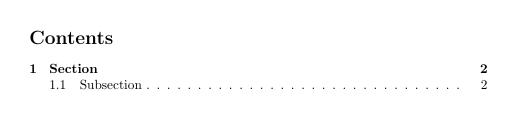
\includegraphics[width=0.70\textwidth]{gambar/Conten}}
	\caption{Hasil Kode Program}
	\label{Hasil Kode Program}
\end{figure}

\vspace{\baselineskip}

\begin{itemize}
	\item Latex
\end{itemize}
\begin{figure}[ht]
	\centerline{\includegraphics[width=0.40\textwidth]{gambar/Latex}}
	\caption{Latex}
	\label{Latex}
\end{figure}

 \par
\vspace{\baselineskip}
Artikel ini menyajikan dasar-dasar untuk membuat dokumen.\par

\hspace*{0.5in}Isi\par

\hspace*{0.5in}1. Perkenalan\par

\hspace*{0.5in}2. Pembukaan dokumen\par

\hspace*{0.5in}3. Menampilkan judul dokumen Anda\par

\hspace*{0.5in}4. Format dasar: abstrak, paragraf dan baris baru\par

\hspace*{0.5in}5. Komentar\par

\hspace*{0.5in}6. Panduan Referensi\par

\vspace{10pt}

	\item {\fontsize{14pt}{14pt}\selectfont \textbf{Pengantar/Perkenalan}}\par
\vspace{\baselineskip}
Mari kita mulai dengan contoh kerja yang paling sederhana:\par

\hspace*{0.5in}$\setminus$ documenkelas $ \{ $arttikel$ \} $\par

\hspace*{0.5in}$\setminus$ begin $ \{ $documen$ \} $\par
\vspace{\baselineskip}

\hspace*{0.5in}Dokumen pertama ini adalah contoh sederhana, dengan no parameter tambahan atau paket \hspace*{0.5in}disertakan.\par

\hspace*{0.5in}$\setminus$ end $ \{ $document$ \} $\par

Baris pertama kode menyatakan jenis dokumen, dalam hal ini adalah sebuah artikel. Kemudian disertakan dalam tag $\setminus$ begin $ \{ $dokumen$ \} $ $\setminus$ end $ \{ $document$ \} $ dan kita harus menulis teks dokumen.\par

\vspace{10pt}
	\item {\fontsize{14pt}{14pt}\selectfont \textbf{Pembukaan Dokumen}}\par
\vspace{\baselineskip}
Pada contoh sebelumnya, teks dimasukkan setelah perintah $\setminus$ begin $ \{ $document$ \} $. Bagian dari file .tex anda sebelum titik ini disebut pendahuluan. Dalam basa-basi anda menentukan jenis dokumen yang anda tulis, bahasa dan beberapa elemen lainnya. Misalnya, pendahuluan dokumen normal akan terlihat seperti ini:\par
\vspace{\baselineskip}
\hspace*{0.5in}$\setminus$ documentclass [12pt, letterpaper] $ \{ $article$ \} $\par
\vspace{\baselineskip}
\hspace*{0.5in}$\setminus$ usepackage [utf8] $ \{ $inputenc$ \} $\par

\hspace*{0.5in}$\setminus$ title $ \{ $Dokumen pertama$ \} $\par
\vspace{\baselineskip}

$\setminus$ author $ \{ $Hubert Farnsworth $\setminus$ thanks $ \{ $didanai oleh tim ShareLaTeX$ \} $$ \} $\par

\hspace*{0.5in}$\setminus$ tanggal $ \{ $September 2017$ \} $\par
\vspace{\baselineskip}
Berikut penjelasan rinci setiap baris:\par
\vspace{\baselineskip}
$\setminus$ documentclass [12pt, letterpaper] $ \{ $article$ \} $\par
\vspace{\baselineskip}
\hspace*{0.5in}Seperti dikatakan sebelumnya, ini mendefinisikan jenis dokumen. Beberapa parameter tambahan di dalam kurung dan dipisahkan koma dapat dilewatkan ke perintah. Pada contoh, parameter tambahan mengatur ukuran font (12pt) dan ukuran kertas (letterpaper). Tentu saja ukuran font lainnya (9pt, 11pt, 12pt) bisa digunakan, ukuran defaultnya adalah 10pt. Sedangkan untuk ukuran kertas, nilai lain yang mungkin adalah a4paper dan legalpaper; \par
\vspace{\baselineskip}
$\setminus$ usepackage [utf8] $ \{ $inputenc$ \} $\par

\hspace*{0.5in}Ini adalah pengkodean untuk dokumen. Dapat dihilangkan atau diubah ke pengkodean lain tapi utf-8 direkomendasikan. Kecuali anda secara khusus memerlukan pengkodean lain, atau jika anda tidak yakin akan hal itu, tambahkan baris ini ke pendahuluan.\par
\vspace{\baselineskip}
Tiga baris berikutnya bersifat deskriptif. Bagaimanapun, Anda bisa melihat deskripsi tentang apa yang sebenarnya mereka lakukan di bagian selanjutnya.\par
\vspace{\baselineskip}
Parameter penting lainnya yang bisa dilewatkan ke perintah documentclass adalah twocolumn jika anda menginginkan teks anda dalam format dua kolom dan dua huruf untuk pencetakan lembar kertas dua sisi.\par
\vspace{\baselineskip}
\vspace{10pt}
	\item {\fontsize{14pt}{14pt}\selectfont \textbf{Menampilkan Judul Dokumen}}\par
\vspace{\baselineskip}
Untuk menampilkan judul dokumen anda, anda harus mendeklarasikan komponennya dalam pembukaan dan kemudian menggunakan beberapa kode tambahan:\par
\vspace{\baselineskip}
\hspace*{0.5in}$\setminus$ documentclass [12pt, letterpaper, twoside] $ \{ $article$ \} $\par

\hspace*{0.5in}$\setminus$ usepackage [utf8] $ \{ $inputenc$ \} $\par

\hspace*{0.5in}$\setminus$ title $ \{ $Dokumen pertama$ \} $\par
\vspace{\baselineskip}
$\setminus$ author $ \{ $Hubert Farnsworth $\setminus$ thanks $ \{ $didanai oleh tim ShareLaTeX$ \} $$ \} $\par
\vspace{\baselineskip}
\hspace*{0.5in}$\setminus$ tanggal $ \{ $September 2017$ \} $\par

\hspace*{0.5in}$\setminus$ begin $ \{ $document$ \} $\par

\hspace*{0.5in}$\setminus$ begin $ \{ $titlepage$ \} $\par

\hspace*{0.5in}$\setminus$ maketitle\par

\hspace*{0.5in}$\setminus$ end $ \{ $titlepage$ \} $\par
\vspace{\baselineskip}
Dalam dokumen ini ada beberapa paket dan parameter tambahan ditambahkan. Ada paket encoding sebuah parameter pageize dan fontsize.\par

\hspace*{0.5in}$\setminus$ end $ \{ $document$ \} $\par

Ada satu blok dengan tiga baris dalam basa-basi yang menentukan informasi apa yang akan dimasukkan ke dalam halaman judul.\par

\hspace*{0.5in}$\setminus$ title $ \{ $Dokumen pertama$ \} $\par

\hspace*{0.5in}Inilah judulnya.\par

\hspace*{0.5in}$\setminus$ author $ \{ $Hubert Farnsworth$ \} $\par

Di sini anda memasukkan nama Pengarang, dan sebagai parameter opsional, anda dapat menambahkan perintah berikutnya:\par
\vspace{\baselineskip}
\hspace*{0.5in}$\setminus$thanks\par

\hspace*{0.5in}$\setminus$ tanggal $ \{ $September 2017$ \} $\par

Anda dapat memasukkan tanggal secara manual atau menggunakan perintah $\setminus$ hari ini sehingga tanggal akan diperbarui secara otomatis pada saat anda mengkompilasi dokumen. \par
\vspace{\baselineskip}
\hspace*{0.5in}$\setminus$ begin $ \{ $titlepage$ \} $ $\setminus$ end $ \{ $titlepage$ \} $\par

Ini menyatakan lingkungan, blok kode dengan perilaku tertentu tergantung pada jenisnya. Dalam hal ini apapun yang anda sertakan di lingkungan judul halaman ini akan muncul di halaman pertama dokumen anda.\par
\vspace{\baselineskip}
\hspace*{0.5in}$\setminus$ maketitle\par

Perintah ini akan mencetak judul, penulis dan tanggal dalam format yang ditunjukkan. Jika tidak tertutup dalam lingkungan judul halaman, dokumen itu akan ditampilkan di awal dokumen, di atas baris pertama.\hspace*{0.5in}\par
\vspace{\baselineskip}
\vspace{10pt}
	\item {\fontsize{14pt}{14pt}\selectfont \textbf{Format Dasar: Abstrak, Paragraf dan Baris Baru}}\par
\vspace{\baselineskip}
Semua yang termasuk dalam perintah $\setminus$ begin $ \{ $document$ \} $ $\setminus$ end $ \{ $document$ \} $ akan diberikan dalam dokumen akhir.\par
\vspace{\baselineskip}
\hspace*{0.5in}$\setminus$ begin $ \{ $document$ \} $\par

\hspace*{0.5in}$\setminus$ begin $ \{ $abstract$ \} $\par
\vspace{\baselineskip}
\hspace*{0.5in}Ini adalah paragraf sederhana di awal dokumen. Pengantar singkat tentang subjek utama.\par
\vspace{\baselineskip}
\hspace*{0.5in}$\setminus$ end $ \{ $abstrak$ \} $\par

Dalam dokumen ini ada beberapa paket dan parameter tambahan ditambahkan. Ada paket encoding sebuah parameter pageize dan fontsize. Baris ini akan memulai Paragraf kedua. Dan saya bisa rem $\setminus$ $\setminus$ the garis $\setminus$$\setminus$ dan lanjutkan di baris baru.\par
\vspace{\baselineskip}
\hspace*{0.5in}$\setminus$ end $ \{ $document$ \} $\par

Dalam dokumen ilmiah, ini adalah praktik umum untuk menyertakan ikhtisar singkat pokok utama makalah ini. Di LATEX ada lingkungan abstrak untuk ini. Lingkungan abstrak akan memasukkan teks dalam format khusus di bagian atas dokumen anda.\par
\vspace{\baselineskip}
Saat menulis isi dokumen anda, jika anda perlu memulai paragraf baru anda harus menekan tombol "Enter" dua kali (untuk memasukkan baris kosong ganda). Perhatikan bahwa paragraf memiliki spasi putih sebelum baris pertama.\par
\vspace{\baselineskip}
Untuk memulai baris baru tanpa benar-benar memulai paragraf baru masukkan titik putus, ini bisa dilakukan oleh $\setminus$$\setminus$ (garis miring terbalik ganda) atau perintah $\setminus$ new line.\par
\vspace{\baselineskip}
\vspace{10pt}
	\item {\fontsize{14pt}{14pt}\selectfont \textbf{Komentar}}\par
\vspace{\baselineskip}
Terkadang perlu menambahkan komentar ke kode LATEX agar mudah dibaca. Ini sangat mudah, beri$\%$ sebelum komentar dan LATEX akan mengabaikan teks itu.\par
\begin{verbatim}

\documentclass \{article} 

\usepackage [utf8] {inputenc} % kodifikasi dokumen

\usepackage {comment} 

Di sini mulai isi dokumen

\begin {document}

\end{verbatim}

\hspace*{0.5in}Dokumen ini berisi banyak komentar, bukan dari mereka akan tetapi muncul disini, hanya teks ini saja. Dokumen ini berisi banyak komentar, bukan dari mereka akan tetapi muncul disini, hanya teks ini saja.\par

\hspace*{0.5in}$\setminus$ begin $ \{ $comment$ \} $\par

\hspace*{0.5in}Teks ini tidak akan muncul dalam pdf yang dikompilasi ini hanya komentar multi-line Misalnya, komentari slow-rendering sambil mengerjakan draft.\par

\hspace*{0.5in}$\setminus$ end $ \{ $comment$ \} $\par

\hspace*{0.5in}$\setminus$ end $ \{ $document$ \} $\par
\vspace{\baselineskip}
Pada bagian terakhir dari contoh, Anda dapat melihat lingkungan komentar, ini membantu dalam komentar multi-baris dan bukan menempatkan$\%$ di awal setiap baris. Agar ini bisa berhasil, Anda harus menambahkan baris berikutnya:\par
\vspace{\baselineskip}
\hspace*{0.64in}$\setminus$usepackage$ \{ $comment$ \} $\par

Simbol$\%$ adalah karakter reserved, jika Anda benar-benar membutuhkan simbol ini untuk dicetak dalam dokumen Anda, gunakan $\setminus$$\%$.\par
\vspace{\baselineskip}
\vspace{10pt}
	\item {\fontsize{14pt}{14pt}\selectfont \textbf{Panduan Referensi}}\par
\vspace{\baselineskip}
Jenis dokumen tersedia dalam perintah $\setminus$ documentclass.\par
\vspace{\baselineskip}
Tipe dokumen\hspace*{0.5in}Deskripsi\hspace*{0.5in}\par

-Artikel\hspace*{0.5in}-Dokumen pendek dan artikel yang paling umum digunakan.\par

-Laporan\hspace*{0.5in}-Untuk dokumen dan disertasi yang lebih panjang.\par

-Buku\hspace*{0.6in}-Untuk menulis buku\par

-Surat\hspace*{0.6in}-Untuk surat berbagai macam\hspace*{0.5in}\par

-Slide\hspace*{0.6in}-Untuk slide, namun jarang digunakan\par

-Beamer\hspace*{0.5in}-Lihat dokumentasi beamer untuk deskripsi yang lebih baik\par
\vspace{\baselineskip}
Karakter yang dilindungi\par
\vspace{\baselineskip}
Karakter simbol berikut dicadangkan oleh LATEX karena mereka mengenalkan perintah dan memiliki arti khusus.\par

$\#$ $\$$$\%$ $ \string^ $ $\&$ $ \_ $ $ \{ $$ \} $ $ \sim $ $\setminus$\par

\vspace{10pt}
	\subsection{Paragraf Baru}

Untuk memulai paragraf baru di LATEX, seperti yang dikatakan sebelumnya, Anda harus membiarkan baris kosong di antaranya. Ada cara lain untuk memulai paragraf baru, lihat cuplikan kode berikut.\par
\vspace{\baselineskip}
Ini teks di paragraf pertama. Ini teksnya terlebih dahulu. Ini adalah teks di paragraf pertama. $\setminus$par\par
\vspace{\baselineskip}
Ini adalah teks dalam paragraf kedua. Ini adalah teks kedua. Ini adalah teks dalam paragraf kedua.\par

Seperti yang bisa anda lihat, perintah $\setminus$ par juga untuk memulai paragraf baru.\par

\vspace{10pt}
	\subsection{Paragraf Alignment (Pembenaran Teks)}

Paragraf di LaTeX sepenuhnya dibenarkan, yaitu dengan margin kiri dan kanan. Jika anda ingin mengubah sebuah paragraf, LATEX memiliki tiga lingkungan : center, flushleft dan flushright.\par
\vspace{\baselineskip}
\hspace*{0.5in}$\setminus$ begin $ \{ $flushleft$ \} $\par

`` LaTeX adalah sistem persiapan dokumen dan markup dokumen bahasa. \par
\vspace{\baselineskip}
LaTeX menggunakan program typesetting TeX untuk pemformatan outputnya, dan ditulis sendiri dalam bahasa makro TeX.\par
\vspace{\baselineskip}
LaTeX bukan nama program pengeditan tertentu, namun merujuk ke konvensi pengkodean atau penandaan yang digunakan dalam dokumen LaTeX ".\par

\hspace*{0.5in}$\setminus$ end $ \{ $flushleft$ \} $\par
\vspace{\baselineskip}
Flushleft kiri-membenarkan paragraf. Untuk right-justify gunakan flushright sebagai gantinya.\par
\vspace{\baselineskip}
Tulisan yang disebutkan di atas didasarkan pada perintah saklar: $\setminus$ raggedright (setara dengan flushleft), $\setminus$ raggedleft (setara dengan flushright) dan keterpusatan (setara dengan pusat). \par
\vspace{\baselineskip}
Perintah switch mengalihkan penyelarasan dari titik di mana ia dimasukkan ke bagian akhir dokumen, kecuali jika ada perintah saklar lain yang dimasukkan.\par

\vspace{10pt}
	\subsection{Paragraf Indentasi}

Secara default, LATEX tidak menyertakan paragraf pertama dari sebuah bagian. Ukuran indentasi paragraf berikutnya ditentukan oleh parameter. \par

\hspace*{0.5in}$\setminus$ setlength $ \{ $$\setminus$ parindent$ \} $ $ \{ $10ex$ \} $\par
\vspace{\baselineskip}
\vspace{\baselineskip}
Ini teks di paragraf pertama. Ini teksnya terlebih dahulu. Ini teks di paragraf pertama. $\setminus$par\par
\vspace{\baselineskip}
\hspace*{0.5in}$\setminus$ noindent$\%$ Paragraf berikutnya tidak menjorok\par
\vspace{\baselineskip}
Ini teks di paragraf kedua. Ini teks kedua. Ini teks dalam paragraf kedua.\par
\vspace{\baselineskip}
Panjang default parameter ini ditentukan oleh kelas dokumen yang digunakan. Hal ini memungkinkan untuk mengubah ukuran indent paragraf dengan menggunakan perintah $\setminus$ setlength. Pada paragraf $\setminus$ setlength $ \{ $$\setminus$ parindent$ \} $ $ \{ $10ex$ \} $ akan menjorok 10ex (sebuah "ex" sama dengan panjang "x" pada font saat ini)\par
\vspace{\baselineskip}
Jika anda ingin membuat paragraf non-indentasi, anda dapat menggunakan perintah $\setminus$ noindent pada awal paragraf.\par
\vspace{\baselineskip}
Jika anda ingin indentasi paragraf yang tidak indentasi, anda bisa menggunakan $\setminus$ indent di atasnya. Perlu dicatat bahwa perintah ini hanya akan berpengaruh bila $\setminus$ parindent tidak diset ke nol.\par
\vspace{\baselineskip}
\vspace{10pt}
	\item {\fontsize{14pt}{14pt}\selectfont \textbf{Jeda Baris}}\par
\vspace{\baselineskip}
Ada lebih dari satu cara untuk memasukkan jeda baris.\par
\vspace{\baselineskip}
\hspace*{0.5in}$\setminus$ documentclass $ \{ $article$ \} $\par

\hspace*{0.5in}$\setminus$ usepackage [utf8] $ \{ $inputenc$ \} $\par

\hspace*{0.5in}$\setminus$ begin $ \{ $document$ \} $\par
\vspace{\baselineskip}
Sesuatu dalam dokumen ini tidak berisi informasi dan tujuannya adalah untuk memberi contoh bagaimana cara menyisipkan spasi dan garis putus. $\setminus$$\setminus$\par
\vspace{\baselineskip}
Jeda baris dimasukkan, disana beberapa perintah tambahan melakukan jeda baris. $\setminus$garis baru. Paragraf ini tidak memberikan informasi apapun. Kami sedang melakukan jeda baris $\setminus$ hfill $\setminus$ break, dan menggabungkan dua perintah\par

\hspace*{0.5in}$\setminus$ end $ \{ $document$ \} $\par

Ada tiga perintah :\par

\hspace*{0.5in}$\setminus$$\setminus$ (dua garis miring terbalik)\par

\hspace*{0.5in}$\setminus$garis baru\par

\hspace*{0.5in}$\setminus$ hfill $\setminus$ break\par
\vspace{\baselineskip}
\vspace{10pt}
	\item {\fontsize{14pt}{14pt}\selectfont \textbf{Jeda Halaman}}\par
\vspace{\baselineskip}
Ada dua perintah untuk memasukkan jeda halaman, clearpage dan newpage. Berikut adalah contoh menggunakan clearpage.\par
\vspace{\baselineskip}
\hspace*{0.5in}$\setminus$ documentclass $ \{ $article$ \} $\par

\hspace*{0.5in}$\setminus$ usepackage [utf8] $ \{ $inputenc$ \} $\par

\hspace*{0.5in}$\setminus$ begin $ \{ $document$ \} $\par
\vspace{\baselineskip}
Sesuatu dalam dokumen ini tidak berisi informasi dan tujuannya adalah untuk memberi contoh bagaimana cara menyisipkan spasi dan garis putus.\par
\vspace{\baselineskip}
Saat jeda baris disisipkan, Beberapa perintah tambahan melakukan jeda baris. $\setminus$garis baru\par
\vspace{\baselineskip}
Paragraf ini tidak memberikan informasi apapun. Kami sedang melakukan jeda baris $\setminus$ hfill $\setminus$ break\par
\vspace{\baselineskip}
Dan menggabungkan dua perintah\par
\vspace{\baselineskip}
\hspace*{0.5in}$\setminus$ begin $ \{ $figure$ \} $\par

\hspace*{0.5in}$\setminus$ centering\par

\hspace*{0.5in}$\setminus$ includegraphics [width = 4cm] $ \{ $singa-logo$ \} $\par

\hspace*{0.5in}$\setminus$ caption $ \{ $ShareLaTeX logo$ \} $\par

\hspace*{0.5in}$\setminus$ end $ \{ $figure$ \} $\par

\hspace*{0.5in}$\setminus$ clearpage\par
\vspace{\baselineskip}
Jika perintah $\setminus$ clearpage digunakan, dan ada elemen mengambang, seperti tabel atau gambar, gambar akan hilang sebelum memulai halaman baru.\par
\vspace{\baselineskip}
Karena jeda halaman dimasukkan sebelum semua gambar ditampilkan, gambar yang tersisa dimasukkan ke halaman kosong sebelum melanjutkan teks di bawah titik brake point.\par
\vspace{\baselineskip}
\hspace*{0.5in}-~ Berikut adalah contoh menggunakan newpage.\par

\hspace*{0.5in}$\setminus$ documentclass $ \{ $article$ \} $\par

\hspace*{0.5in}$\setminus$ usepackage [utf8] $ \{ $inputenc$ \} $ \par

\hspace*{0.5in}$\setminus$ begin $ \{ $document$ \} $\par
\vspace{\baselineskip}
Sesuatu dalam dokumen ini tidak berisi informasi dan tujuannya adalah untuk memberi contoh bagaimana cara menyisipkan spasi dan garis putus. Saat jeda baris disisipkan, Beberapa perintah tambahan melakukan jeda baris. $\setminus$garis baru\par
\vspace{\baselineskip}
Paragraf ini tidak memberikan informasi apapun. Kami sedang melakukan jeda baris $\setminus$ hfill $\setminus$ break Dan menggabungkan dua perintah\par
\vspace{\baselineskip}
\hspace*{0.5in}$\setminus$ begin $ \{ $figure$ \} $\par
\vspace{\baselineskip}
\hspace*{0.5in}$\setminus$ centering\par
\vspace{\baselineskip}
\hspace*{0.5in}$\setminus$ includegraphics [width = 4cm] $ \{ $singa-logo$ \} $\par
\vspace{\baselineskip}
\hspace*{0.5in}$\setminus$ caption $ \{ $ShareLaTeX logo$ \} $\par
\vspace{\baselineskip}
\hspace*{0.5in}$\setminus$ end $ \{ $figure$ \} $ \par
\vspace{\baselineskip}
\hspace*{0.5in}$\setminus$newpage\par
\vspace{\baselineskip}
Dalam hal ini gambar ditempatkan di halaman baru yang mencoba menyesuaikan aliran teks.\par
\vspace{\baselineskip}
\vspace{10pt}
	\item {\fontsize{14pt}{14pt}\selectfont \textbf{Ruang Kosong Horisontal}}\par
\vspace{\baselineskip}
Ruang horisontal dengan panjang yang dapat di tentukan dapat disisipkan dengan $\setminus$ hspace.\par
\vspace{\baselineskip}
Horisontal $\setminus$ hspace $ \{ $1cm$ \} $ spasi dapat dimasukkan secara manual. Berguna untuk mengontrol fine-tuning dalam tata letak gambar.\par

Sisi Kiri Side kanan.\par
\vspace{\baselineskip}
Ada dua perintah yang menyisipkan spasi kosong horisontal pada contoh ini:\par
\vspace{\baselineskip}
\hspace*{0.5in}\textbf{$\setminus$ hspace $ \{ $1cm$ \} $}\par
\vspace{\baselineskip}
Sisipan ruang horisontal yang panjangnya 1cm. Unit LATEX lainnya dapat digunakan dengan perintah ini.\par
\vspace{\baselineskip}
\hspace*{0.5in}\textbf{$\setminus$ hfill}\par
\vspace{\baselineskip}
Sisipkan ruang kosong yang akan merentang sesuai untuk mengisi ruang yang tersedia.\par
\vspace{\baselineskip}
Perintah $\setminus$ hrulefill dan $\setminus$ dotfill melakukan hal yang sama dengan $\setminus$ hfill tapi bukan spasi kosong yang mereka masukkan melainkan ruang horizontal dan satu string titik.\par
\vspace{\baselineskip}
\vspace{10pt}
	\item {\fontsize{14pt}{14pt}\selectfont \textbf{Ruang Kosong Vertikal}}\par
\vspace{\baselineskip}
Ruang kosong vertikal memiliki sintaks yang sama dengan yang horizontal.\par
\vspace{\baselineskip}
\hspace*{0.5in}Teks di bagian atas halaman. Teks di bagian atas halaman.\par

\hspace*{0.5in}Teks di bagian atas halaman. Teks di bagian atas halaman.\par

\hspace*{0.5in}Teks di bagian atas halaman. Teks di bagian atas halaman.\par

\hspace*{0.5in}Teks di bagian atas halaman.\par
\vspace{\baselineskip}
\hspace*{0.5in}$\setminus$ vspace $ \{ $5mm$ \} $$\%$ 5mm ruang vertikal\par

\hspace*{0.5in}Teks ini masih di atas, 5mm di bawah paragraf pertama.\par
\vspace{\baselineskip}
\hspace*{0.5in}$\setminus$ vfill\par

\hspace*{0.5in}Teks di bagian bawah halaman.\par
\vspace{\baselineskip}
Mari kita lihat dua perintah yang menyisipkan ruang kosong vertikal.\par
\vspace{\baselineskip}
\textbf{$\setminus$ vspace $ \{ $5mm$ \} $}\par
Sisipan ruang vertikal yang panjangnya 5mm. Unit LATEX lainnya dapat digunakan dengan perintah ini.\par
\vspace{\baselineskip}

\textbf{$\setminus$ vfill}\par
Sisipkan ruang kosong yang akan membentang sesuai untuk mengisi ruang vertikal yang ada. Itu sebabnya baris "Teks di bagian bawah halaman." dipindahkan ke bawah, dan sisa ruang terisi.\par
\vspace{\baselineskip}
Ada tiga perintah lain yang biasa digunakan untuk memasukkan spasi kosong vertical.\par
\vspace{\baselineskip}

\textbf{$\setminus$ smallskip}\par
Menambahkan spasi 3pt plus atau minus 1pt tergantung pada faktor lain (tipe dokumen, ruang yang tersedia, dll)\par
\vspace{\baselineskip}
\textbf{$\setminus$ medskip}\par
Menambahkan ruang 6pt plus atau minus 2pt tergantung pada faktor lain (tipe dokumen, ruang yang tersedia, dll)\par
\vspace{\baselineskip}

\textbf{$\setminus$ bigskip}\par
Menambahkan ruang 12pt plus atau minus 4pt tergantung pada faktor lain (tipe dokumen, ruang yang tersedia, dll)\par
\vspace{\baselineskip}
\vspace{10pt}
	\item {\fontsize{14pt}{14pt}\selectfont \textbf{Teks Miring}}\par
\vspace{\baselineskip}
Untuk membuat teks miring sangat mudah, gunakan perintah $\setminus$ textit:\par
\vspace{\baselineskip}
\hspace*{0.5in}Beberapa yang terhebat\par

\hspace*{0.5in}penemuan dalam sains\par

\hspace*{0.5in}dibuat oleh $\setminus$ textit $ \{ $accident$ \} $.\par
\vspace{\baselineskip}
Tulisan accident akan otomatis miring.\par
\vspace{\baselineskip}
\vspace{10pt}
	\item {\fontsize{14pt}{14pt}\selectfont \textbf{Teks Tebal}}\par
Untuk membuat teks tebal gunakan perintah $\setminus$ textbf:\par
\hspace*{0.5in}Beberapa $\setminus$ textbf $ \{ $greatest$ \} $\par

\hspace*{0.5in}penemuan dalam sains\par

\hspace*{0.5in}dibuat secara tidak sengaja.\par
Tulisan greatest akan otomatis tebal.\par

\vspace{10pt}
	\item {\fontsize{14pt}{14pt}\selectfont \textbf{Teks Bergaris Bawah}}\par
\vspace{\baselineskip}
Teks yang digaris bawahi sangat sederhana juga, gunakan perintah $\setminus$ underline:\par
\vspace{\baselineskip}
\hspace*{0.5in}Beberapa yang terhebat\par

\hspace*{0.5in}penemuan dalam $\setminus$ underline $ \{ $science$ \} $\par

\hspace*{0.5in}dibuat secara tidak sengaja.\par
\vspace{\baselineskip}
Tulisan science akan otomatis bergaris bawah.\par
\vspace{\baselineskip}
\vspace{10pt}
	\item {\fontsize{14pt}{14pt}\selectfont \textbf{Pemisahan Kolom}}\par
\vspace{\baselineskip}
Pemisahan kolom ditentukan oleh $\setminus$ columnsep. Lihat contoh di bawah ini:\par
\vspace{\baselineskip}
\hspace*{0.5in}$\setminus$ documentclass $ \{ $article$ \} $\par

\hspace*{0.5in}$\setminus$ usepackage [utf8] $ \{ $inputenc$ \} $\par

\hspace*{0.5in}$\setminus$ usepackage [english] $ \{ $babel$ \} $\par

\hspace*{0.5in}$\setminus$ usepackage $ \{ $multicol$ \} $\par

\hspace*{0.5in}$\setminus$ setlength $ \{ $$\setminus$ columnsep$ \} $ $ \{ $1cm$ \} $\par

\hspace*{0.5in}$\setminus$ begin $ \{ $document$ \} $\par

\hspace*{0.5in}$\setminus$ begin $ \{ $multicols$ \} $ $ \{ $2$ \} $\par

\hspace*{0.5in}[\par
\vspace{\baselineskip}
\hspace*{0.5in}\hspace*{0.5in}$\setminus$ section $ \{ $Bagian Pertama$ \} $\par

\hspace*{0.5in}\hspace*{0.5in}Ini akan berhasil \par

\hspace*{0.5in}]\par
\vspace{\baselineskip}
\hspace*{0.5in}\hspace*{0.5in}Halo, berikut ini beberapa teks tanpa makna. \par
\vspace{\baselineskip}
Jika anda membaca teks ini, anda tidak akan mendapatkan informasi. Sangat?\par

\hspace*{0.5in}$\setminus$ end $ \{ $multicols$ \} $\par

\hspace*{0.5in}$\setminus$ end $ \{ $document$ \} $\par

Di sini, perintah $\setminus$ setlength $ \{ $$\setminus$ columnsep$ \} $ $ \{ $1cm$ \} $ mengatur pemisahan kolom menjadi 1cm. Lihat Panjang di LaTeX untuk daftar unit yang tersedia.\par
\vspace{\baselineskip}
\vspace{\baselineskip}
\vspace{12pt}
\vspace{12pt}
	\item {\fontsize{14pt}{14pt}\selectfont \textbf{Kolom Tidak Seimbang}}
\end{itemize}\par
\vspace{\baselineskip}
\noindent Dalam lingkungan multicols default kolomnya seimbang sehingga masing-masing berisi jumlah teks yang sama. Format default ini bisa diubah oleh multicols lingkungan yang berbintang *:\par

\vspace{\baselineskip}
\noindent \hspace*{0.5in}$\setminus$ begin $ \{ $multicols *$ \} $ $ \{ $3$ \} $\par

\vspace{\baselineskip}
\noindent \hspace*{0.5in}[\par

\noindent \hspace*{0.5in}\hspace*{0.5in}$\setminus$ section $ \{ $Bagian Pertama$ \} $\par


\noindent \hspace*{0.5in}\hspace*{0.5in}Ini akan berhasil\par

\vspace{\baselineskip}
\noindent \hspace*{0.5in}]\par

\vspace{\baselineskip}
\noindent \hspace*{0.5in}\hspace*{0.5in}Halo, berikut ini beberapa teks tanpa makna. \par

\vspace{\baselineskip}
Jika anda membaca teks ini, anda tidak akan mendapatkan informasi. Sangat? \par

\vspace{\baselineskip}
\noindent \hspace*{0.5in}$\setminus$ end $ \{ $multicols *$ \} $\par

\vspace{\baselineskip}
\noindent \hspace*{0.5in}$\setminus$ end $ \{ $document$ \} $\par

\vspace{\baselineskip}
\noindent Dalam hal ini teks dicetak dalam kolom sampai akhir halaman tercapai, maka di lanjutkan di kolom berikutnya dan seterusnya.\par


\chapter{Adding Bibliography}

\begin{itemize}
	\item Menurut Wikipedia \par

LaTeX adalah bahasa markup atau sistem penyiapan dokumen untuk peranti lunak TeX. Tex merupakan program komputer yang digunakan untuk membuat typesetting suatu dokumen, atau membuat formula matematika. LaTeX memungkinkan penulis/penggunanya untuk melakukan typesetting dan mencetak hasil kerjanya dalam bentuk tipografi yag terbaik. Oleh karenanya LaTeX paling banyak digunakan oleh para matematikawan, ilmuwan, insinyur, akademisi, dan profesional lainnya.\par

	\item Secara Umum\par

\hspace*{0.5in}LaTeX adalah word processor (pengolah kata, pembuat dokumen) mirip Microsoft Word. LaTeX lebih cocok digunakan untuk membuat dokumen yang panjang, bukan yang pendek. Dengan begitu, keampuhan LaTeX dapat ditampilkan. LaTeX juga lebih dapat menampilkan kecanggihannya ketika kita menulis scientific document.\par

LATEX adalah alat yang hebat untuk membuat dokumen, ini berdasarkan gagasan wysiwym (what you see is what you mean), idea -> apa yang anda lihat adalah apa yang anda maksud), artinya kita hanya fokus pada isi dokumen saja dan computer yang akan mengurus formatnya. Dengan LATEX sangat mudah untuk membuat bahan yang tampak profesional. \par

\begin{itemize}
	\item Manajemen bibliografi dengan bibtex
\end{itemize}\par


\noindent LATEX mendukung bibliografi, baik membuat referensi dalam dokumen atau menyimpannya dalam file eksternal. Artikel ini menjelaskan bagaimana mengelola bibliografi dengan thebibliography dan sistem BibTeX.\par


\noindent Catatan: Jika Anda memulai dari nol sebaiknya menggunakan biblatex karena paket tersebut menyediakan pelokalan dalam beberapa bahasa, ini dikembangkan secara aktif dan membuat manajemen bibliografi lebih mudah dan fleksibel.\par


\noindent Artikel ini menyajikan dasar-dasar untuk membuat dokumen.\par


\noindent \hspace*{0.5in}Isi\par


\noindent \hspace*{0.5in}1. Perkenalan\par


\noindent \hspace*{0.5in}2 Sistem\par


\noindent \hspace*{0.5in}3 Manajemen bibliografi dengan Bibtex\par


\noindent \hspace*{0.5in}4 Berkas bibliografi\par


\noindent \hspace*{0.5in}5 Menambahkan bibliografi dalam daftar isi\par


\noindent \hspace*{0.5in}6 Panduan Referensi\par


\noindent \hspace*{0.5in}7 Bacaan lebih lanjut\par

\vspace{12pt}
	\item {\fontsize{14pt}{14pt}\selectfont \textbf{Pengantar/Perkenalan}}\par

Pengantar\par

Perintah bibliografi standar di LATEX memiliki sintaks yang sama dengan daftar dan item.$\setminus$begin$ \{ $thebibliography$ \} $$ \{ $9$ \} $\par

\hspace*{0.5in}$\setminus$bibitem$ \{ $latexcompanion$ \} $ \par

\hspace*{0.5in}Michel Goossens, Frank Mittelbach, and Alexander Samarin. \par

\hspace*{0.5in}$\setminus$textit$ \{ $The $\setminus$LaTeX$\setminus$ Companion$ \} $. \par

\hspace*{0.5in}Addison-Wesley, Reading, Massachusetts, 1993.\par

\hspace*{0.5in}$\setminus$bibitem$ \{ $einstein$ \} $ \par

\hspace*{0.5in}Albert Einstein. \par

\hspace*{0.5in}$\setminus$textit$ \{ $Zur Elektrodynamik bewegter K$ \{ $$\setminus$"o$ \} $rper$ \} $. (German) \par

\hspace*{0.5in}[$\setminus$textit$ \{ $On the electrodynamics of moving bodies$ \} $]. \par

\hspace*{0.5in}Annalen der Physik, 322(10):891–921, 1905. \par

\hspace*{0.5in}$\setminus$bibitem$ \{ $knuthwebsite$ \} $ \par

\hspace*{0.5in}Knuth: Computers and Typesetting,\par

\hspace*{0.5in}$\setminus$$\setminus$$\setminus$texttt$ \{ $http://www-cs-faculty.stanford.edu/$\setminus$$ \sim $$ \{ $$ \} $uno/abcde.html$ \} $\par

\hspace*{0.5in}$\setminus$end$ \{ $thebibliography$ \} $\par

Pada thebibliography ini menghasilkan daftar referensi; daftar tersebut akan diberi judul "Referensi" di kelas dokumen artikel, dan "Bibliografi" di kelas buku dan laporan. Parameter di dalam tanda kurung, 9 pada contoh, menunjukkan jumlah entri yang akan ditambahkan; parameter dan ini tidak boleh lebih besar dari 99.\par

Untuk membuat daftar bibliografi, perintah $\setminus$ bibitem ini lah yang digunakan. Parameter di dalam tanda kurung diatur untuk memberi label pada entri tersebut dan nantinya dapat digunakan sebagai pengenal untuk referensi. Setelah penutup, teks dengan nama penulis, judul buku, penerbit dan sebagainya sudah masuk.\par

\vspace{12pt}
	\item {\fontsize{14pt}{14pt}\selectfont \textbf{Sistem Tertanam}}\par

Contoh yang disajikan dalam pendahuluan hanya berisi daftar referensi, contoh berikut menunjukkan bagaimana mengutip entri daftar itu di dalam dokumen.\par

\hspace*{0.5in}$\setminus$begin$ \{ $document$ \} $ \par

\hspace*{0.5in}$\setminus$section$ \{ $First section$ \} $\par

\hspace*{0.5in}This document is an example of $\setminus$texttt$ \{ $thebibliography$ \} $ environment using \par

\hspace*{0.5in}in bibliography management. Three items are cited: $\setminus$textit$ \{ $The $\setminus$LaTeX$\setminus$ Companion$ \} $ \par

\hspace*{0.5in}book $\setminus$cite$ \{ $latexcompanion$ \} $, the Einstein journal paper $\setminus$cite$ \{ $einstein$ \} $, and the \par

\hspace*{0.5in}Donald Knuth's website $\setminus$cite$ \{ $knuthwebsite$ \} $. The $\setminus$LaTeX$\setminus$ related items are\par

\hspace*{0.5in}$\setminus$cite$ \{ $latexcompanion,knuthwebsite$ \} $. \par

\hspace*{0.5in}$\setminus$medskip \par

\hspace*{0.5in}$\setminus$begin$ \{ $thebibliography$ \} $$ \{ $9$ \} $\par

\hspace*{0.5in}$\setminus$bibitem$ \{ $latexcompanion$ \} $ \par

\hspace*{0.5in}Michel Goossens, Frank Mittelbach, and Alexander Samarin. \par

\hspace*{0.5in}$\setminus$textit$ \{ $The $\setminus$LaTeX$\setminus$ Companion$ \} $. \par

\hspace*{0.5in}Addison-Wesley, Reading, Massachusetts, 1993. \par

\hspace*{0.5in}$\setminus$bibitem$ \{ $einstein$ \} $ \par

\hspace*{0.5in}Albert Einstein. \par

\hspace*{0.5in}$\setminus$textit$ \{ $Zur Elektrodynamik bewegter K$ \{ $$\setminus$"o$ \} $rper$ \} $. (German) \par

\hspace*{0.5in}[$\setminus$textit$ \{ $On the electrodynamics of moving bodies$ \} $]. \par

\hspace*{0.5in}Annalen der Physik, 322(10):891–921, 1905. \par

\hspace*{0.5in}$\setminus$bibitem$ \{ $knuthwebsite$ \} $ \par

\hspace*{0.5in}Knuth: Computers and Typesetting,\par

\hspace*{0.5in}$\setminus$$\setminus$$\setminus$texttt$ \{ $http://www-cs-faculty.stanford.edu/$\setminus$$ \sim $$ \{ $$ \} $uno/abcde.html$ \} $\par

\hspace*{0.5in}$\setminus$end$ \{ $thebibliography$ \} $ \par

\hspace*{0.5in}$\setminus$end$ \{ $document$ \} $\par

Perintah $\setminus$ cite masukkan nomor yang sesuai dengan entri bibliografi yang labelnya dilewatkan ke dalam tanda kurung. Sebagai contoh, output dari $\setminus$ cite $ \{ $einstein$ \} $ adalah [2].\par

\vspace{12pt}
	\item {\fontsize{14pt}{14pt}\selectfont \textbf{Manajemen bibliografi dengan Bibtex}}\par

BibTeX adalah alat manajemen bibliografi yang banyak digunakan di LATEX, dengan BibTeX entri bibliografi disimpan dalam file terpisah dan kemudian diimpor ke dalam dokumen utama.\par

Begitu file bibliografi eksternal diimpor, perintah $\setminus$ cite digunakan seperti pada contoh pendahuluan.\par

\hspace*{0.5in}Ths document is an example of BibTeX using in bibliography management. Three items \par

are cited: $\setminus$textit$ \{ $The $\setminus$LaTeX$\setminus$ Companion$ \} $ book $\setminus$cite$ \{ $latexcompanion$ \} $, the Einstein\par

journal paper $\setminus$cite$ \{ $einstein$ \} $, and the Donald Knuth's website $\setminus$cite$ \{ $knuthwebsite$ \} $. \par

The $\setminus$LaTeX$\setminus$ related items are $\setminus$cite$ \{ $latexcompanion,knuthwebsite$ \} $. \par

\hspace*{0.5in}$\setminus$medskip \par

\hspace*{0.5in}$\setminus$bibliographystyle$ \{ $unsrt$ \} $\par

\hspace*{0.5in}$\setminus$bibliography$ \{ $sample$ \} $\par

Di bawah ini, deskripsi perintah:\par

$\setminus$bibliography$ \{ $sample$ \} $\par

\hspace*{0.5in}Impor berkas BibTeX "sample.bib" untuk menampilkan bibliografi. Untuk mengimpor beberapa file .bib tulis saja koma-dipisahkan di dalam tanda kurung, ekstensi file tidak diperlukan.\par

$\setminus$bibliographystyle$ \{ $unsrt$ \} $\par

Menetapkan gaya bibliografi untuk digunakan dalam dokumen ini. Informasi yang ditampilkan tergantung pada gaya bibliografi yang digunakan, bahkan jika entri tersebut berisi informasi tentang tanggal, penulis, judul, penerbit dan abstrak, gaya yang digunakan hanya bisa mencetak judul dan pengarangnya.\par

$\setminus$cite$ \{ $einstein$ \} $\par

Ini akan mencetak sejumlah teks, tergantung pada gaya bibliografi, untuk referensi entri bibliografi yang labelnya dilewatkan ke komando. Dalam hal ini, label einstein menghasilkan [2].\par

\vspace{12pt}
	\item {\fontsize{14pt}{14pt}\selectfont \textbf{Berkas Bibliografi}}\par

Referensi bibliografi biasanya disimpan dalam file bibliografi yang ekstensi adalah .bib, file ini terdiri dari daftar catatan dan kolom. Setiap catatan bibliografi menyimpan informasi yang relevan untuk satu entri.\par

\hspace*{0.5in}\hspace*{0.5in}@article$ \{ $einstein,\par

~~~ \hspace*{0.5in}author~=~~~~~  "Albert Einstein",\par

~~~ \hspace*{0.5in}title~=~~~~~~  "$ \{ $Zur Elektrodynamik bewegter K$ \{ $$\setminus$"o$ \} $rper$ \} $. ($ \{ $German$ \} $)\par

~~~ \hspace*{0.5in}~~~ [$ \{ $On$ \} $ the electrodynamics of moving bodies]",\par

~~~ \hspace*{0.5in}journal~=~~~~  "Annalen der Physik",\par

~~~ \hspace*{0.5in}volume~=~~~~~  "322",\par

~~~ \hspace*{0.5in}number~=~~~~~  "10",\par

~~~ \hspace*{0.5in}pages~=~~~~~~  "891--921",\par

~~~ \hspace*{0.5in}year~=~~~~~~~  "1905",\par

~~~ \hspace*{0.5in}DOI~=~~~~~~~~  "http://dx.doi.org/10.1002/andp.19053221004"\par

$ \} $\par

 \par

@book$ \{ $latexcompanion,\par

 \hspace*{0.5in}~~ author~~~ = "Michel Goossens and Frank Mittelbach and Alexander Samarin",\par

 \hspace*{0.5in}~~ title~~~~ = "The $\setminus$LaTeX$\setminus$ Companion",\par

 \hspace*{0.5in}~~ year~~~~~ = "1993",\par

 \hspace*{0.5in}~~ publisher = "Addison-Wesley",\par

 \hspace*{0.5in}~~ address~~ = "Reading, Massachusetts"\par

$ \} $\par

 \par

@misc$ \{ $knuthwebsite,\par

 \hspace*{0.5in}~~ author~~~ = "Donald Knuth",\par

 \hspace*{0.5in}~~ title~~~~ = "Knuth: Computers and Typesetting",\par

 \hspace*{0.5in}~~ url$ \sim $~~~~~ = "http://www-cs-faculty.stanford.edu/$\setminus$~$ \{ $$ \} $uno/abcde.html"\par

$ \} $\par

File ini berisi catatan dalam format khusus, misalnya, referensi bibliografi pertama ditentukan oleh:\par

@article$ \{ $...$ \} $\par

Ini adalah baris pertama entri catatan, @artikel menunjukkan jenis entri dan memberi tahu BibTeX bahwa informasi yang tersimpan di sini adalah tentang sebuah artikel. Selain jenis entri yang ditunjukkan pada contoh (artikel, buku dan misc) ada banyak lagi, lihat panduan referensinya.\par

einstein\par

Label einstein ditugaskan untuk entri ini, adalah pengenal yang dapat digunakan untuk merujuk artikel ini ke dalam dokumen.\par

author = "Albert Einstein",\par

Ini adalah bidang pertama dalam daftar bibliografi, yang menunjukkan bahwa penulis artikel ini adalah Albert Einstein. Beberapa bidang yang dipisahkan koma dapat ditambahkan dengan menggunakan nilai kunci sintaks yang sama, misalnya: judul, halaman, tahun, URL, dll. Lihat panduan referensi untuk daftar bidang yang mungkin.\par

Informasi dalam file ini nantinya dapat digunakan dalam dokumen LATEX untuk menyertakan referensi ini, seperti yang ditunjukkan pada subbagian berikutnya.\par

\vspace{12pt}
	\item {\fontsize{14pt}{14pt}\selectfont \textbf{Menambahkan Bibliografi Dalam Daftar Isi}}\par

Ada dua cara untuk memasukkan daftar pustaka dalam daftar isi, baik secara manual menambahkannya atau menggunakan paket tocbibind (disarankan).\par

Untuk menambahkannya secara manual masukkan baris berikut tepat sebelum perintah $\setminus$ begin $ \{ $thebibliography$ \} $ or\par

\hspace*{0.5in}$\setminus$bibliography\par

$\setminus$addcontentsline$ \{ $toc$ \} $$ \{ $chapter$ \} $$ \{ $Bibliography$ \} $\par

for books and reports or\par

$\setminus$addcontentsline$ \{ $toc$ \} $$ \{ $section$ \} $$ \{ $References$ \} $\par

for articles. If you prefer to use tocbibind see the next example.\par

$\setminus$documentclass[a4paper,10pt]$ \{ $article$ \} $\par

$\setminus$usepackage[utf8]$ \{ $inputenc$ \} $\par

$\setminus$usepackage[english]$ \{ $babel$ \} $\par

$\setminus$usepackage[nottoc]$ \{ $tocbibind$ \} $\par

$\setminus$begin$ \{ $document$ \} $\par

$\setminus$tableofcontents\par

$\setminus$section$ \{ $First Section$ \} $\par

This document ...\par

$\setminus$bibliographystyle$ \{ $unsrt$ \} $\par

$\setminus$bibliography$ \{ $sample$ \} $\par

$\setminus$end$ \{ $document$ \} $\par

Menambahkan baris\par

$\setminus$ usepackage [nottoc] $ \{ $tocbibind$ \} $\par

ke pendahuluan akan mencetak "Referensi" atau "Bibliografi" dalam daftar isi, tergantung pada jenis dokumennya. Hati-hati, itu juga akan menambahkan elemen lain seperti Index, Glossary dan daftar Listing ke daftar isi. Untuk informasi lebih lanjut lihat [dokumentasi paket tocbibind].\par

\vspace{12pt}
	\item {\fontsize{14pt}{14pt}\selectfont \textbf{Panduan Referensi}}\par

\begin{itemize}
	\item Tipe entri standar
\end{itemize}\par


artikel\par




Artikel dari majalah atau jurnal\par




Book\par




Sebuah buku terbitan\par




buku kecil\par




Sebuah karya yang dicetak namun tidak memiliki penerbit atau lembaga sponsor\par




konferensi\par




Sebuah artikel dalam sebuah proses konferensi\par




inbook\par




Bagian dari sebuah buku (bagian, bab dan sebagainya)\par




incollection\par




Bagian dari buku yang memiliki judul sendiri\par




inproceedings\par




Sebuah artikel dalam sebuah proses konferensi\par




manual\par




Dokumentasi teknis\par




masterthesis\par




Sebuah tesis Master\par




misc\par




Sesuatu yang tidak sesuai dengan jenis lainnya\par




phdthesis\par




Sebuah tesis PhD\par




proses\par




Sama seperti konferensi\par




techreport\par




Laporan diterbitkan oleh sebuah institusi\par




tidak dipublikasikan\par




Dokumen tidak dipublikasikan secara formal, dengan penulis dan judul\par



\begin{itemize}
	\item Bidang yang paling umum digunakan di BibTeX\hspace*{0.5in}\par

\hspace*{0.5in}- alamat\hspace*{0.5in}\hspace*{0.5in}- penulis\hspace*{0.5in}\hspace*{0.5in}- daftar\par

\hspace*{0.5in}- judul\hspace*{0.5in}\hspace*{0.5in}- buku judul\hspace*{0.5in}\hspace*{0.5in}- crossref\par

\hspace*{0.5in}- lembaga\hspace*{0.5in}\hspace*{0.5in}- editor\hspace*{0.5in}\hspace*{0.5in}- edisi\par

\hspace*{0.5in}- bulan\hspace*{0.5in}\hspace*{0.5in}- kunci \hspace*{0.5in}\hspace*{0.5in}- jurnal\par

\hspace*{0.5in}- perhatikan\hspace*{0.5in}\hspace*{0.5in}- nomor\hspace*{0.5in}\hspace*{0.5in}- organisasi\par

\hspace*{0.5in}- halaman\hspace*{0.5in}\hspace*{0.5in}- penerbit\hspace*{0.5in}\hspace*{0.5in}- sekolah\par

\hspace*{0.5in}- jenis\hspace*{0.5in}\hspace*{0.5in}- judul\hspace*{0.5in}\hspace*{0.5in}- seri\par

\hspace*{0.5in}- URL\hspace*{0.5in}\hspace*{0.5in}- tahun\hspace*{0.5in}\hspace*{0.5in}- volume\par

\hspace*{0.5in}- ISBN\hspace*{0.5in}\hspace*{0.5in}- ISSN\hspace*{0.5in}\hspace*{0.5in}- LCCN\par

\hspace*{0.5in}- harga\hspace*{0.5in}\hspace*{0.5in}- kata\hspace*{0.5in}\hspace*{0.5in}- kunci abstrak\par

\hspace*{0.5in}- isi\hspace*{0.5in}\hspace*{0.5in}- hak\hspace*{0.5in}\hspace*{0.5in}- cipta\par

	\item {\fontsize{14pt}{14pt}\selectfont \textbf{Gaya Bibliografi Bibtex}}\par

Dua perintah berikutnya adalah perintah yang mengatur gaya bibliografi dan mengimpor file bibliografi. Lihat manajemen bibliografi dengan bibtex untuk informasi lebih lanjut. \par

$\setminus$bibliographystyle$ \{ $stylename$ \} $\par

~ \hspace*{0.5in}$\setminus$bibliography$ \{ $bibfile$ \} $\par

dimana bibfile adalah nama bibliografi. File bib tanpa ekstensi dan stylename\par

\vspace{12pt}
	\item {\fontsize{14pt}{14pt}\selectfont \textbf{Manajemen Bibliografi Dengan Natbib}}\par

Ketika membahas manajemen bibliografi di LATEX, program natbib adalah alternatif yang digunakan di beberapa jurnal. Program ini tidak aktif dikembangkan, namun sangat stabil dan banyak digunakan. Artikel ini menjelaskan bagaimana menggunakan natbib untuk memformat dan mengutip sumber bibliografi.\par

Catatan: Jika Anda memulai dari nol sebaiknya menggunakan biblatex karena paket tersebut menyediakan pelokalan dalam beberapa bahasa, ini dikembangkan secara aktif dan membuat manajemen bibliografi lebih mudah dan fleksibel.\par

	\item {\fontsize{14pt}{14pt}\selectfont \textbf{Penggunaan Dasar}}\par

Contoh kerja sederhana ditunjukkan pada introduksi, ada lebih banyak perintah yang berhubungan dengan kepustakaan yang tersedia.\par

\hspace*{0.5in}$\setminus$documentclass$ \{ $article$ \} $\par

$\setminus$usepackage[utf8]$ \{ $inputenc$ \} $\par

$\setminus$usepackage[english]$ \{ $babel$ \} $\par

$\setminus$usepackage[square,numbers]$ \{ $natbib$ \} $\par

$\setminus$bibliographystyle$ \{ $abbrvnat$ \} $\par

$\setminus$title$ \{ $Bibliography management: $\setminus$texttt$ \{ $natbib$ \} $ package$ \} $\par

$\setminus$author$ \{ $Share$\setminus$LaTeX$ \} $\par

$\setminus$date $ \{ $ $ \} $\par

$\setminus$begin$ \{ $document$ \} $\par

$\setminus$maketitle\par

This document is an example of $\setminus$texttt$ \{ $natbib$ \} $ package using in bibliography \par

management. Three items are cited: $\setminus$textit$ \{ $The $\setminus$LaTeX$\setminus$ Companion$ \} $ book $\setminus$cite$ \{ $latexcompanion$ \} $, the Einstein journal paper $\setminus$citet$ \{ $einstein$ \} $, and the \par

Donald Knuth's website $\setminus$cite$ \{ $knuthwebsite$ \} $. The $\setminus$LaTeX$\setminus$ related items are\par

$\setminus$cite$ \{ $latexcompanion,knuthwebsite$ \} $. \par

$\setminus$medskip\par

$\setminus$bibliography$ \{ $sample$ \} $\par

$\setminus$end$ \{ $document$ \} $\par

\hspace*{0.5in}
\vspace{12pt}\hspace*{0.5in}Ada beberapa perubahan dalam contoh ini:\par

	\item Pilihan kotak dan angka di $\setminus$ usepackage [kuadrat, angka] $ \{ $natbib$ \} $ memungkinkan kuadrat kurung dan kutipan numerik masing-masing. Lihat panduan referensi untuk daftar opsi paket\par

	\item Gaya abbrvnat digunakan di sini, lihat gaya bibliografi\par

	\item Perintah $\setminus$ citet menambahkan nama pengarang ke dalam tanda kutip, terlepas dari gaya kutipannya.
\end{itemize}\par

	\item {\fontsize{14pt}{14pt}\selectfont \textbf{Manajemen Bibliografi Dengan Biblatex}}\par

Ketika membahas paket manajemen bibliografi, ada tiga pilihan utama di LATEX: bibtex, natbib dan biblatex. Biblatex adalah sebuah program modern untuk memproses informasi bibliografi, menyediakan antarmuka yang lebih mudah dan lebih fleksibel dan lokalisasi bahasa yang lebih baik sehingga dua opsi lainnya. Artikel ini menjelaskan bagaimana menggunakan biblatex untuk mengelola dan memformat bibliografi dalam dokumen LATEX.\par

\vspace{12pt}
	\item {\fontsize{14pt}{14pt}\selectfont \textbf{Menyesuaikan Bibliografi}}\par

Biblatex memungkinkan kustomisasi yang tinggi dari bagian bibliografi dengan sedikit usaha. Disebutkan bahwa beberapa gaya kutipan dan gaya bibliografi tersedia, dan Anda juga bisa membuat yang baru. Pilihan penyesuaian lainnya adalah mengubah judul default dari bagian ~ \par

 $\setminus$documentclass$ \{ $article$ \} $\par

$\setminus$usepackage[utf8]$ \{ $inputenc$ \} $\par

$\setminus$usepackage[english]$ \{ $babel$ \} $\par

$\setminus$usepackage$ \{ $comment$ \} $\par

$\setminus$usepackage[\par

backend=biber,\par

style=alphabetic,\par

sorting=ynt\par

]$ \{ $biblatex$ \} $\par

$\setminus$addbibresource$ \{ $sample.bib$ \} $\par

$\setminus$title$ \{ $Bibliography management: $\setminus$texttt$ \{ $biblatex$ \} $ package$ \} $\par

$\setminus$author$ \{ $Share$\setminus$LaTeX$ \} $\par

$\setminus$date$ \{ $ $ \} $\par

$\setminus$begin$ \{ $document$ \} $\par

$\setminus$maketitle\par

Using $\setminus$texttt$ \{ $biblatex$ \} $ you can display bibliography divided into sections, \par

depending of citation type. \par

Let's cite! The Einstein's journal paper $\setminus$cite$ \{ $einstein$ \} $ and the Dirac's \par

book $\setminus$cite$ \{ $dirac$ \} $ are physics related items. \par

Next, $\setminus$textit$ \{ $The $\setminus$LaTeX$\setminus$ Companion$ \} $ book $\setminus$cite$ \{ $latexcompanion$ \} $, the Donald \par

Knuth's website $\setminus$cite$ \{ $knuthwebsite$ \} $, $\setminus$textit$ \{ $The Comprehensive Tex Archive \par

Network$ \} $ (CTAN) $\setminus$cite$ \{ $ctan$ \} $ are $\setminus$LaTeX$\setminus$ related items; but the others Donald \par

Knuth's items $\setminus$cite$ \{ $knuth-fa,knuth-acp$ \} $ are dedicated to programming. \par

$\setminus$medskip \par

$\setminus$printbibliography[title=$ \{ $Whole bibliography$ \} $] bibliografi.\par

Judul parameter tambahan = $ \{ $Seluruh bibliografi$ \} $ dilewatkan di dalam tanda kurung ke perintah $\setminus$ printbibliography adalah yang mengubah judul.\par

Bibliografi juga dapat dibagi menjadi beberapa bagian berdasarkan filter yang berbeda, misalnya: hanya mencetak referensi dari penulis yang sama, jurnal yang sama atau judul yang serupa. Berikut contohnya.\par

$\setminus$printbibliography[type=article,title=$ \{ $Articles only$ \} $]\par

$\setminus$printbibliography[type=book,title=$ \{ $Books only$ \} $]\par

 \par

$\setminus$printbibliography[keyword=$ \{ $physics$ \} $,title=$ \{ $Physics-related only$ \} $]\par

$\setminus$printbibliography[keyword=$ \{ $latex$ \} $,title=$ \{ $$\setminus$LaTeX-related only$ \} $]\par

Di sini, bibliografi terbagi dalam 4 bagian. Sintaks dari perintah yang digunakan di sini dijelaskan di bawah ini:\par

$\setminus$printbibliography[type=article,title=$ \{ $Articles only$ \} $]\par

Hanya mencetak entri yang jenisnya adalah "artikel", dan menetapkan judul "Artikel saja" untuk bagian ini. Sintaks yang sama bekerja untuk jenis entri lainnya.\par

$\setminus$printbibliography[keyword=$ \{ $physics$ \} $,title=$ \{ $Physics-related only$ \} $]\par

Menyaring entri bibliografi yang menyertakan kata "fisika" di salah satu bidang. Menetapkan judul "hanya terkait Fisika" untuk bagian tersebut.\par

Bibliography sorting options\par

-option\hspace*{0.5in}\hspace*{0.5in}\hspace*{0.5in}-description\par

nty\hspace*{0.5in}\hspace*{0.5in}\hspace*{0.5in}sort by name, title, year\par

nyt\hspace*{0.5in}\hspace*{0.5in}\hspace*{0.5in}sort by name, year, title\par

nyvt\hspace*{0.5in}\hspace*{0.5in}\hspace*{0.5in}sort by name, year, volume, title\par

anyt\hspace*{0.5in}\hspace*{0.5in}\hspace*{0.5in}sort by alphabetic label, name, year, title\par

anyvt\hspace*{0.5in}\hspace*{0.5in}\hspace*{0.5in}sort by alphabetic label, name, year, volume, title\par

ydtn\hspace*{0.5in}\hspace*{0.5in}\hspace*{0.5in}sort by year (descending), name, title\par

none\hspace*{0.5in}\hspace*{0.5in}\hspace*{0.5in}entries are processed in citation order\par

\vspace{12pt}
	\item {\fontsize{14pt}{14pt}\selectfont \textbf{Daftar Isi}}\par

Dalam dokumen LATEX, daftar isi dapat dibuat secara otomatis, dan dimodifikasi agar sesuai dengan gaya tertentu, artikel ini menjelaskan caranya.\par

Untuk membuat daftar isi sangat mudah, perintah $\setminus$ tableofcontents melakukan pekerjaan:\par

\hspace*{0.5in}$\setminus$documentclass$ \{ $article$ \} $\par

$\setminus$usepackage[utf8]$ \{ $inputenc$ \} $\par

$\setminus$title$ \{ $Sections and Chapters$ \} $\par

$\setminus$author$ \{ $Gubert Farnsworth$ \} $\par

$\setminus$date$ \{ $ $ \} $\par

$\setminus$begin$ \{ $document$ \} $\par

$\setminus$maketitle\par

$\setminus$tableofcontents\par

$\setminus$section$ \{ $Introduction$ \} $\par

This is the first section.\par

Lorem~ ipsum~~dolor~~sit~~amet,~~consectetuer  adipiscing  elit.   Etiam~ lobortisfacilisis~sem.  Nullam nec~mi et neque pharetra sollicitudin.  Praesent imperdietmi nec ante. \par

Donec ullamcorper, felis non sodales...\par

$\setminus$addcontentsline$ \{ $toc$ \} $$ \{ $section$ \} $$ \{ $Unnumbered Section$ \} $\par

$\setminus$section*$ \{ $Unnumbered Section$ \} $\par

Lorem ipsum dolor sit amet, consectetuer adipiscing elit. Etiam~lobortis facilisissem.  Nullam nec~mi et neque pharetra sollicitudin.  Praesent imperdiet mi necante...\par

$\setminus$section$ \{ $Second Section$ \} $\par

Lorem ipsum dolor sit amet, consectetuer adipiscing elit. Etiam~lobortis facilisissem.  Nullam nec~mi et neque pharetra sollicitudin.  Praesent imperdiet mi necante...\par

$\setminus$end$ \{ $document$ \} $\par

Bagian, subbagian dan bab disertakan dalam daftar isi. Untuk menambahkan entri secara manual, misalnya bila Anda menginginkan bagian yang tidak terhitung jumlahnya, gunakan perintah $\setminus$ addcontentsline seperti yang ditunjukkan pada contoh.\par

Catatan: Untuk daftar isi agar bekerja dengan baik Anda harus mengkompilasi dokumen dua kali atau menggunakan latexmk -pdf\par

\vspace{12pt}
	\item {\fontsize{14pt}{14pt}\selectfont \textbf{Ubah Judul Daftar Isi}}
\end{itemize}\par


\noindent Judul default untuk daftar isi adalah "Isi", ini bisa diubah menjadi apapun yang Anda butuhkan.\par


\noindent baris $\setminus$ renewcommand * $\setminus$ contentsname $ \{ $Summary$ \} $ akan menulis "Ringkasan" alih-alih nilai default. Jika Anda menggunakan paket babel untuk dukungan bahasa internasional, perintah tersebut harus ditempatkan di dalam tanda kurung.\par


\noindent $\setminus$ addto $\setminus$ capionsenglish $ \{ $$ \} $\par


\noindent Alih-alih bahasa inggris di $\setminus$ captionenglish tuliskan nama bahasa yang Anda tetapkan di babel.\par


\noindent \hspace*{0.5in}$\setminus$documentclass$ \{ $article$ \} $\par

$\setminus$usepackage[utf8]$ \{ $inputenc$ \} $\par

$\setminus$title$ \{ $Sections and Chapters$ \} $\par

$\setminus$author$ \{ $Gubert Farnsworth$ \} $\par

$\setminus$date$ \{ $ $ \} $\par

$\setminus$renewcommand*$\setminus$contentsname$ \{ $Summary$ \} $\par

$\setminus$begin$ \{ $document$ \} $\par

$\setminus$maketitle\par

$\setminus$tableofcontents\par

$\setminus$section$ \{ $Introduction$ \} $\par

This is the first section.\par


Lorem~ ipsum~~dolor~ sit  amet,~~consectetuer~ adipiscing  elit. Etiam~ lobortisfacilisis~sem.  Nullam nec~mi et neque pharetra sollicitudin.  Praesent imperdietmi nec ante. Donec ullamcorper, felis non sodales...\par



$\setminus$addcontentsline$ \{ $toc$ \} $$ \{ $section$ \} $$ \{ $Unnumbered Section$ \} $\par

$\setminus$section*$ \{ $Unnumbered Section$ \} $\par


Lorem ipsum dolor sit amet, consectetuer adipiscing elit. Etiam~lobortis facilisissem.  Nullam nec~mi et neque pharetra sollicitudin.  Praesent imperdiet mi necante...\par



$\setminus$section$ \{ $Second Section$ \} $\par


Lorem ipsum dolor sit amet, consectetuer adipiscing elit. Etiam~lobortis facilisissem.  Nullam nec~mi et neque pharetra sollicitudin.  Praesent imperdiet mi necante...\par




\noindent  \hspace*{0.5in}$\setminus$end$ \{ $document$ \} $\par



\chapter{Adding Footnotes}

\vspace{\baselineskip}
\section{penjelasan tentang catatan kaki dan fungsinya}

\vspace{\baselineskip}
Yang dimaksud dengan catatan kaki adalah daftar keterangan khusus yang ditulis pada bagian paling bawah disetiap lembaran akhir bab karya ilmiah (makalah, skripsi, tesis dll). Atau catatan kaki merupakan keterangan refrensi yang ditempatkan pada kaki tulisan atau teks karya ilmiah.\par

\vspace{\baselineskip}
Berikut ini beberapa fungsi dari catatan kaki yang diantaranya seperti:\par


\vspace{\baselineskip}
\noindent Catatan kaki berfungsi untuk memberikan keterangan dan penjelasan tentang sumber dari kutipan penyusunan daftar bacaan pada karya ilmiah supaya dapat dimengerti oleh pembaca.\par

\vspace{\baselineskip}
\noindent untuk menghargai sumber kutipan yang dikutip, supaya pembaca karya ilmiah mengetahui sumber kutipan yang digunakan\par

\vspace{\baselineskip}
\noindent Dan untuk menunjukan refrensi lain supaya pembaca karya ilmiah dapat mengetahui ulasan yang lebih jelas mengenai istilah yang digunakan\par

\vspace{\baselineskip}
\subsection{cara penulisan catatan kaki}

\vspace{\baselineskip}
\noindent Bagaimana cara menulis catatan kaki?\par

\vspace{\baselineskip}
Dalam penulisannya, catatan kaki memiliki aturan-aturan yang perlu diperhatikan. Hal-hal tersebut diterapkan supaya dapat dimengerti oleh para pembaca karya ilmiah. Dalam menulis catatan kaki ada beberapa hal yang perlu diperhatikan, yang diantaranya:\par

\begin{itemize}
	\vspace{\baselineskip}
	\item Penulisannya dipisahkan oleh garis yang panjangnya 14 karakter dari margin sebelah kiri dan berjarak 4 spasi dari tulisan atau teks.\par

\vspace{\baselineskip}
	\item Diketik atau ditulis dengan satu spasi.\par

\vspace{\baselineskip}
	\item Harus diberikan nomer.\par

\vspace{\baselineskip}
	\item Nomer pada catatan kaki diketik dengan jarak 6 karakter dari margin sebelah kiri.\par

\vspace{\baselineskip}
	\item Kalau catatan kakinya lebih dari satu baris, maka pada baris yang kedua maupun selanjutnya dimulai seperti margin teks yang biasanya tepat pada margin bagian sebelah kiri.\par

\vspace{\baselineskip}
	\item Kalau catatan kakinya lebih dari satu maka jarak antar catatan kaki dengan catatan kaki yang lainnya sama seperti jarak spasi pada teks.\par

\vspace{\baselineskip}
	\item Catatan kaki harus ditulis pada halaman yang sama, jika terlalu panjang lebih baik potong teksnya daripada memotong catatan kaki.\par

\vspace{\baselineskip}
	\item Berjarak 3 centimeter dengan margin bagian bawah, seperti halnya pada aturan teks.\par

\vspace{\baselineskip}
	\item Jika nama pengarang dua sampai tiga orang, maka harus ditulis semuanya. Sedangkan jika nama pengarangnya lebih dari tiga orang maka tulis saja nama pengarang yang pertama lalu dibelakangnya ditulis et.al., atau dkk.\par

\vspace{\baselineskip}
	\item Nama pengarang harus ditulis sesuai nama aslinya, pangkat dan gelar tidak perlu ditulis.\par

\vspace{\baselineskip}
	\item Judul buku atau sumber harus diberi garis bawah, jika diketik dengan komputer maka harus dicetak miring.\par

\vspace{\baselineskip}
Footnotes Merupakan catatan kaki dalam penulisan pada latex \par

\vspace{\baselineskip}
Berikut adalah contoh code latex:\par

\vspace{\baselineskip}
Coding pembuatan catatan kaki\par

\vspace{\baselineskip}
$documentclass$ \{ $article$ \} \par

$begin$ \{ $document$ \} \par

$title$ \{ $google$ \} \par

\vspace{\baselineskip}
Penjelasan syntax yang tadi di pakai adalah sebagai berikut :\par

\vspace{\baselineskip}
$Documenclass$ \{ $article$ \} \par

\vspace{\baselineskip}
	\item Untuk menentukan jenis halaman (kita menggunakan article)\par

$begin$ \{ $document$ \} \par

\vspace{\baselineskip}
	\item Untuk memulai document\par

$title$ \{ $google$ \} \par

\vspace{\baselineskip}
	\item Untuk membuat judul teks, yaitu ‘google’\par

$maketitle$\par

\vspace{\baselineskip}
-Untuk menampilkan judul\par

\vspace{\baselineskip}
$footnote$ \{ $teks$ \} \par

\vspace{\baselineskip}
	\item Untuk membuat catatan kaki tersebut\par

\vspace{\baselineskip}
$end$ \{ $document$ \} \par
	\item Untuk mengakhiri document\par

\vspace{\baselineskip}
Coding yang akan digunakan sebagai berikut :\par

\vspace{\baselineskip}
Documentclass \{ $article$ \} \par

\vspace{\baselineskip}
Begin \{ $document$ \} \par

\vspace{\baselineskip}
$end$ \{ $document$ \} \par

\vspace{\baselineskip}
Penjelasan syntax yang tadi di gunakan berikut penjelasan nya:\par

\vspace{\baselineskip}
$documenclass$ \{ $article$ \} \par

\vspace{\baselineskip}
	\item Untuk menentukan jenis halaman\par


$begin$ \{ $document$ \} \par

	\item Untuk memulai dokumen\par

\vspace{\baselineskip}
$flushleft$\par

	\item Untuk penulisan rata kiri\par

\vspace{\baselineskip}
$\$$\par

	\item Untuk syarat penulisan rumus (di awal dan di akhir)\par

\vspace{\baselineskip}
$ \string^ $\par

	\item Untuk penulisan pangkat atau superscript\par

\vspace{\baselineskip}
$ \_ $\par

	\item Untuk penulisan index atau subscript\par

\vspace{\baselineskip}
$frac$\par

	\item Untuk menuliskan pecahan\par

\vspace{\baselineskip}
$pm$\par

-Untuk penulisan plus minus\par

\vspace{\baselineskip}
$sqrt$\par

	\item Untuk penulisan akar\par

\vspace{\baselineskip}
$alpha$\par

\vspace{\baselineskip}
	\item Untuk menuliskan symbol alpa
	
\end{itemize}\par

\vspace{\baselineskip}
Jadi xxx itu adalah penulisan kata-kata sendiri jadi isi sendiri agar tidak ditiru atau di modif sembarangan\par

\vspace{\baselineskip}
\noindent Penjelasan tentang footnote atau pembuatan catatan kaki\par

\vspace{\baselineskip}
Verbatim berfungsi untuk membuat kalimat atau karakter yang di tulis\par

\vspace{\baselineskip}
Table berfungsi membuat table\par

\vspace{\baselineskip}
4.6.1 pembuatan list dan item pembuatan daftar berurutan untuk membuat daftar yang berurutan\par

\vspace{\baselineskip}
Jadi penulisan yang tepat yaitu menggunakan\par

\vspace{\baselineskip}
Documentclass[12pt,a4paper,oneside,bahasa,dvips] book atau begin document halo, jadi penjelasan nya kita akan membuat dokumen dengan ukuran kertas a4, selanjutnya buku tersebut akan ditampilkan kedalam bahasa Indonesia, dan daftar tersebut akan di susun secara otomatis pada awal dokumen\par


\vspace{\baselineskip}
\noindent 1.4 Hal penting untuk mengatur dokumen atau margin\par

\vspace{\baselineskip}
keterangan yang akan di terangkan berupa\par


\vspace{\baselineskip}
\noindent documentclass\par


\begin{itemize}

\vspace{\baselineskip}
	\item tadi yang menentukan dokumen apa yang akan anda buat\par

\vspace{\baselineskip}
12pt\par

	\item Ukuran huruf\par

\vspace{\baselineskip}
A4paper\par

	\item Jenis\par

\vspace{\baselineskip}
Titlepage\par

	\item Judul terpisah dengan isi\par

\vspace{\baselineskip}
Notitlepage\par

	\item Judul tidak terpisah dengan isi\par

\vspace{\baselineskip}
Oneside\par

	\item Satu sisi\par

\vspace{\baselineskip}
Twocolomn\par

	\item Tampilan dokumen\par

\vspace{\baselineskip}
Bahasa\par

	\item Bahasa Indonesia
	\vspace{\baselineskip}
	
\end{itemize}\par

\vspace{\baselineskip}
\noindent 1.5 Setelah melakuka itu kita bisa membuat sebuah title\par

\vspace{\baselineskip}
\noindent $title$ \{ a \} \par

\vspace{\baselineskip}
\noindent maketitle\par

\begin{itemize}
	
	\vspace{\baselineskip}
	\item Jadi yang di dalam kurung itu isi sesuia yang di inginkan kalian\par

\vspace{\baselineskip}
1.6 Membuat author\par

\vspace{\baselineskip}
	\item Letakan kode nya diantara title dan maketitle lalu isi dalam kurung tersebut nama pengarang\par

\vspace{\baselineskip}
$author$ \{ a \} \par

	\item Jadi sebenernya author juga berfungsi dengan enter\par

\vspace{\baselineskip}
1.7 Cara membuat judul\par
\begin{verbatim}
	
part l

section l  

subsection  l 
\end{verbatim}

\vspace{\baselineskip}
	\item Dalam kurung isi dengan judul yang di buat\par

\vspace{\baselineskip}
1.8 Penomoran dokumen\par
\begin{verbatim}

begin \{ enumerate \}

item

item

item

$end$ \{ enumerate \}
\end{verbatim}

\vspace{\baselineskip}
1.9 Bila ingin menambahkan footnote bisa ditambahkan code nya\par

\vspace{\baselineskip}
footnote \{ l \} \par

\vspace{\baselineskip}
	\item Contoh lain dari footnote adalah\par

$footnote$ \{ $…$ \} \par

\vspace{\baselineskip}
	\item Kurung tersebut bisa di isi dan di sesuaikan dengan keinginan masing masing\par

$documentclass$ \{ $article$ \} \par

$begin$ \{ $document$ \} \par

Bla bla bla.$footnote$ \{ $ini footnote.$ \} \par

$end$ \{ $document$ \} \par

\vspace{\baselineskip}
Maka hasil nya akan bla bla bla ada pangkatnya di atas kata kata blabla bla tersebut\par

\vspace{\baselineskip}
Ini adalah penulisan dan penjelasan catatn kaki tujuan nya agar pembaca mengetahui fungsi dari catatan kaki dalam pembuatan karya ilmiah\par
\begin{itemize}
	\item isal1
\end{itemize}
\begin{figure}[ht]
	\centerline{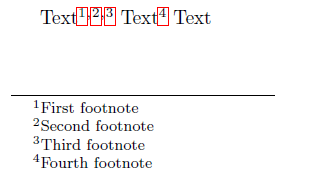
\includegraphics[width=0.70\textwidth]{gambar/isal1}}
	\caption{penulisan catatan kaki}
	\label{catatan kaki}
\end{figure}
\subsection{kesalahan dalam penulisan catatan kaki menurut kaidah EYD}
\begin{itemize}
	
	\vspace{\baselineskip}
	\item Eveline Siregar dan Hartini Nara, Teori Belajar Dan Pembelajaran, (Bogor:Ghalia Indonesia, 2010)hal 4
\end{itemize} 

\vspace{\baselineskip}
Perbaikan nya seperti ini\par

\vspace{\baselineskip}
Eveline Siregar dan Hartini Nara, Teori Belajar Dan Pembelajaran (bogor: Ghalia Indonesia. 2010),hlm.4.\par

\vspace{\baselineskip}
Kesalahan:\par
\begin{itemize}
	\vspace{\baselineskip}
	\item Taniredja, Tukiran, Efi, dan Sri, Metode-metode pembelajaran inovatif (Bandung:Alfabeta.2011)hal 23
\end{itemize}

\vspace{\baselineskip}
Perbaikan nya seperti ini\par

\vspace{\baselineskip}
TAniredja, Tukiran ,Efi, dan Sri, Metode-metode pembelajaran inovatif\par

(Bandung:Alfabeta,2011), hlm 23.\par

\vspace{\baselineskip}
Jadi pengertian catatan kaki adalah keterangan-keterangan atas teks/naskah/tulisna yang ditempatkan pada kaki halaman tulisan yang bersangkutan\par

(keraf, 2004:218)\par

\vspace{\baselineskip}
2.2 Tujuan nya adalah\par

\vspace{\baselineskip}
Catatan kaki tidak hanya sebagai bukti bahwa tulisan kita berasal dari buku lain melainkan ada banyak tujuannya antara lain:\par

\vspace{\baselineskip}
	\item Pembuktian menunjukan tempat/sumber bahwa yang disebutkan pada tulisan telah dibuktikan orang lain.\par

\vspace{\baselineskip}
	\item Memberi apresiasi penghargaan, rasa terima kasih pada orang yang telah dikutipnya\par

\vspace{\baselineskip}
	\item Menyampaikan keterangan tambahan memperkuat uraian di luar persoaalan dalam teks, biasanya berupa: inti cerita, informasi tambahan
\end{itemize}\par

\vspace{\baselineskip}
\noindent Merujuk bagian lain dalam tulisan dalam tulisan referensi melihat bagian lain dalam tulisannya, biasanya dengan singkatan-singkatan tertentu\par

\vspace{\baselineskip}
\noindent Contoh lain yang bisa kita lihat adalah\par

\vspace{\baselineskip}
\noindent Cara penulisan atau pencantuman nama\par


\begin{itemize}
\vspace{\baselineskip}
	\item pengarang (tanpa dibalik)\par

\vspace{\baselineskip}
Judul(dicetak miring atau jika ditulis tangan digaris bawah)\par

\vspace{\baselineskip}
Data publikasi (meliputi kota terbit kemudian titik dua (:) kemudian penerbit koma (,) tahun terbit\par

\vspace{\baselineskip}
Nomor halaman\par

\vspace{\baselineskip}
2.3 Atau bisa disebut juga keterangan atas teks karangan yang di tempatkan pada kaki halaman karangan yang bersangkutan (Gorys Keraf, 1994:193). Catatan kaki dapat berupa rujukan bahan penulisan yang dijadikan sumber dan dapat pula berupa keterangan tambahan.\par

\vspace{\baselineskip}
Fungsinya berupa\par

\vspace{\baselineskip}
	\item Catatan kaki yang berupa referensi\par

\vspace{\baselineskip}
	\item Fungsi akademis\par

\vspace{\baselineskip}
	\item Memberikan dukungan argumentasi atau pembuktian\par

\vspace{\baselineskip}
	\item Pembuktian(rujukan) kutipan naskah\par

\vspace{\baselineskip}
	\item Memperluas makna informasi bahasan dalam naskah\par

\vspace{\baselineskip}
	\item Kebenerana fakta\par

\vspace{\baselineskip}
	\item Kualitas karangan\par

\vspace{\baselineskip}
	\item Penilaian sumber data\par

\vspace{\baselineskip}
	\item Pembedaan data pusaka dan keterangan tambahan\par

\vspace{\baselineskip}
	\item Mencegah pengulangan data pustaka\par

\vspace{\baselineskip}
	\item Memudahkan peninjauan penggunaan referensi\par

\vspace{\baselineskip}
	\item Penyunting data pustaka\par

\vspace{\baselineskip}
	\item Menunjukan kualitas kecerdasan akademis penulisan\par

\vspace{\baselineskip}
	\item Etika atau moral\par

\vspace{\baselineskip}
	\item Pengakuan dan penghargaan kepada penulis\par

\vspace{\baselineskip}
	\item Kualitas ilmiah\par

\vspace{\baselineskip}
	\item Kecermatan lebih akurat\par

\vspace{\baselineskip}
	\item Intelektual bukan plagiat\par

\vspace{\baselineskip}
	\item Kesantunan akademis penulisan\par

\vspace{\baselineskip}
	\item Tempat catatan kaki\par

\vspace{\baselineskip}
	\item Uraian pada halaman yang sama pada bagian bawah digunakan dalam skripsi dan lain lain\par

\vspace{\baselineskip}
	\item Uraian catatan bab terakhir untuk karangan popular\par

\vspace{\baselineskip}
	\item Penempatan catatan kaki harus konsisten. Misalnya, penempatan catatan kaki pada kaki halaman pertama. Penempatan ini dilakukan seterusnya dengan cara yang sama sampai dengan halaman terakhir.
\end{itemize}\par

\vspace{\baselineskip}
\noindent 2.4  Penulisan catatan kaki\par

\begin{itemize}
	\vspace{\baselineskip}
	\item Dipisah tiga sepasi dari naskah yang sama\par

\vspace{\baselineskip}
	\item Antaracatatan kaki dipisahkan dengan satu spasi\par

\vspace{\baselineskip}
	\item Diketik sejajar dengan margin
\end{itemize}\par

\vspace{\baselineskip}
\noindent Itu adalah cara tips untuk mengetahui catatan kaki dan bagaimana penerapan pada latex tersebut maka ikuti langkah diatas maka akan kalian ketahui hasilnya selain itu pembelajaran diatas didapatkan di halaman internet untuk pemahaman lebih jelasnya bisa buka halaman cara penulisan bahasaindonesia di browser pembaca terimakasih\par


\chapter{Create Tables with Latex}

\sloppy

\noindent \begin{center}
	Create Tables With Latex
\end{center}

\noindent 1.1 Tips membuat table pada latex\par


\noindent documentclass[10] \{ $article$ \} \par

\begin{itemize}
	\item Jadi class dokumen ini menggunaka kertas ukuran font 10 dan jenis dokumen nya itu artikel\par

begin \{ $document$ \} \par

	\item Memulai penulisan document\par

begintitle\{ $table$ \} \par

	\item Memulai untuk menggunakan table\par

	\item Karena di dokumen ini membutuhkan table
\end{itemize}\par
\begin{itemize}
	\item Jadi fungsi tabular itu untuk membuat kolom
\end{itemize}\par

\begin{itemize}
	\item Tanda $ \vert $ itu untuk membuat garis kolomnya yang bisa kita tentukan sendiri\par

	\item Dan tanda l itu adalah left
\end{itemize}\par


\noindent Kesimpulan nya semua tulisan berada dikolom itu menggunakan rata kiri\par


\noindent hline\par

\begin{itemize}
	\item Fungsi ini adalah membuat garis sesuai dengan lebar kolom yang kita buat\par

	\item Hline ini juga berfungsi sebagai menentukan berapa baris yang kita mau
\end{itemize}\par
\begin{itemize}
	\item Memasuki baris pertama yang di sebut attribute\par

	\item Attribute ini adalah nama,npm,kelas,jurusan dan semester\par

	\item Textbf ini berfungsi sebagaimembuat tulisan menjadi tebal atau bold\par

	\item Tanda $\&$ ini berguna untuk memisahkan kolom satu dan kolom lain nya
\end{itemize}\par


\noindent hline\par

\begin{itemize}
	\item Berfungsi untuk membuat garis sesuai dengan lebar kolom yang kita buat\par

Garis pertama sudah di buat lalu buat garis kedua\par

Berarti kita masuk baris kedua\par

Faisal akbar ramadhan$\&$1144010$\&$3DTID4$\&$TI$\&$7\par

Dibaris kedua ini tulisan faisal satu kolom dengan nama dan 3dtid4 satu kolom dengan attribute kelas, 1144010 ini berada di kolom npm, ti berada di kolom jurusan dan terakhir 7 adalah kolom untuk semester\par

Selanjutnya isi table dengan cara yang sama dan isi table ini merupakan langkah berikutnya\par

end \{ $tabular$ \} \par

	\item Fungsinya untuk mengakhiri penggunaan tabular
\end{itemize}\par


\noindent Karena sebelumnya kita telah menggunakan begin \{ $tabular$ \} \par


\noindent Maka harus diakhiri dengan end \{ $tabular$ \} \par


\noindent caption \{ $contoh table 1$ \} \par


\noindent Untuk menambahkan keterangan dibawah table seperti contoh sebelumnya\par

Contoh yang kita buat adalah contoh table 1\par


\noindent end \{ table \} \par

\begin{itemize}
	\item Fungsinya untuk mengakhiri penggunaan table\par

Karena kita sebelumnya telah menggunakan begin \{ table \} \par

Maka harus diakhiri dengan end \{ table \} \par

end \{ document \} \par

	\item Fungsinya untuk mengakhiri dokumen tersebut 
\end{itemize}\par


\noindent Karena sebelumnya kita telah membuat begin$ \{ $document$ \} $\par


\noindent Maka diakhiri dengan end$ \{ $document$ \} $\par

Setelah coding di tulis dengan tepat dan akurat setelah selesai jika pembaca ingin mengetahui hasil pembuatan table ini tinggal run di program tetapi projek ini sebelum dirun kita harus save nya terlebih dahulu sehingga bisa di jalan kan \par

Setelah di pastikan projek disave lalu klik run build tersebut yang ada di atas file projek yang di buat\par

Setelah run kita tunggu hasil dari pembuatan table tersebut maka akan keluar output yang sesuai anda buat \par

Nama, npm, kelas dll telah sesuai tidak dengan nama yang telah di inputkan cek terlebih dahulu hasil output apabila ada kesalahan maka edit di codingan yang saat pembbuatan table nama pengisian nya seperti faisal akbar di ganti menjadi dimas rakasakti atau bebas apa yang anda ingin kan.\par


\noindent 1.2 Apabila menginginkan table di buku yang anda buat masukan code tersebut tetapi dengan syarat jangan ada yang salah karena latex sensitive\par


\noindent newpage\par

\begin{itemize}
	\item Untuk baris baru\par

begin \{ $table$ \} [h]\par

	\item Letak table nya ada bottom, top, dsb\par

begin \{ $center$ \} \par


	\item C itu center\par

	\item R itu right\par

	\item L itu left
\end{itemize}\par


\noindent hline\par

\begin{itemize}
	
	\item Ada beberapa perintah yang sering di gunakan karena wajib untuk table\par

L\par

	\item Merupakan left kolom\par

R\par

	\item Merupakan right kolom\par

C\par

	\item Merupakan center kolom\par

P\par

	\item Paraghraph kolom dengan lebar yang diinginkan\par

$ \vert $\par

	\item Garis vertical\par

$ \vert $$ \vert $\par

Berarti dua garis vertical\par

Setiap baris diakhiri dengan symbol \par

Untuk memisahkan kolom menggunakan $\&$\par

Garis vertical serebar table menggunakan perintah hline\par

Menyisipkan kode $ \vert $ pada kolom\par

	\item Sedangkan horizontal menggunakan perintah cline\par

H\par

	\item Table diletakan persis di tempat perintah tsb dituliskan\par

T\par

	\item Table dituliskan di bagian atas halaman\par

B\par

	\item Table diletakan di bagian bawah halaman\par 

\end{itemize}
P\par

1.3 Table diletakan pada halaman khusus yang hanya memuat table itu sendiri\par

begin \{ table \} [htbp]\par
begin \{ center \} \par
caption \{ Contoh 1 \} \par

begin \{ tabular \} \par

hline\par

 Nama $\&$ Negara $\&$ Club\par

hline\par

  Ronaldo $\&$ Brazil $\&$ Real Madrid \par

  Lionel Messi $\&$ Argentina $\&$ Barcelona\par

hline\par

end \{ tabular \} \par

end \{ center \} \par

end \{ table \} \par

end \{ document \} \par

2.1 Berikut adalah pengantar cara penulisan dengan benar menurut para ahli\par

Agar pembaca tujuan nya mengetahui tujuan pembuatan table pada karya ilmiah atau buku dan lain lain\par
\begin{itemize}
	\item Teknik menulis karya ilmiah seperti laporan penelitian dosen, buku, dan artikel jurnal ilmiah dapat disertai dengan tabel dan gambar. Tabel berguna untuk menyajikan data secara ringkas dalam bentuk matriks. Demikian juga gambar, yang dapat berupa foto, peta, bagan alir, sebenarnya juga merupakan data dalam bentuk visual.\par

	\item Tabel dan gambar, kalau digunakan dengan benar, selain berguna untuk menyajikan data, juga menjadikan karya ilmiah tampil lebih menarik. Hanya saja tentu ada catatannya, keduanya ditampilkan sesuai dengan persyaratan pencantuman tabel dan gambar dalam karya ilmiah.\par

	\item Sayangnya, banyak dosen dan mahasiswa mencantumkan tabel dan gambar apa adanya. Akibatnya, bukan menjadikan buku atau karya ilmiah menjadi lebih mudah dimengerti, lebih menarik, tetapi justru sebaliknya. Jangan sampai tabel dan gambar sulit dimengerti sehingga membingungkan. Bisa jadi tabel dan gambar yang tampil sekenanya justru menjadikan tampilan buku berantakan. Kemampuan menyajikan tabel penting dalam teknik menulis buku atau karya ilmiah\par

	\item Menampilkan tabel dan gambar dalam buku, perlu terlebih dahulu memperhatikan gaya penulisan ilmiah yang akan digunakan. Bila akan menggunakan gaya penulisan APA, maka perlu diikuti aturan pencantuman tabel dan pencantuman gambar menurut gaya tersebut. Beberapa ketentuan yang perlu diperhatikan antara lain, ukuran tabel dan gambar tidak boleh melewati batas tepi halaman.\par

	\item Tabel dan gambar harus disertai dengan judul yang masing-masing didahului dengan tulisan ‘Tabel x’ dan ‘Gambar x’, di mana x merupakan nomor urut. Judul ditulis dengan hanya huruf awal kata pertama dan huruf awal kata-kata benda nama diri yang ditulis kapital (bukan huruf awal setiap kata) dan bukan menggunakan huruf tebal atau miring.\par

	\item Setiap tabel atau gambar harus dirujuk dalam teks tulisan sebagaimana merujuk pustaka dengan mencantumkan Tabel x atau Gambar x. Tabel harus diberi kepala kolom dan kepala baris yang jelas dengan cara penulisan sebagaimana penulisan judul tabel. Bila isi tabel merupakan hasil pengukuran maka satuan dicantumkan sebagai bagian dari judul kolom.
\end{itemize}\par


\noindent 2.2 Aturan Aturan pembuatan table\par

Dalam sebuah table biasana terdiri dari beberapa baris dan beberapa kolom.\par

Dalam hal ini, untuk membuat sebuah table yang benar diperlukan aturan-aturan sebagai berikut:\par



\noindent Judul table\par


\noindent Dalam judul table harus diperhatikan hal-hal sebagai berikut:\par

\begin{itemize}
	\item harus ditulis ditengah tengah bagian teratas\par

	\item diberi nomor agar lebih mudah dalam pencarian table biasanya nomor itu meliputi bab berapa materi itu sedang di bahas dan nomor urut table itu sendiri.
\end{itemize}\par


\noindent Contoh daftar 1(2) artinya table itu membahas materi bab1 dan urutan table ke dua yang di bahas\par

\begin{itemize}
	\item ditulis dengan huruf besar semua\par

	\item Ditulis secara singkat dan jelas meliputi: masalah apa, dimana masalah itu terjadi, kapan masalah itu terjadi dan satuan dari objek yang di permasalahkan\par

	\item Ditulis dalam berupa baris dengan tiap barisnya menggambarkan sebuah kalimat yang lengkap\par

	\item Sebaliknya tiap baris jangan dilakukan pemisahan kata
\end{itemize}\par


\noindent Contoh:\par


\noindent Daftar 1(1)\par


\noindent BERAT BADAN MAHASISWA PROGRAM S-1 PENDIDIKAN GURU SEKOLAH DASAR DICATAT DALAM KG\par


\noindent Judul baris\par

\begin{itemize}
	\item Ditulis secara singkat dan jelas \par

	\item Dapat ditulis dalam beberapa baris\par

	\item Sebaliknya jangan dilakukan pemisahan bagian kata
\end{itemize}\par


\noindent Judul kolom\par

\begin{itemize}
	\item Ditulis secara singkat dan jelas\par

	\item Dapat ditulis dalam beberapa baris\par

	\item Sebaliknya jangan dilakukan pemisahan bagian kata
\end{itemize}\par

Disebelah kiri bawah table biasanya terdapat bagian untuk menuliskan catatan yang diberikan atau bisa juga kata sumber yang menjelaskan dari mana data itu dikutif. Jika kata sumber itu tidak ada ini berarti bahwa pemakai data itu sendiri yang mengumpulkan datanya bisa berupa data fiktif atau data yang benar benar hasil penelitiannya\par


\noindent 2.3 Jika ada data mengenai waktu, maka waktu hendaknya di susun berurutan\par


\noindent Contoh\par

Senin, selasa dan seterusnya\par

2000, 2001 dan seterusnya\par

Januari, febuari dan seterusnya\par



\noindent 2.4 Jika ada data mengenai kategori maka kategori disusun menurut kebiasaan\par


\noindent Contoh\par

Laki-laki dahulu kemudian perempuan\par

Besar dulu setelah itu kecil\par

Untung dahulu baru rugi \par

Bagus dulu setelah itu jelek\par


\chapter{Using Tables the Smart Way}

\chapter{Plots Visualizing Your Data With Pgfgplots}

\chapter{Electric Circuit With Circuitikz}
\sloppy


\section{Electric Circuit with Circuitikz}


\begin{verbatim}
\documentclass{report}
\usepackage{circuitikz}
\tikzset{% from https://tex.stackexchange.com/a/134090/117534
declare function={% in case of CVS which switches the arguments of atan2
atan3(\a,\b)=ifthenelse(atan2(0,1)==90, atan2(\a,\b), atan2(\b,\a));},
kinky cross radius/.initial=+.125cm,
@kinky cross/.initial=+, kinky crosses/.is choice,
kinky crosses/left/.style={@kinky cross=-},kinky crosses/right/.style={@kinky cross=+},
kinky cross/.style args={(#1)--(#2)}{
to path={
let \p{@kc@}=($(\tikztotarget)-(\tikztostart)$),
\n{@kc@}={atan3(\p{@kc@})+180} in
-- ($(intersection of \tikztostart--{\tikztotarget} and #1--#2)!%
\pgfkeysvalueof{/tikz/kinky cross radius}!(\tikztostart)$)
arc [ radius     =\pgfkeysvalueof{/tikz/kinky cross radius},
start angle=\n{@kc@},
delta angle=\pgfkeysvalueof{/tikz/@kinky cross}180 ]
-- (\tikztotarget)}}}

\begin{document}
\begin{circuitikz}
\draw[color=orange,thick] 
(-2,1) node[spdt,yscale=-1] (bottom-spdt) {}
(-2,3) node[spdt,yscale=-1] (top-spdt) {}
(top-spdt.in)      to (bottom-spdt.in)
(top-spdt.out 2)   to ++(3,0) 
to[lamp,/tikz/circuitikz/bipoles/length=1cm] ++(0,-2.5) to ++(0,-1.5)
to[battery1] ++(-2,0) node(batt-left){}
|- (bottom-spdt.out 1)
(top-spdt.out 1)   -| node(intersect){} (batt-left)
;
\draw[thick, color=violet!70] 
(bottom-spdt.out 2)    to[kinky cross=(intersect)--(batt-left)] ++(3,0)
;
\end{circuitikz}
\end{document}
\end{verbatim}


\begin{figure}[ht]
	\centerline{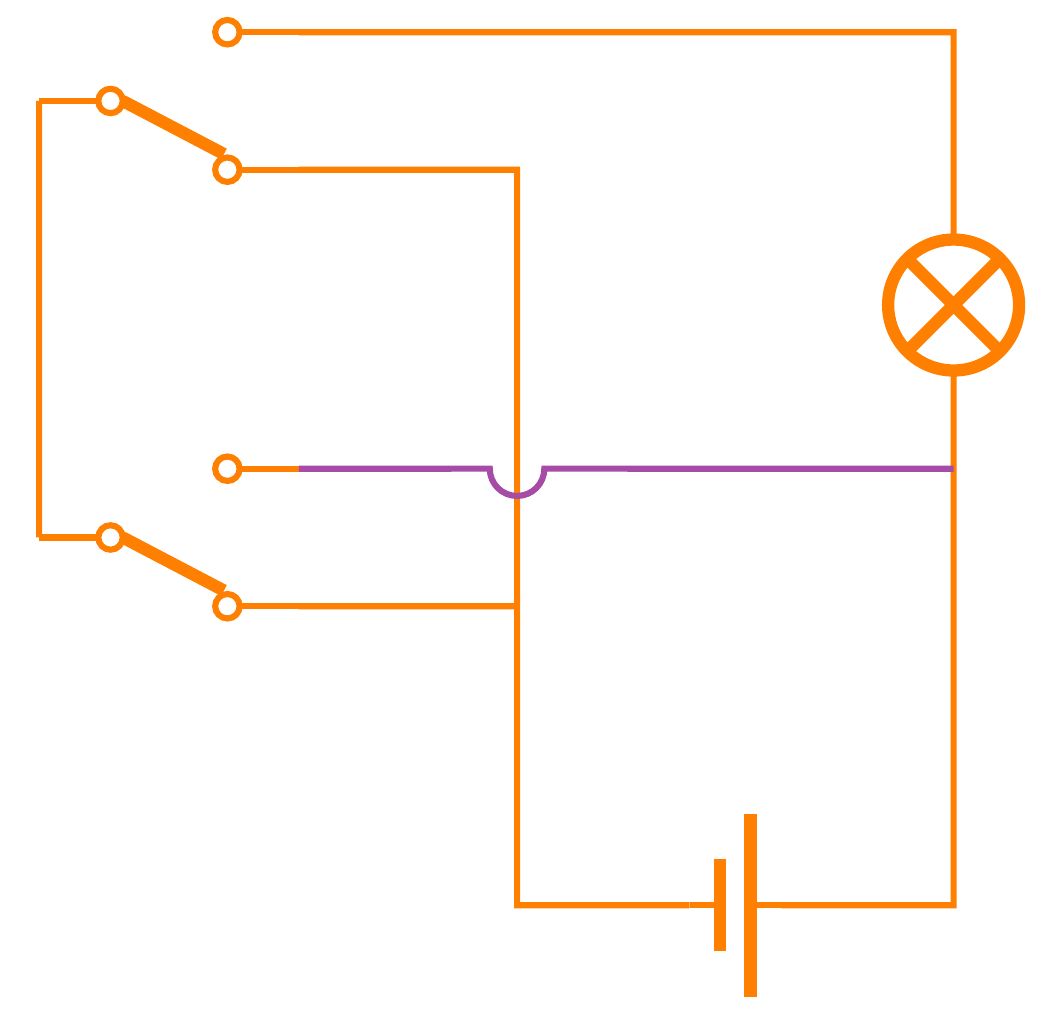
\includegraphics[width=0.50\textwidth]{gambar/Electric_circuit}}
	\caption{Contoh Penggambaran}
	\label{contoh}
\end{figure}	

\noindent
Berikut ini adalah gambar dari source code yang diatas.
\par 

\noindent 
Sementara Tikz menawarkan banyak fitur dan paket untuk membuat diagram dan segala macam gambar lainnya, namun sayangnya tidak ada paket yang bagus untuk tata letak sirkuit listrik. Dengan menggunakan paket circuitikz kita bisa dengan mudah menyelesaikan masalah ini. Ini meluas menyediakan lingkungan baru circuitikz di mana kita dapat dengan mudah menarik sirkuit kita dalam waktu singkat. Sintaksnya sama persis seperti yang ditunjukkan pada pelajaran sebelumnya, jadi kita bisa langsung memulai dengan contoh kode sederhana:
\par

\begin{verbatim}
\ documentclass {article}
\ usepackage {tikz}
\ usepackage {circuitikz}
\ begin {document}
\ begin {figure} [h!]
\ begin {center}
\ begin {circuitikz}
\ draw (0,0)

\end{verbatim}


\noindent 
 ke [V, v = $\$$ U$ \_ $q $\$$] (0,2)$\%$ Sumber tegangan
\par


\noindent 
 ke [pendek] (2,2)
\par


\noindent 
 ke [R = $\$$ R$ \_ $1 $\$$] (2,0)$\%$ Resistornya
\par


\noindent 
 ke [pendek] (0,0);
\par

\begin{verbatim}
\ end {circuitikz}
\ caption {sirkuit pertamaku.}
\ end {center}
\ end {figure}
\ end {document} 

\end{verbatim}

\noindent 
Sirkuit akan ditarik dengan cara yang sama seperti jalur di tikz, tapi kami menentukan opsi khusus untuk elemen:
\par


\noindent 
~ $\setminus$ draw (0,0)
\par


\noindent 
 ke [V, v = $\$$ U$ \_ $q $\$$] (0,2)$\%$ Sumber tegangan 
\par


\noindent 
Mulai dari (0,0) kita akan menggambar sumber tegangan yang menentukan opsi [V, v = UqUq] ke koordinat (0,2), di mana V memilih simbol untuk sumber tegangan dan v = UqUq Menarik panah voltase di sebelahnya. Lalu kita lanjutkan ke resistor:
\par


\noindent 
~ ke [pendek] (2,2)
\par


\noindent 
 ke [R = $\$$ R$ \_ $1 $\$$] (2,0)$\%$ Resistornya 
\par


\noindent 
Pertama kita harus menarik hubung singkat dari (0,2) ke (2,2) dan kemudian letakkan simbol resistor pada jalur dari (2,2) sampai (2,0) perhatikan bahwa kali ini label elemen harus ditentukan secara langsung ( R = R1R1 ) .
\par


\noindent 
Daftar semua elemen yang tersedia untuk rangkaian tersedia dalam manual circuitikz.
\par


\noindent 
Tapi bagaimana kita bisa menambahkan lebih banyak elemen ke sirkuit? Katakanlah kita ingin menambahkan sebuah induktor sejajar dengan Resistor. Cara termudah adalah dengan menambahkan perintah draw baru seperti ini:
\par


\noindent 
~ $\setminus$ begin $ \{ $circuitikz$ \} $
\par


\noindent 
 $\setminus$ draw (0,0)
\par


\noindent 
 ke [V, v = $\$$ U$ \_ $q $\$$] (0,2)$\%$ Sumber tegangan
\par


\noindent 
 ke [pendek] (2,2)
\par


\noindent 
 ke [R = $\$$ R$ \_ $1 $\$$] (2,0)$\%$ Resistornya
\par


\begin{enumerate}
	\item ke [pendek] (0,0);
	\item menarik (2,2)
	\item ke [pendek] (4,2)
	\item ke [L = $\$$ L$ \_ $1 $\$$] (4,0)
	\item ke [pendek] (2,0);
	\item end $ \{ $circuitikz$ \} $
\end{enumerate}



\noindent 
Menambahkan kapasitor di sampingnya, sama sederhananya:
\par


\noindent 
~ $\setminus$ begin $ \{ $circuitikz$ \} $
\par


\noindent 
 $\setminus$ draw (0,0)
\par


\noindent 
 ke [V, v = $\$$ U$ \_ $q $\$$] (0,2)$\%$ Sumber tegangan
\par


\noindent 
 ke [pendek] (2,2)
\par


\noindent 
 ke [R = $\$$ R$ \_ $1 $\$$] (2,0)$\%$ Resistornya
\par


\noindent 
 ke [pendek] (0,0);
\par


\noindent 
 menarik (2,2)
\par


\noindent 
 ke [pendek] (4,2)
\par


\noindent 
 ke [L = $\$$ L$ \_ $1 $\$$] (4,0)
\par


\noindent 
 ke [pendek] (2,0);
\par


\noindent 
 menarik (4,2)
\par


\noindent 
 ke [pendek] (6,2)
\par


\noindent 
 ke [C = $\$$ C$ \_ $1 $\$$] (6,0)
\par


\noindent 
 ke [pendek] (4,0);
\par


\noindent 
 $\setminus$ end $ \{ $circuitikz$ \} $ 
\par


\noindent 
Manual circuitikz memberikan contoh semua simbol dan fungsi dan juga dapat digunakan untuk referensi lebih lanjut.
\par

\subsection{Ringkasan}


\noindent 
Circuitikz menyediakan lingkungan untuk menggambar diagram sirkuit listrik
\par


\noindent 
Sintaksnya mirip dengan sintaks Tikz polos
\par


\noindent 
Daftar semua simbol tersedia dalam manual circutikz
\par


\noindent 
cara menggambar rangkaian listrik sederhana dalam dokumen LaTeX. Untuk melakukan ini kita akan menggunakan paket circuitikz yang berbasis pada paket TikZ. Untuk memulai kami mengisi paket circuitikz.
\par


\noindent 
$\setminus$usepackage$ \{ $circuitikz$ \} $ 
\par


\noindent 
Kami tidak perlu memuat paket TikZ juga karena secara otomatis dimuati dengan circuitikz.Untuk menggambar diagram kita menggunakan lingkungan circuitikz. Kami kemudian mengisi lingkungan dengan satu perintah $\setminus$draw berakhir dalam titik koma.
\par


\noindent 
 $\setminus$begin$ \{ $circuitikz$ \} $ $\setminus$draw <circuitikz code> ; $\setminus$end$ \{ $circuitikz$ \} $ 
\par


\noindent 
Format umum adalah sepasang koordinat yang diikuti oleh sebuah tautan dan kemudian pasangan koordinat berikutnya. Anda kemudian dapat terus menambahkan tautan dan koordinat lebih lanjut seperti rantai. Tautannya bisa berupa garis yang diraih dengan menggunakan dua tanda hubung, atau bisa juga komponen elektrik. Untuk menambahkan komponen pada sebuah garis kita menggunakan kata kunci 'to' diikuti dengan tanda kurung siku yang berisi nama komponen.
\par


\noindent 
Misalnya kita akan mulai dari (0,0) dan menuju ke (0,4) menambahkan baterai masuk. Kita kemudian akan menambahkan ammeter dalam perjalanan menuju (4,4) diikuti oleh garis sederhana ke (4 , 0). Kami akan menyelesaikan rangkaian dengan menambahkan lampu dalam perjalanan pulang (0,0).
\par


\noindent 
 $\setminus$begin$ \{ $circuitikz$ \} $ $\setminus$draw (0,0) to[battery] (0,4) to[ammeter] (4,4) -- (4,0) to[lamp] (0,0) ; $\setminus$end$ \{ $circuitikz$ \} $ 
\par


\noindent 
Inilah diagram yang terlihat seperti dikompilasi.
\par


\noindent 
Sekarang mari kita tambahkan voltmeter yang sejajar dengan lampu. Untuk melakukan ini, kami ingin bercabang dari garis bawah sepanjang jalan, lalu turun ke bawah, masukkan meter, lalu bergabung kembali dengan garis bawah sebelum akhirnya.
\par


\noindent 
 $\setminus$begin$ \{ $circuitikz$ \} $ $\setminus$draw (0,0) to[battery] (0,4) to[ammeter] (4,4) -- (4,0) to[lamp] (0,0) (0.5,0) -- (0.5,-2) to[voltmeter] (3.5,-2) -- (3.5,0) ; $\setminus$end$ \{ $circuitikz$ \} $ 
\par


\noindent 
Jika kita ingin membuat titik di mana garis bergabung ke terminal yang tepat yang diwakili oleh lingkaran, kita bisa menambahkan *-* ke dalam tanda kurung siku di mana kita menambahkan lampu masuk Ini akan menambahkan terminal di koordinat kedua sisi komponen . Oleh karena itu kita perlu memperpendek garis kedua sisi lampu sehingga terminal muncul di garis kita bergabung, dan kemudian kita perlu mengisi kekosongan.
\par


\noindent 
 $\setminus$begin$ \{ $circuitikz$ \} $ $\setminus$draw (0,0) to[battery] (0,4) to[ammeter] (4,4) -- (4,0) -- (3.5,0) to[lamp, *-*] (0.5,0) -- (0,0) (0.5,0) -- (0.5,-2) to[voltmeter] (3.5,-2) -- (3.5,0) ; $\setminus$end$ \{ $circuitikz$ \} $ 
\par


\noindent 
Selanjutnya kita akan menambahkan sebuah kapasitor di antara lampu dan ammeter. Kami tentukan kapasitor dengan modal C.
\par


\noindent 
 $\setminus$begin$ \{ $circuitikz$ \} $ $\setminus$draw (0,0) to[battery] (0,4) to[ammeter] (4,4) to[C] (4,0) -- (3.5,0) to[lamp, *-*] (0.5,0) -- (0,0) (0.5,0) -- (0.5,-2) to[voltmeter] (3.5,-2) -- (3.5,0) ; $\setminus$end$ \{ $circuitikz$ \} $ 
\par


\noindent 
Seringkali kami ingin menambahkan label ke diagram kami untuk memberi lebih banyak informasi kepada pembaca. Untuk dapat memasukkan unit listrik ke label kami, kami perlu menambahkan opsi 'siunitx' ke dalam $\setminus$usepackage .
\par


\noindent 
 $\setminus$usepackage[siunitx]$ \{ $circuitikz$ \} $ 
\par


\noindent 
Kita bisa menambahkan label ke ammeter seperti ini.
\par


\noindent 
 to[ammeter, l=2<$\setminus$ampere>] 
\par


\noindent 
'Saya mengatakan kepada LaTeX bahwa kami menambahkan sebuah label. Perhatikan bahwa kita menempatkan perintah unit dalam kurung kurawal. Karena kita menggunakan unit SI, kita bisa menambahkan awalan SI ke dalam. Kita juga bisa memindahkan label ke bawah simbol dengan menambahkan garis bawah segera setelah 'l'.
\par


\noindent 
 to[ammeter, l$ \_ $=2<$\setminus$milli$\setminus$ampere>] 
\par


\noindent 
Seperti yang kita tampilkan saat ini, kita bisa meletakkan label di sebelah panah di garis dengan mengubah 'l' menjadi 'i'.
\par


\noindent 
 to[ammeter, i$ \_ $=2<$\setminus$milli$\setminus$ampere>] 
\par


\noindent 
Mari tambahkan beberapa label di samping kapasitor dan voltmeter. Dengan kapasitor kita bisa saja memulai label dengan sama dengan mengikuti modal 'C'.
\par


\noindent 
 $\setminus$begin$ \{ $circuitikz$ \} $ $\setminus$draw (0,0) to[battery] (0,4) to[ammeter, i$ \_ $=2<$\setminus$milli$\setminus$ampere>] (4,4) to[C=3<$\setminus$farad>] (4,0) -- (3.5,0) to[lamp, *-*] (0.5,0) -- (0,0) (0.5,0) -- (0.5,-2) to[voltmeter, l=3<$\setminus$kilo$\setminus$volt>] (3.5,-2) -- (3.5,0) ; $\setminus$end$ \{ $circuitikz$ \} $ 
\par


\noindent 
Kita juga bisa mengubah warna komponen seperti ini.
\par


\noindent 
 to[voltmeter, l=3<$\setminus$kilo$\setminus$volt>, color=red] 
\par


\noindent 
Kita dapat mengubah ukuran diagram dengan menambahkan faktor penskalaan sebagai pilihan pada akhir perintah $\setminus$begin .
\par


\noindent 
 $\setminus$begin$ \{ $circuitikz$ \} $[scale=2] $\setminus$draw 
\par


\noindent 
Perhatikan bahwa komponen tetap berukuran sama namun jarak antar segala perubahan.
\par


\noindent 
Mari selesaikan postingan ini dengan melihat pilihan komponen lain yang bisa kita gunakan:
\par


\noindent 
 $\setminus$begin$ \{ $circuitikz$ \} $ $\setminus$draw (0,0) to[R, oo] (2,0) (4,0) to[vR, oo] (6,0) (0,2) to[transmission line, oo] (2,2) (4,2) to[closing switch, oo] (6,2) (0,4) to[european current source, oo] (2,4) (4,4) to[european voltage source, oo] (6,4) (0,6) to[empty diode, oo] (2,6) (4,6) to[full led, oo] (6,6) (0,8) to[generic, oo] (2,8) (4,8) to[sinusoidal voltage source, oo] (6,8) ; $\setminus$end$ \{ $circuitikz$ \} $ 
\par


\noindent 
Contoh ini semua bipoles.
\par


\noindent 
Dari kiri bawah kita miliki; sebuah resistor, resistor variabel, saluran transmisi, saklar penutup, sumber arus eropa, sumber tegangan eropa, dioda kosong, led penuh, bipol generik dan sumber tegangan sinusoidal.
\par


\noindent 
Bipoles bukan satu-satunya jenis komponen yang bisa kita gunakan. Kita juga bisa menambahkan monopoles, tripol, double bipoles, gerbang logika dan amplifier. Namun, kami tidak dapat menggunakan kata kunci 'to' untuk menambahkan ini seperti yang telah kami lakukan sebelumnya, karena keduanya tidak sesuai dengan satu baris saja. Sebagai gantinya kita menggunakan notasi node. Sebagai contoh, ini adalah bagaimana kita akan menampilkan antena:
\par


\noindent 
 (0,0) node[antenna] $ \{ $$ \} $ 
\par


\noindent 
Anda dapat menambahkan teks ke simbol menggunakan kurung kurawal, namun perhatikan bahwa kita masih perlu memasukkan kurung kurawal meskipun kita tidak ingin menggunakannya. Berikut adalah beberapa contoh lagi:
\par


\noindent 
 (4,0) node[pmos] $ \{ $$ \} $ (0,4) node[op amp] $ \{ $$ \} $ (4,4) node[american or port] $ \{ $$ \} $ (0,8) node[transformer] $ \{ $$ \} $ (4,8) node[spdt] $ \{ $$ \} $ 
\par


\noindent 
Untuk kemudian menghubungkannya dengan komponen lain, kita akan menggunakan jangkar simpul yang telah ditentukan. Untuk informasi lebih lanjut tentang semua komponen yang tersedia dan bagaimana Anda menghubungkan komponen menggunakan jangkar simpul, lihat dokumentasinya .
\par


\subsection{Pengantar}


\noindent 
Seperti yang kita pelajari di pelajaran 12, circuitikz adalah alat yang ampuh untuk pembuatan sirkuit. Tapi ada beberapa jebakan di sepanjang jalan. Manual circuitikz memberikan referensi bagus untuk semua komponen yang tersedia, namun tidak memiliki penjelasan mendalam tentang bagaimana menggunakan setiap elemen. Pada dasarnya, ada tiga jenis komponen penting yang tersedia di circuitikz, yaitu monopoles, bipoles dan tripole.Komponen lain yang disebutkan dalam manual dapat digunakan dengan cara yang mirip dengan kelas yang disebutkan dalam tutorial ini.
\par


\noindent 
Garis
\par


\noindent 
Sebelum saya masuk ke berbagai komponen, izinkan saya menunjukkan cara mengubah tampilan garis dasar di circuitikz.Perhatikan contoh berikut ini:
\par


\noindent 
~ $\setminus$ begin $ \{ $figure$ \} $ [h!]
\par


\noindent 
 $\setminus$ begin $ \{ $circuitikz$ \} $
\par


\noindent 
~~ $\setminus$ draw (-1,0) ke [pendek, oo] (1,0);
\par


\noindent 
 $\setminus$ end $ \{ $circuitikz$ \} $
\par


\noindent 
 $\setminus$ end $ \{ $figure$ \} $ 
\par


\noindent 
Seperti yang bisa Anda lihat, sintaksnya sedikit berubah dari pelajaran sebelumnya. Baris pertama hampir sama. Baris pertama akan menarik segmen garis atas dengan konektor terbuka di setiap ujungnya. Konektor dapat dipilih dengan mengubah bagian oo dalam kode.
\par


\noindent 
Jika kita ingin mengganti konektor, pertimbangkan contoh berikut, yang akan menghasilkan output ini:
\par


\noindent 
~ $\setminus$ begin $ \{ $figure$ \} $ [h!]
\par


\noindent 
 $\setminus$ begin $ \{ $circuitikz$ \} $
\par


\noindent 
~~ $\setminus$ draw (-1,0) ke [pendek, * -] (1,0);
\par


\noindent 
 $\setminus$ end $ \{ $circuitikz$ \} $
\par


\noindent 
 $\setminus$ end $ \{ $figure$ \} $ 
\par


\noindent 
Notasi untuk konektor cukup mudah. Anda bisa memilih jenis konektor di setiap ujung garis dengan menggunakan simbol * atau o. Selain itu Anda dapat memilih hanya satu ujung atau kedua ujung garis yang harus memiliki simbol semacam ini misalnya o-, -o atau oo. Jika Anda sama sekali tidak menginginkan konektor, cukup tulis ke [pendek] tanpa simbol tambahan.
\par


\noindent 
Monopoles
\par


\noindent 
Saya akan memulai dengan monopoles, yang merupakan komponen sirkuit yang paling dasar. Kelas ini berisi simbol seperti ground nodes dan antenna. Jadi mari kita lihat lebih dekat contoh yang sebenarnya.
\par


\noindent 
~ $\setminus$ begin $ \{ $figure$ \} $ [h!]
\par


\noindent 
 $\setminus$ begin $ \{ $circuitikz$ \} $
\par


\noindent 
~~ $\setminus$ draw (-1,0) ke [pendek, oo] (1,0);
\par


\noindent 
~~ $\setminus$ draw (0,0) ke [short] node [ground] $ \{ $$ \} $ (0, -1);
\par


\noindent 
 $\setminus$ end $ \{ $circuitikz$ \} $
\par


\noindent 
 $\setminus$ end $ \{ $figure$ \} $ 
\par


\noindent 
Saya mengambil garis dari bagian pertama, namun menambahkan simpul ke tanah. Seperti yang Anda lihat, garis berbeda dalam komponen tidak ditentukan sebagai bipole yang menggunakan operator, tapi sebagai simpul tipe tanah (simpul [ground]). Sangat penting, bahwa setiap simpul memiliki label di tikz. Label ini dapat dibiarkan kosong, namun sintaksnya harus berupa simpul [options] $ \{ $$ \} $. Jika kita memutuskan untuk memberi nama simpul kita, kita bisa menulis teks di antara kawat gigi seperti
\par


\noindent 
~ $\setminus$ begin $ \{ $figure$ \} $ [h!]
\par


\noindent 
 $\setminus$ begin $ \{ $circuitikz$ \} $
\par


\noindent 
~~ $\setminus$ draw (-1,0) ke [pendek, oo] (1,0);
\par


\noindent 
~~ $\setminus$ draw (0,0) ke [short] node [ground] $ \{ $GND$ \} $ (0, -1);
\par


\noindent 
 $\setminus$ end $ \{ $circuitikz$ \} $
\par


\noindent 
 $\setminus$ end $ \{ $figure$ \} $ 
\par


\noindent 
Itu semua ada pada monopoles di circuitikz.
\par


\noindent 
Bipoles
\par


\noindent 
Saya sudah membahas bipoles di pelajaran 12, tapi saya ingin menjelaskan beberapa fitur lanjutan lainnya di sini. Sebagian besar waktu, kita ingin memiliki panah untuk menunjukkan arus atau tegangan di sirkuit kita. Circuitikz menyediakan pilihan yang mudah digunakan untuk menambahkannya ke sirkuit Anda. Contoh di sini pada dasarnya diambil dari manual circuitikz, jadi Anda bisa menemukan beberapa contoh lagi di sana, tapi saya pikir mereka seharusnya tidak hilang dalam tutorial saya, karena ini adalah fitur yang sangat penting.
\par


\noindent 
Panah saat ini
\par


\noindent 
Cara paling dasar untuk menambahkan panah saat ini ke bipole Anda adalah dengan menentukan pilihan i untuk komponen masing-masing. Secara default, arah panah dan posisi label ditentukan oleh circuitikz, namun Anda dapat mengganti pengaturan tersebut untuk meningkatkan keterbacaan.
\par


\noindent 
~ $\setminus$ begin $ \{ $figure$ \} $ [h!]
\par


\noindent 
 $\setminus$ begin $ \{ $circuitikz$ \} $
\par


\noindent 
~~ $\setminus$ draw (0,0) ke [R, i = $\$$ i$ \_ $1 $\$$] (2,0);
\par


\noindent 
 $\setminus$ end $ \{ $circuitikz$ \} $
\par


\noindent 
 $\setminus$ end $ \{ $figure$ \} $ 
\par


\noindent 
Jika Anda ingin mengubah arah panah, Anda bisa menggunakan kode berikut sebagai gantinya. Operator <atau> dapat digunakan untuk menunjukkan arah panah.
\par


\noindent 
~ $\setminus$ begin $ \{ $figure$ \} $ [h!]
\par


\noindent 
 $\setminus$ begin $ \{ $circuitikz$ \} $
\par


\noindent 
~~ $\setminus$ draw (0,0) ke [R, i <= $\$$ i$ \_ $1 $\$$] (2,0);
\par


\noindent 
 $\setminus$ end $ \{ $circuitikz$ \} $
\par


\noindent 
 $\setminus$ end $ \{ $figure$ \} $ 
\par


\noindent 
Selanjutnya kita bisa memanipulasi posisi label i1i1 dengan menggunakan operator $ \string^ $ atau $ \_ $, yang berada di atas dan di bawah garis. Pertama lihat hasilnya untuk operator pertama:
\par


\noindent 
~ $\setminus$ begin $ \{ $figure$ \} $ [h!]
\par


\noindent 
 $\setminus$ begin $ \{ $circuitikz$ \} $
\par


\noindent 
~~ $\setminus$ draw (0,0) ke [R, i $ \string^ $ = $\$$ i$ \_ $1 $\$$] (2,0);
\par


\noindent 
 $\setminus$ end $ \{ $circuitikz$ \} $
\par


\noindent 
 $\setminus$ end $ \{ $figure$ \} $
\par


\noindent 
Sekarang kita ingin menempatkan label di bawah ini:
\par


\noindent 
~ $\setminus$ begin $ \{ $figure$ \} $ [h!]
\par


\noindent 
 $\setminus$ begin $ \{ $circuitikz$ \} $
\par


\noindent 
~~ $\setminus$ draw (0,0) ke [R, i $ \_ $ = $\$$ i$ \_ $1 $\$$] (2,0);
\par


\noindent 
 $\setminus$ end $ \{ $circuitikz$ \} $
\par


\noindent 
 $\setminus$ end $ \{ $figure$ \} $ 
\par


\noindent 
Dua jenis operator dapat dikombinasikan untuk mengubah posisi panah ke sisi kiri atau kanan bipole. Untuk menempatkan panah di sisi kiri, cukup tulis
\par


\noindent 
~ $\setminus$ begin $ \{ $figure$ \} $ [h!]
\par


\noindent 
 $\setminus$ begin $ \{ $circuitikz$ \} $
\par


\noindent 
~~ $\setminus$ draw (0,0) ke [R, i <$ \_ $ = $\$$ i$ \_ $1 $\$$] (2,0);
\par


\noindent 
 $\setminus$ end $ \{ $circuitikz$ \} $
\par


\noindent 
 $\setminus$ end $ \{ $figure$ \} $ 
\par


\noindent 
dan ubah arah untuk menempatkannya di sisi kanan seperti ini
\par


\noindent 
~ $\setminus$ begin $ \{ $figure$ \} $ [h!]
\par


\noindent 
 $\setminus$ begin $ \{ $circuitikz$ \} $
\par


\noindent 
~~ $\setminus$ draw (0,0) ke [R, i $ \_ $> = $\$$ i$ \_ $1 $\$$] (2,0);
\par


\noindent 
 $\setminus$ end $ \{ $circuitikz$ \} $
\par


\noindent 
 $\setminus$ end $ \{ $figure$ \} $ 
\par


\noindent 
Panah voltase
\par


\noindent 
Panah tegangan bisa digunakan dengan cara yang sama seperti panah saat ini, tapi kali ini, gunakan opsi v sebagai gantinya.
\par


\noindent 
~ $\setminus$ begin $ \{ $figure$ \} $ [h!]
\par


\noindent 
 $\setminus$ begin $ \{ $circuitikz$ \} $
\par


\noindent 
~~ $\setminus$ draw (0,0) ke [R, v $ \_ $> = $\$$ v$ \_ $1 $\$$] (2,0);
\par


\noindent 
 $\setminus$ end $ \{ $circuitikz$ \} $
\par


\noindent 
 $\setminus$ end $ \{ $figure$ \} $ 
\par


\noindent 
Seperti yang bisa Anda lihat, operator yang sama berlaku untuk memanipulasi posisi dan arah panah
\par


\noindent 
~ $\setminus$ begin $ \{ $figure$ \} $ [h!]
\par


\noindent 
 $\setminus$ begin $ \{ $circuitikz$ \} $
\par


\noindent 
~~ $\setminus$ draw (0,0) ke [R, v $ \string^ $ <= $\$$ v$ \_ $1 $\$$] (2,0);
\par


\noindent 
 $\setminus$ end $ \{ $circuitikz$ \} $
\par


\noindent 
 $\setminus$ end $ \{ $figure$ \} $ 
\par


\noindent 
Label
\par


\noindent 
Tentu saja mungkin untuk menambahkan label untuk elemen itu sendiri juga. Kami melakukannya dengan menggunakan opsi l kali ini.
\par


\noindent 
~ $\setminus$ begin $ \{ $figure$ \} $ [h!]
\par


\noindent 
 $\setminus$ begin $ \{ $circuitikz$ \} $
\par


\noindent 
~~ $\setminus$ draw (0,0) ke [R, l $ \string^ $ = $\$$ R$ \_ $1 $\$$] (2,0);
\par


\noindent 
 $\setminus$ end $ \{ $circuitikz$ \} $
\par


\noindent 
 $\setminus$ end $ \{ $figure$ \} $ 
\par


\noindent 
Sebaiknya kita menempatkan label di bawah elemen juga, sekali lagi menggunakan operator $ \_ $:
\par


\noindent 
~ $\setminus$ begin $ \{ $figure$ \} $ [h!]
\par


\noindent 
 $\setminus$ begin $ \{ $circuitikz$ \} $
\par


\noindent 
~~ $\setminus$ draw (0,0) ke [R, l $ \_ $ = $\$$ R$ \_ $1 $\$$] (2,0);
\par


\noindent 
 $\setminus$ end $ \{ $circuitikz$ \} $
\par


\noindent 
 $\setminus$ end $ \{ $figure$ \} $ 
\par


\noindent 
Tripoles
\par


\noindent 
Kelompok komponen yang terakhir namun tak kalah pentingnya adalah tripol. Kelompok tripoles yang paling penting tentu saja adalah semua jenis transistor. Anda bisa menemukan keseluruhan daftar contoh untuk transistor beserta yang ini di manual circuitikz, tapi saya jelaskan bagaimana penggunaannya berbeda dari bipoles.
\par


\noindent 
~ $\setminus$ begin $ \{ $figure$ \} $ [h!]
\par


\noindent 
 $\setminus$ begin $ \{ $circuitikz$ \} $
\par


\noindent 
~~ $\setminus$ draw (0,0) node [npn] (npn1) $ \{ $$ \} $
\par


\noindent 
~~ (npn1.base) node [anchor = east] $ \{ $B$ \} $
\par


\noindent 
~~ (npn1.collector) node [anchor = south] $ \{ $C$ \} $
\par


\noindent 
~~ (npn1.emitter) node [anchor = north] $ \{ $E$ \} $;
\par


\noindent 
 $\setminus$ end $ \{ $circuitikz$ \} $
\par


\noindent 
 $\setminus$ end $ \{ $figure$ \} $ 
\par


\noindent 
Tripol adalah simpul dalam circuitikz seperti monopoles, tapi Anda harus menempatkan beberapa jangkar ke masing-masing konektor tripol. Pertama, Anda menentukan nama untuk simpul dalam tanda kurung. Dalam hal ini saya telah memilih nama npn1. Nama ini akan digunakan untuk referensi ke transistor kita nanti. Setelah itu, ketiga jangkar tersebut harus di atur seperti yang terlihat di atas.
\par


\noindent 
Kita sekarang bisa merujuk ke node dan melampirkan beberapa elemen lain ke transistor.
\par


\noindent 
~ $\setminus$ begin $ \{ $figure$ \} $ [h!]
\par


\noindent 
 $\setminus$ begin $ \{ $circuitikz$ \} $
\par


\noindent 
~~ $\setminus$ draw (0,0) node [npn] (npn1) $ \{ $$ \} $
\par


\noindent 
~~ (npn1.base) node [anchor = east] $ \{ $B$ \} $
\par


\noindent 
~~ (npn1.collector) node [anchor = south, xshift = 0.5cm] $ \{ $C$ \} $
\par


\noindent 
~~ (npn1.emitter) node [anchor = north] $ \{ $E$ \} $;
\par


\noindent 
~~ $\setminus$ draw (npn1.collector) ke [R] ++ (0,2);
\par


\noindent 
 $\setminus$ end $ \{ $circuitikz$ \} $
\par


\noindent 
 $\setminus$ end $ \{ $figure$ \} $ 
\par


\noindent 
Perhatikan bahwa saya menambahkan opsi xshift ke nodus, untuk mencegah agar label tidak tumpang tindih dengan elemen baru.Saya harap Anda menikmati penjelasan saya dan yang Anda temukan dengan menggunakan circuitikz jauh lebih membingungkan dari sekarang.
\par


\noindent 
Ringkasan
\par


\noindent 
Ada tiga komponen utama komponen dalam sirkuitikz
\par


\noindent 
Semua kelas lainnya bisa digunakan dengan cara yang mirip dengan kelas utama tersebut
\par


\noindent 
Contoh penggunaan disediakan dalam manual circuitikz
\par


\chapter{Source Code Hightlighting in Latex using the Listing Package (Listing)}
\sloppy
\section{Daftar Sumber Kode LaTeX / Source}

\begin{figure}[ht]
	\centerline{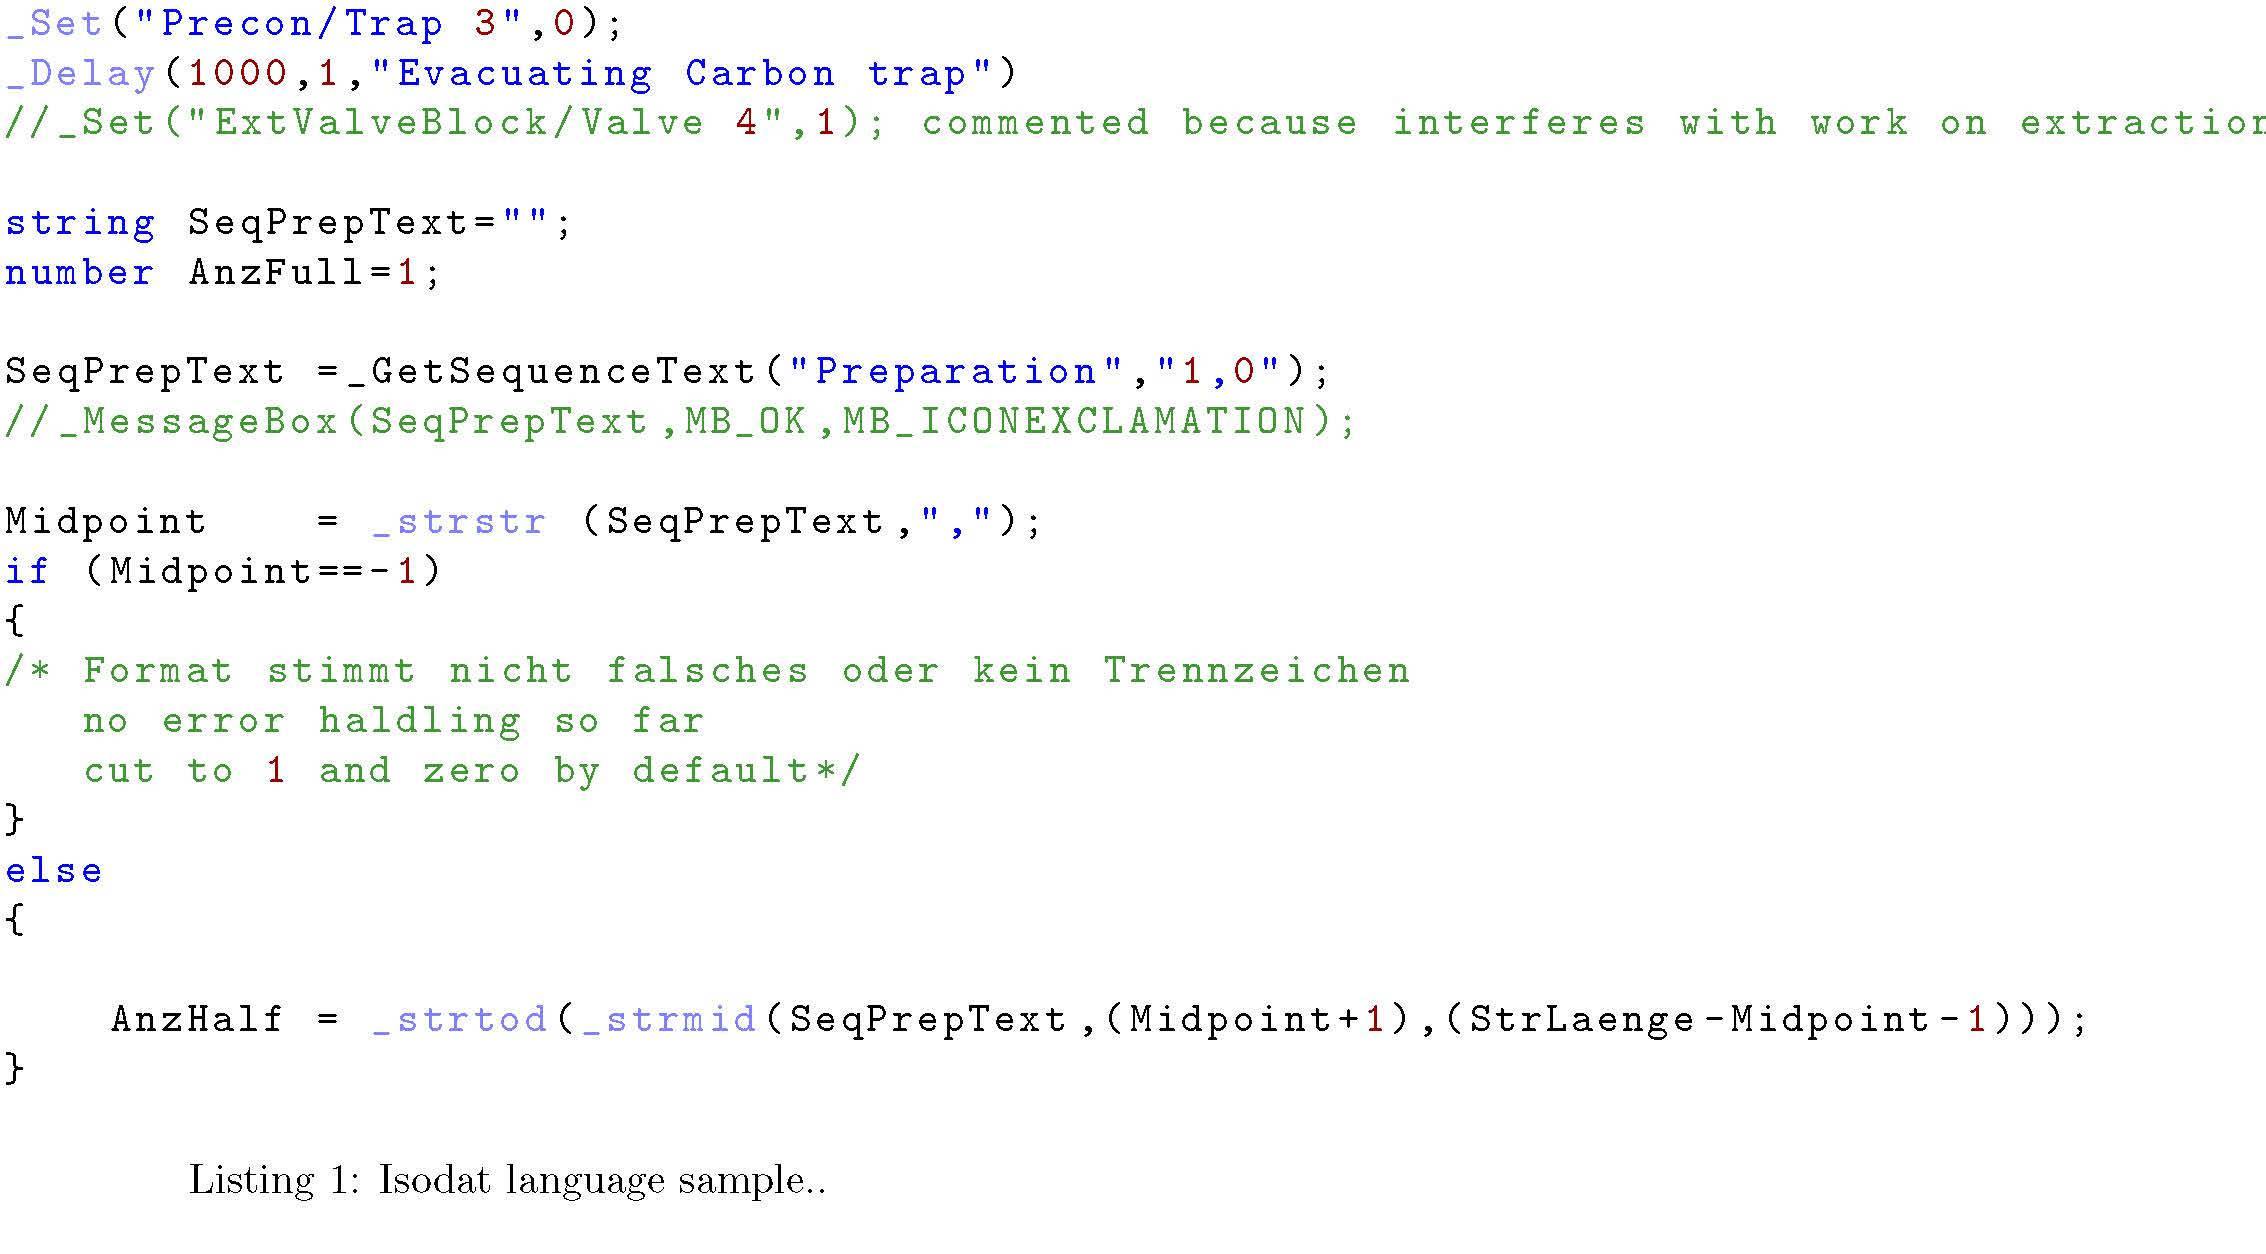
\includegraphics[width=0.50\textwidth]{gambar/contoh1}}
	\caption{Contoh Source code}
	\label{contoh}
\end{figure}

Menggunakan paket daftar \par

Dengan menggunakan daftar paket Anda dapat menambahkan teks yang tidak diformat seperti yang akan Anda lakukan dengan $\textbackslash$begin $ \{ $ verbatim $ \} $ namun tujuan utamanya adalah memasukkan kode sumber dari bahasa pemrograman apa pun ke dalam dokumen Anda. Jika Anda ingin memasukkan pseudocode atau algoritma, Anda mungkin menemukan Algoritma dan Pseudocode berguna juga.\par

Untuk menggunakan paket tersebut, Anda memerlukan:\par

$\textbackslash$ usepackage $ \{ $ listings $ \} $\par

Paket daftar mendukung penyorotan semua bahasa yang paling umum dan sangat mudah disesuaikan. Jika Anda hanya ingin menulis kode dalam dokumen Anda, paket tersebut menyediakan lingkungan lstlisting :\par

$\textbackslash$ begin $ \{ $ lstlisting $ \} $\par

 Letakkan kode anda disini\par

 $\textbackslash$ end $ \{ $ lstlisting $ \} $\par

Kemungkinan lain, itu sangat berguna jika Anda membuat program pada beberapa file dan Anda masih mengeditnya, adalah dengan mengimpor kode dari sumbernya sendiri. Dengan cara ini, jika Anda memodifikasi sumbernya, Anda hanya perlu mengkompilasi ulang kode LaTeX dan dokumen Anda akan diperbarui. Perintahnya adalah:\par

$\textbackslash$ lstinputlisting $ \{ $ source $ \_ $ filename.py $ \} $\par

dalam contoh ada sumber Python, tapi tidak masalah: Anda bisa memasukkan file apapun tapi Anda harus menulis nama file lengkap. Ini akan dianggap teks biasa dan akan disorot sesuai setting Anda, itu berarti tidak mengenali bahasa pemrograman dengan sendirinya. Anda bisa menentukan bahasa sementara menyertakan file dengan perintah berikut:\par

$\textbackslash$ lstinputlisting [language = Python] $ \{ $ source $ \_ $ filename.py $ \} $\par

Anda juga bisa menentukan ruang lingkup untuk file tersebut.\par

$\textbackslash$ lstinputlisting [bahasa = Python, firstline = 37, lastline = 45] $ \{ $ source $ \_ $ filename.py $ \} $\par

Ini sangat berguna jika Anda yakin file tersebut tidak akan berubah (setidaknya sebelum baris yang ditentukan). Anda juga dapat menghilangkan parameter firstline atau lastline : itu berarti semuanya sesuai atau dimulai dari titik ini .\par

Ini adalah contoh dasar untuk beberapa kode Pascal:\par

 $\textbackslash$ documentclass $ \{ $ article $ \} $\par

 $\textbackslash$ usepackage $ \{ $ listings $ \} $ $\%$ Sertakan daftar-paket\par

 $\textbackslash$ begin $ \{ $ document $ \} $\par

 $\textbackslash$ lstset $ \{ $ language = Pascal $ \} $ $\%$ Atur bahasa Anda (Anda dapat mengubah bahasa untuk setiap blok kode secara opsional)\par

 $\textbackslash$ begin $ \{ $ lstlisting $ \} $ [frame = single] $\%$ Mulai blok kode Anda\par

 untuk i: = maxint to 0 do\par

 mulai\par

 $ \{ $ do nothing $ \} $\par

 akhir;\par

 Tulislah ('Case insensitive');\par

 Tulis ('kata kunci Pascal'.);\par

 $\textbackslash$ end $ \{ $ lstlisting $ \} $\par

 $\textbackslash$ end $ \{ $ document $ \} $\par

Bahasa yang didukung \par

Ini mendukung bahasa pemrograman berikut:\par

ABAP 2,4 , ACSL, Ada 4 , Algol 4 , Ant, Assembler 2,4 , Awk 4 , bash, Dasar 2,4 , C $\#$ 5 , C ++ 4 , C 4 , Caml 4 , Clean, Cobol 4 , Comal, csh , Delphi, Eiffel, Elan, erlang, Euforia, Fortran 4 , GCL, Gnuplot, Haskell, HTML, IDL 4 , informasikan, Java 4 , JVMIS, ksh, Lisp 4 , Logo, Lua 2 , buat 4 , Mathematica 1,4 , Matlab, Mercury, MetaPost, Miranda, Mizar, ML, Modelica 3 , Modula-2, MuPAD, NASTRAN, Oberon-2, Tujuan C 5 , OCL 4 , Octave, Oz, Pascal 4 , Perl, PHP, PL / I, Plasm , POV, Prolog, Promela, Python, R, Reduce, Rexx, RSL, Ruby, S 4 , SAS, Scilab, sh, SHELXL, Simula 4 , SQL, tcl 4 , TeX 4 , VBScript, Verilog, VHDL 4 , VRML 4 , XML, XSLT.\par

Bagi beberapa dari mereka, beberapa dialek didukung. Untuk informasi lebih lanjut, lihat dokumentasi yang disertakan dengan paket, harus berada dalam distribusi Anda dengan daftar nama - *. Dvi .\par

Catatan\par

Ini mendukung kode Mathematica hanya jika Anda mengetik dalam format teks biasa. Anda tidak dapat menyertakan file * .NB $\textbackslash$lstinputlisting $ \{ $ ... $ \} $ seperti yang Anda bisa dengan bahasa pemrograman lainnya, namun Mathematica dapat mengekspornya ke sumber LaTeX yang berformat cantik.\par

Spesifikasi dialek adalah wajib untuk bahasa-bahasa ini (misalnya language= $ \{ $ [x86masm]Assembler $ \} $ ).\par

Modelica didukung melalui paket dtsyntax yang tersedia.\par

Untuk bahasa ini, beberapa dialek didukung. C, misalnya, memiliki ANSI, Handel, Objective dan Sharp. Lihat hal. 12 dari manual daftar untuk ikhtisar.\par

Ditetapkan sebagai dialek bahasa lain\par

Pengaturan \par

Anda dapat memodifikasi beberapa parameter yang akan mempengaruhi bagaimana kode ditampilkan. Anda dapat menempatkan kode berikut di manapun dalam dokumen (tidak masalah apakah sebelum atau sesudah $\textbackslash$begin $ \{ $ document $ \} $ ), ubahlah sesuai kebutuhan Anda. Maknanya dijelaskan di samping garis mana saja.\par
\begin{verbatim}
 \ usepackage { listings }
\ usepackage { color }
\ definecolor { mygreen } { rgb } { 0,0.6,0 }
\ definecolor { mygray } { rgb } { 0.5.0.5.0.5 }
\ definecolor { mymauve } { rgb } { 0.58,0,0.82 }
\ lstset { %

\end{verbatim}


~~ backgroundcolor = $\textbackslash$ color $ \{ $ white~$ \} $~, $\%$ pilih warna latar belakang;  Anda harus menambahkan $\textbackslash$ usepackage $ \{ $color$ \} $ or $\textbackslash$ usepackage $ \{ $xcolor$ \} $;  harus datang sebagai argumen terakhir\par

~~ basicstyle = $\textbackslash$ footnotesize , $\%$ ukuran font yang digunakan untuk kode\par

~~ breakatwhitespace = false, $\%$ set jika jeda otomatis seharusnya hanya terjadi di spasi\par

~~ breaklines = true, $\%$ set baris otomatis melanggar\par

~~ captionpos = b, $\%$ set caption-posisi ke bawah\par

~~ commentstyle = $\textbackslash$ color $ \{ $ mygreen $ \} $ , $\%$ style komentar\par

~~ deletekeywords = $ \{ $ ... $ \} $ , $\%$ jika Anda ingin menghapus kata kunci dari bahasa yang diberikan\par

~~ escapeinside = $ \{ $ $\textbackslash$$\%$ * $ \} $ $ \{ $ *) $ \} $ , $\%$ jika Anda ingin menambahkan LaTeX dalam kode Anda\par

~~ extendedchars = true, $\%$ memungkinkan Anda menggunakan karakter non-ASCII;~ untuk pengkodean 8-bit saja, tidak bekerja dengan UTF-8\par

~~ frame = single, $\%$ menambahkan bingkai di sekitar kode\par

~~ keepspaces = true, $\%$ menyimpan spasi di teks, berguna untuk menjaga indentasi kode (mungkin membutuhkan kolom = fleksibel)\par

~~ keywordstyle = $\textbackslash$ color $ \{ $ blue $ \} $ , $\%$ gaya kata kunci\par

~~ bahasa = Octave, $\%$ bahasa kode\par

~~ morekeywords = $ \{ $ *, ... $ \} $ , $\%$ jika Anda ingin menambahkan lebih banyak kata kunci ke himpunan\par

~~ nomor = kiri, $\%$ di mana untuk menempatkan nomor baris;~ nilai yang mungkin adalah (none, left, right)\par

~~ numberep = 5pt, $\%$ seberapa jauh garis-angka dari kode\par

~~ numbertyle = $\textbackslash$ tiny $\textbackslash$ color $ \{ $ mygray $ \} $ , $\%$ style yang digunakan untuk line-numbers\par

~~ rulecolor = $\textbackslash$ color $ \{ $ black $ \} $ , $\%$ jika tidak disetel, warna bingkai dapat berubah pada garis-jeda dalam teks tidak-hitam (misalnya komentar (hijau di sini))\par

~~ showpaces = false, $\%$ show spaces dimana-mana menambahkan garis bawah tertentu;~ itu menimpa 'showstringspaces'\par

~~ showstringspaces = false, $\%$ menggarisbawahi ruang dalam string saja\par

~~ showtabs = false, $\%$ tampilkan tab dalam string yang menambahkan garis bawah tertentu\par

~~~stepnumber = 2, $\%$ langkah antara dua line-numbers.  Jika 1, setiap baris akan diberi nomor\par

~~ stringstyle = $\textbackslash$ color $ \{ $ mymauve $ \} $ , $\%$ string literal style\par

~~ tabsize = 2, $\%$ set tabsize default menjadi 2 spasi\par

~~ title = $\textbackslash$ lstname $\%$ tampilkan nama file yang disertakan dengan $\textbackslash$ lstinputlisting;~ juga mencoba judul dan bukan judul\par

 $ \} $\par

Escapeinside\par

Garis pelarian membutuhkan penjelasan. Pilihan escapeinside= $ \{ $ A $ \} $$ \{ $ B $ \} $ akan menentukan pembatas untuk lolos ke kode LaTeX, yaitu semua kode antara string "A" dan "B" akan diuraikan sebagai LaTeX dari daftar gaya saat ini. Pada contoh di atas, komentar untuk Octave dimulai dengan $\%$ , dan akan dicetak dalam dokumen kecuali jika dimulai dengan $\%$* , dalam hal ini mereka dibaca sebagai LaTeX (dengan semua perintah LaTeX terpenuhi) sampai ditutup dengan yang lain *) . Jika Anda menambahkan paragraf di atas, berikut ini dapat digunakan untuk mengubah pengaturan dalam kode:\par

$\textbackslash$ lstset $ \{ $ language = C, caption = $ \{ $ Teks Keterangan Deskriptif $ \} $ , label = DeskriptifLabel $ \} $\par

Ada lebih banyak pilihan, periksa dokumentasi resmi.\par

Definisi gaya \par

Paket ini memungkinkan Anda menentukan gaya, yaitu profil yang menentukan satu set pengaturan.\par

Contoh\par

\begin{enumerate}
	\item lstdefinestyle  customc 
	\item belowcaptionskip = 1 \ baselineskip ,
	\item	breaklines = true,
	\item	frame = L,
	\item	xleftmargin = \ parindent ,
	\item	bahasa = C,
	\item	showstringspaces = false,
	\item	basicstyle = \ footnotesize \ ttfamily ,
	\item	keywordstyle = \ bfseries \ color  green! 40! black  ,
	\item	commentstyle = \ itshape \ color  ungu! 40! hitam  ,
	\item	identifierstyle = \ color  blue  ,
	\item	stringstyle = \ color  orange  ,
	 \item   lstdefinestyle  customasm 
	\item	belowcaptionskip = 1 \ baselineskip ,
	\item	frame = L,
	\item	xleftmargin = \ parindent ,
	\item	bahasa = [x86masm] Assembler,
	\item	basicstyle = \ footnotesize \ ttfamily ,
	\item	commentstyle = \ itshape \ color  ungu! 40! hitam  ,
	 \item   lstset  escapechar = @, style = customc 
\end{enumerate}



Dalam contoh kita, kita hanya menetapkan dua pilihan secara global: gaya default dan karakter escape. Pemakaian:\par

 $\setminus$ begin $ \{ $ lstlisting $ \} $\par

 $\#$include <stdio.h>\par

 $\#$define N 10\par

 / * Blokir\par

 * komentar * /\par

 int main ()\par

 $ \{ $\par

~~~~ int i ;\par

~~~~ // Baris komentar\par

~~~~ menempatkan ( "Halo dunia!" );\par

~~~ \par

~~~~ untuk ( i = 0 ; i < N ; i ++ )\par

~~~~ $ \{ $\par

~~~~~~~~ menempatkan ( "LaTeX juga bagus untuk pemrogram!" );\par

~~~~ $ \} $\par

~~~~ kembali 0 ;\par

 $ \} $\par

 $\textbackslash$ end $ \{ $ lstlisting $ \} $\par

 $\textbackslash$ lstinputlisting [ caption = Scheduler ,~style = customc ] $ \{ $ halo .  c $ \} $\par

Mengotomatiskan file inclusion \par

Jika Anda memiliki banyak file sumber yang ingin Anda sertakan, Anda mungkin mendapati diri Anda melakukan hal yang sama berulang-ulang. Di sinilah makro menunjukkan kekuatan sesungguhnya mereka.\par

 $\textbackslash$ newcommand $ \{ $ $\textbackslash$ includecode $ \} $ [2] [c] $ \{ $ $\textbackslash$ lstinputlisting [caption = $\#$ 2, escapechar =, style = custom $\#$ 1] $ \{ $ $\#$ 2 $ \} $ <! ----> $ \} $\par

 $\%$ ...\par

 $\textbackslash$ includecode $ \{ $ sched.c $ \} $\par

 $\textbackslash$ includecode [asm] $ \{ $ sched.s $ \} $\par

 $\%$ ...\par

 $\textbackslash$ lstlistoflistings\par

Dalam contoh ini, kita membuat satu perintah untuk memudahkan penyertaan kode sumber. Kami menetapkan gaya default menjadi customc . Semua daftar akan memiliki nama mereka sebagai caption: kita tidak perlu menuliskan nama file dua kali terima kasih kepada makro. Akhirnya kami daftar semua daftar dengan perintah ini dari daftar paket.\par

Lihat Makro untuk lebih jelasnya.\par

Encoding issue \par

Secara default, daftar tidak mendukung pengkodean multi-byte untuk kode sumber. Pilihan extendedchar hanya bekerja untuk pengkodean 8-bit seperti latin1.\par

Untuk menangani UTF-8, Anda harus memberi tahu cantuman bagaimana menafsirkan karakter khusus dengan menentukannya seperti itu\par

 $\textbackslash$ lstset $ \{ $ melek huruf =\par

~~ $ \{ $$ \{ $ $ \} $ $ \} $ $ \{ $$ \{ $ $\textbackslash$ ' $ \} $$ \} $ 1 $ \{ $ í $ \} $ $ \{ $$ \{ $ $\textbackslash$' i $ \} $$ \} $ 1 $ \{ $ ó $ \} $ $ \{ $$ \{ $ $\textbackslash$ ' o $ \} $$ \} $ 1 $ \{ $ ú $ \} $ $ \{ $$ \{ $ $\textbackslash$ ' u $ \} $$ \} $ 1\par

~~ $ \{ $$ \{ $ $ \} $$ \} $ $ \{ $$ \{ $ $\textbackslash$ ' A $ \} $$ \} $ 1 $ \{ $ É $ \} $ $ \{ $$ \{ $ $\textbackslash$' E $ \} $$ \} $ 1 $ \{ $ Í $ \} $ $ \{ $$ \{ $ $\textbackslash$ ' I $ \} $$ \} $ 1 $ \{ $ Ó $ \} $ $ \{ $$ \{ $ $\textbackslash$' O $ \} $$ \} $ 1 $ \{ $ Ú $ \} $ $ \{ $$ \{ $ $\textbackslash$ ' U $ \} $$ \} $ 1\par

~~ $ \{ $ à $ \} $ $ \{ $$ \{ $ $\textbackslash$ ` a $ \} $$ \} $ 1 $ \{ $ è $ \} $ $ \{ $$ \{ $ $\textbackslash$` e $ \} $$ \} $ 1 $ \{ $ ì $ \} $ $ \{ $$ \{ $ $\textbackslash$ ` i $ \} $$ \} $ 1 $ \{ $ ò $ \} $ $ \{ $$ \{ $ $\textbackslash$` o $ \} $$ \} $ 1 $ \{ $ ù $ \} $ $ \{ $$ \{ $ $\textbackslash$ ` u $ \} $$ \} $ 1\par

~~ $ \{ $$ \{ $ $ \} $$ \} $ $ \{ $$ \{ $ $\textbackslash$ $\textbackslash$ $ \} $$ \} $ 1 $ \{ $ È $ \} $ $ \{ $$ \{ $ $\textbackslash$ ' I $ \} $$ \} $ 1 $ \{ $ Ò $ \} $ $ \{ $$ \{ $ $\textbackslash$ ` O $ \} $$ \} $ 1 $ \{ $ Ù $ \} $ $ \{ $$ \{ $ $\textbackslash$ ` U $ \} $$ \} $ 1\par

~~ $ \{ $$ \{ $ $ \} $ $ \} $ $ \{ $$ \{ $ $\textbackslash$ " e $ \} $$ \} $ 1 $ \{ $ ò $ \} $ $ \{ $$ \{ $ $\textbackslash$" i $ \} $$ \} $ 1 $ \{ $ ö $ \} $ $ \{ $$ \{ $ $\textbackslash$ " o $ \} $$ \} $ 1 $ \{ $ ü $ \} $ $ \{ $$ \{ $ $\textbackslash$ " u $ \} $$ \} $ 1\par

~~ $ \{ $ $ \} $ $ \{ $$ \{ $ $\textbackslash$ " A $ \} $$ \} $ 1 $ \{ $ Ë $ \} $ $ \{ $$ \{ $ $\textbackslash$" E $ \} $$ \} $ 1 $ \{ $ Ï $ \} $ $ \{ $$ \{ $ $\textbackslash$ " I $ \} $$ \} $ 1 $ \{ $ Ö $ \} $ $ \{ $$ \{ $ $\textbackslash$" O $ \} $$ \} $ 1 $ \{ $ Ü $ \} $ $ \{ $$ \{ $ $\textbackslash$ " U $ \} $$ \} $ 1\par

~~ $ \{ $ $ \} $ $ \{ $$ \{ $ $\textbackslash$ $ \string^ $ a $ \} $$ \} $ 1 $ \{ $ ê $ \} $ $ \{ $$ \{ $ $\textbackslash$ $ \string^ $ e $ \} $$ \} $ 1 $ \{ $ î $ \} $ $ \{ $$ \{ $ $\textbackslash$ $ \string^ $ i $ \} $$ \} $ 1 $ \{ $ ô $ \} $ $ \{ $$ \{ $ $\textbackslash$ $ \string^ $ o $ \} $$ \} $ 1 $ \{ $ û $ \} $ $ \{ $$ \{ $ $\textbackslash$ $ \string^ $ u $ \} $$ \} $ 1\par

~~ $ \{ $$ \{ $ $ \} $$ \} $ $ \{ $$ \{ $ $ \string^ $ $ \} $$ \} $ $ \{ $$ \{ $ $ \} $$ \} $$ \} $ $ \{ $$ \{ $ $\textbackslash$ $\textbackslash$ $ \} $$ \} $ $ \{ $$ \{ $$ \} $$ \} $$ \} $ $ \{ $$ \{ $ $\textbackslash$ $\textbackslash$ $ \} $$ \} $ $ \{ $$ \{ $ $ \} $ $\textbackslash$ $ \string^ $ I $ \} $$ \} $ 1 $ \{ $ Ô $ \} $ $ \{ $$ \{ $ $\textbackslash$ $ \string^ $ O $ \} $$ \} $ 1 $ \{ $ Û $ \} $ $ \{ $$ \{ $ $\textbackslash$ $ \string^ $ U $ \} $$ \} $ 1\par

~~ $ \{ $ $ \} $ $ \{ $$ \{ $ $\textbackslash$ oe $ \} $$ \} $ 1 $ \{ $ Œ $ \} $ $ \{ $$ \{ $ $\textbackslash$ OE $ \} $$ \} $ 1 $ \{ $ æ $ \} $ $ \{ $$ \{ $ $\textbackslash$ ae $ \} $$ \} $ 1 $ \{ $ Æ $ \} $ $ \{ $$ \{ $ $\textbackslash$ AE $ \} $$ \} $ 1 $ \{ $ ß $ \} $ $ \{ $$ \{ $ $\textbackslash$ ss $ \} $$ \} $ 1\par

~~ $ \{ $ ű $ \} $ $ \{ $$ \{ $ $\textbackslash$ H $ \{ $ u $ \} $$ \} $$ \} $ 1 $ \{ $ Ű $ \} $ $ \{ $$ \{ $ $\textbackslash$ H $ \{ $ U $ \} $$ \} $$ \} $ 1 $ \{ $ ő $ \} $ $ \{ $$ \{ $ $\textbackslash$ H $ \{ $ o $ \} $$ \} $$ \} $ 1 $ \{ $ Ő $ \} $ $ \{ $$ \{ $ $\textbackslash$ H $ \{ $ O $ \} $$ \} $ $ \} $ 1\par

~~ $ \{ $ ç $ \} $ $ \{ $$ \{ $ c $ \} $$ \} $ 1 $ \{ $ Ç $ \} $ $ \{ $$ \{ $ c $ \} $$ \} $ 1 $ \{ $ ø $ \} $ $ \{ $$ \{ $ $\textbackslash$ o $ \} $$ \} $ 1 $ \{ $ å $ \} $ $ \{ $$ \{ $ $\textbackslash$ $\textbackslash$ $ \} $$ \} $ 1 $ \{ $ Å $ \} $ $ \{ $$ \{ $ $\textbackslash$ r A $ \} $$ \} $ 1\par

~~ $ \{ $ € $ \} $ $ \{ $$ \{ $ $\textbackslash$ euro $ \} $$ \} $ 1 $ \{ $ £ $ \} $ $ \{ $$ \{ $ $\textbackslash$ pound $ \} $$ \} $ 1 $ \{ $ « $ \} $ $ \{ $$ \{ $ $\textbackslash$ guillemotleft $ \} $$ \} $ 1\par

~~ $ \{ $ $ \} $$ \} $ $ \{ $$ \{ $ $\textbackslash$ Guillemotright $ \} $$ \} $ 1 $ \{ $ ñ $ \} $ $ \{ $$ \{ $ $\textbackslash$ $ \sim $ n $ \} $$ \} $ 1 $ \{ $ Ñ $ \} $ $ \{ $$ \{ $ $\textbackslash$ $ \sim $ N $ \} $$ \} $ 1 $ \{ $ ¿ $ \} $ $ \{ $$ \{ $ ? ` $ \} $$ \} $ 1\par

 $ \} $\par

Tabel di atas akan mencakup sebagian besar karakter dalam bahasa latin. Untuk penjelasan lebih rinci tentang penggunaan bagian cek pilihan literate 6.4 di Dokumentasi Listing .\par

Kemungkinan lain adalah mengganti $\textbackslash$usepackage $ \{ $ listings $ \} $ (dalam basa-basi) dengan $\textbackslash$usepackage $ \{ $ listingsutf8 $ \} $ , tapi ini hanya akan bekerja untuk $\textbackslash$lstinputlisting $ \{ $ ... $ \} $ .\par

Menyesuaikan caption \par

Anda dapat memiliki caption mewah (atau judul) untuk cantuman Anda menggunakan paket teks . Berikut adalah contoh untuk daftar .\par

 $\textbackslash$ usepackage $ \{ $ caption $ \} $\par

 $\textbackslash$ usepackage $ \{ $ listings $ \} $\par

 $\textbackslash$ DeclareCaptionFont $ \{ $ white $ \} $ $ \{ $ $\textbackslash$ color $ \{ $ white $ \} $ $ \} $\par

 $\textbackslash$ DeclareCaptionFormat $ \{ $ listing $ \} $ $ \{ $\par

~~ $\textbackslash$ colorbox [cmyk] $ \{ $ 0.43, 0.35, 0.35.0.01 $ \} $ $ \{ $\par

~~~~ $\textbackslash$ parbox $ \{ $ $\textbackslash$ textwidth $ \} $ $ \{ $ $\textbackslash$ hspace $ \{ $ 15pt $ \} $ $\#$ 1 $\#$ 2 $\#$ 3 $ \} $\par

~~ $ \} $\par

 $ \} $\par

 $\textbackslash$ capionsetup [lstlisting] $ \{ $ format = daftar, labelfont = putih, textfont = putih, singlelinecheck = false, margin = 0pt, font = $ \{ $ bf, footnotesize $ \} $ $ \} $\par

 $\%$ ...\par

 $\textbackslash$ lstinputlisting [caption = My caption] $ \{ $ sourcefile.lang $ \} $\par

Paket yang dicetak \par

dicetak adalah alternatif untuk daftar yang telah menjadi populer. Menggunakan Python eksternal perpustakaan Pygments untuk menyoroti kode, yang pada November 2014 menawarkan lebih dari 300 bahasa dan format teks yang didukung.\par

Karena paket bergantung pada kode Python eksternal, penyiapan memerlukan beberapa langkah lebih banyak daripada paket LaTeX biasa, jadi mohon lihat repo GitHub dan manualnya .\par

Catatan\par

Ini mendukung kode Mathematica hanya jika Anda mengetik dalam format teks biasa. Anda tidak dapat menyertakan file * .NB $\textbackslash$lstinputlisting $ \{ $ ... $ \} $ seperti yang Anda bisa dengan bahasa pemrograman lainnya, namun Mathematica dapat mengekspornya ke sumber LaTeX yang berformat cantik.\par

Spesifikasi dialek adalah wajib untuk bahasa-bahasa ini (misalnya language= $ \{ $ [x86masm]Assembler $ \} $ ).\par

Modelica didukung melalui paket dtsyntax yang tersedia.\par

Untuk bahasa ini, beberapa dialek didukung. C, misalnya, memiliki ANSI, Handel, Objective dan Sharp. Lihat hal. 12 dari manual daftar untuk ikhtisar.\par

Ditetapkan sebagai dialek bahasa lain\par

Pengaturan \par

Anda dapat memodifikasi beberapa parameter yang akan mempengaruhi bagaimana kode ditampilkan. Anda dapat menempatkan kode berikut di manapun dalam dokumen (tidak masalah apakah sebelum atau sesudah $\textbackslash$begin $ \{ $ document $ \} $ ), ubahlah sesuai kebutuhan Anda. Maknanya dijelaskan di samping garis mana saja.\par

 $\textbackslash$ usepackage $ \{ $ listings $ \} $\par

 $\textbackslash$ usepackage $ \{ $ color $ \} $\par

 $\textbackslash$ definecolor $ \{ $ mygreen $ \} $ $ \{ $ rgb $ \} $ $ \{ $ 0,0.6,0 $ \} $\par

 $\textbackslash$ definecolor $ \{ $ mygray $ \} $ $ \{ $ rgb $ \} $ $ \{ $ 0.5.0.5.0.5 $ \} $\par

 $\textbackslash$ definecolor $ \{ $ mymauve $ \} $ $ \{ $ rgb $ \} $ $ \{ $ 0.58,0,0.82 $ \} $\par

 $\textbackslash$ lstset $ \{ $ $\%$\par

~~ backgroundcolor = $\textbackslash$ color $ \{ $ white~$ \} $~, $\%$ pilih warna latar belakang;  Anda harus menambahkan $\textbackslash$ usepackage $ \{ $color$ \} $ or $\textbackslash$ usepackage $ \{ $xcolor$ \} $;  harus datang sebagai argumen terakhir\par

~~ basicstyle = $\textbackslash$ footnotesize , $\%$ ukuran font yang digunakan untuk kode\par

~~ breakatwhitespace = false, $\%$ set jika jeda otomatis seharusnya hanya terjadi di spasi\par

~~ breaklines = true, $\%$ set baris otomatis melanggar\par

~~ captionpos = b, $\%$ set caption-posisi ke bawah\par

~~ commentstyle = $\textbackslash$ color $ \{ $ mygreen $ \} $ , $\%$ style komentar\par

~~ deletekeywords = $ \{ $ ... $ \} $ , $\%$ jika Anda ingin menghapus kata kunci dari bahasa yang diberikan\par

~~ escapeinside = $ \{ $ $\textbackslash$$\%$ * $ \} $ $ \{ $ *) $ \} $ , $\%$ jika Anda ingin menambahkan LaTeX dalam kode Anda\par

~~ extendedchars = true, $\%$ memungkinkan Anda menggunakan karakter non-ASCII;~ untuk pengkodean 8-bit saja, tidak bekerja dengan UTF-8\par

~~ frame = single, $\%$ menambahkan bingkai di sekitar kode\par

~~ keepspaces = true, $\%$ menyimpan spasi di teks, berguna untuk menjaga indentasi kode (mungkin membutuhkan kolom = fleksibel)\par

~~ keywordstyle = $\textbackslash$ color $ \{ $ blue $ \} $ , $\%$ gaya kata kunci\par

~~ bahasa = Octave, $\%$ bahasa kode\par

~~ morekeywords = $ \{ $ *, ... $ \} $ , $\%$ jika Anda ingin menambahkan lebih banyak kata kunci ke himpunan\par

~~ nomor = kiri, $\%$ di mana untuk menempatkan nomor baris;~ nilai yang mungkin adalah (none, left, right)\par

~~ numberep = 5pt, $\%$ seberapa jauh garis-angka dari kode\par

~~ numbertyle = $\textbackslash$ tiny $\textbackslash$ color $ \{ $ mygray $ \} $ , $\%$ style yang digunakan untuk line-numbers\par

~~ rulecolor = $\textbackslash$ color $ \{ $ black $ \} $ , $\%$ jika tidak disetel, warna bingkai dapat berubah pada garis-jeda dalam teks tidak-hitam (misalnya komentar (hijau di sini))\par

~~ showpaces = false, $\%$ show spaces dimana-mana menambahkan garis bawah tertentu;~ itu menimpa 'showstringspaces'\par

~~ showstringspaces = false, $\%$ menggarisbawahi ruang dalam string saja\par

~~ showtabs = false, $\%$ tampilkan tab dalam string yang menambahkan garis bawah tertentu\par

~~~stepnumber = 2, $\%$ langkah antara dua line-numbers.  Jika 1, setiap baris akan diberi nomor\par

~~ stringstyle = $\textbackslash$ color $ \{ $ mymauve $ \} $ , $\%$ string literal style\par

~~ tabsize = 2, $\%$ set tabsize default menjadi 2 spasi\par

~~ title = $\textbackslash$ lstname $\%$ tampilkan nama file yang disertakan dengan $\textbackslash$ lstinputlisting;~ juga mencoba judul dan bukan judul\par

 $ \} $\par

Kemungkinan lain adalah mengganti $\textbackslash$usepackage $ \{ $ listings $ \} $ (dalam basa-basi) dengan $\textbackslash$usepackage $ \{ $ listingsutf8 $ \} $ , tapi ini hanya akan bekerja untuk $\textbackslash$lstinputlisting $ \{ $ ... $ \} $ .\par

Menyesuaikan caption \par

Anda dapat memiliki caption mewah (atau judul) untuk cantuman Anda menggunakan paket teks . Berikut adalah contoh untuk daftar .\par

 $\textbackslash$ usepackage $ \{ $ caption $ \} $\par

 $\textbackslash$ usepackage $ \{ $ listings $ \} $\par

 $\textbackslash$ DeclareCaptionFont $ \{ $ white $ \} $ $ \{ $ $\textbackslash$ color $ \{ $ white $ \} $ $ \} $\par

 $\textbackslash$ DeclareCaptionFormat $ \{ $ listing $ \} $ $ \{ $\par

~~ $\textbackslash$ colorbox [cmyk] $ \{ $ 0.43, 0.35, 0.35.0.01 $ \} $ $ \{ $\par

~~~~ $\textbackslash$ parbox $ \{ $ $\textbackslash$ textwidth $ \} $ $ \{ $ $\textbackslash$ hspace $ \{ $ 15pt $ \} $ $\#$ 1 $\#$ 2 $\#$ 3 $ \} $\par

~~ $ \} $\par

 $ \} $\par

 $\textbackslash$ capionsetup [lstlisting] $ \{ $ format = daftar, labelfont = putih, textfont = putih, singlelinecheck = false, margin = 0pt, font = $ \{ $ bf, footnotesize $ \} $ $ \} $\par

 $\%$ ...\par

 $\textbackslash$ lstinputlisting [caption = My caption] $ \{ $ sourcefile.lang $ \} $\par
 
 \noindent
 Dalam contoh kita, kita hanya menetapkan dua pilihan secara global: gaya default dan karakter escape. Pemakaian: \par
 
 \begin{verbatim}
\ begin { lstlisting }
#include <stdio.h>
#define N 10
/ * Blokir
* komentar * /

int main ()
{
int i ;

// Baris komentar
menempatkan ( "Halo dunia!" );

untuk ( i = 0 ; i < N ; i ++ )
{
menempatkan ( "LaTeX juga bagus untuk pemrogram!" );
}

kembali 0 ;
}
\ end { lstlisting }

\ lstinputlisting [ caption = Scheduler , style = customc ] { halo .  c }
Bagian C akan dicetak sebagai :
 \end{verbatim}
 
\begin{figure}[ht]
	\centerline{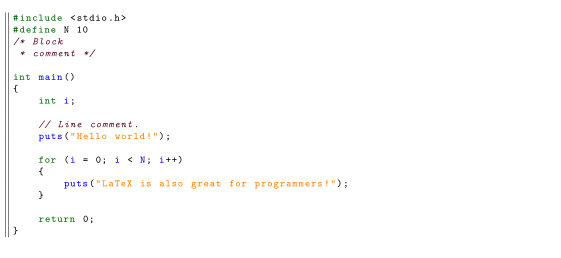
\includegraphics[width=0.50\textwidth]{gambar/contoh3}}
	\caption{Contoh Penggambaran}
	\label{contoh3}
\end{figure}

\begin{references}{Ham62}
\bibitem[Kil76]{kilb}J. S. Kilby,
``Invention of the Integrated Circuit,'' {\it IEEE Trans. Electron Devices,}
{\bf ED-23,} 648 (1976).

\bibitem[Ham62]{hamm}R. W. Hamming,
                 {\it Numerical Methods for Scientists and 
                 Engineers}, Chapter N-1, McGraw-Hill, 
                 New York, 1962.

\bibitem[Hu86]{lee}J. Lee, K. Mayaram, and C. Hu, ``A Theoretical
               Study of Gate/Drain Offset in LDD MOSFETs''
                     {\it IEEE Electron Device Lett.,} {\bf EDL-7}(3). 152 
                     (1986).

\bibitem[Ber87]{berm}A. Berenbaum, 
B. W. Colbry, D.R. Ditzel, R. D Freeman, and 
K.J. O'Connor, ``A Pipelined 32b Microprocessor with 13 kb of Cache Memory,''
{it Int. Solid State Circuit Conf., Dig. Tech. Pap.,} p. 34 (1987).

\end{references}



%%%%%%%%%%%%%%%
%%  The default LaTeX Index
%%  Don't need to add any commands before \begin{document}
\printindex

%%%% Making an index
%% 
%% 1. Make index entries, don't leave any spaces so that they
%% will be sorted correctly.
%% 
%% \index{term}
%% \index{term!subterm}
%% \index{term!subterm!subsubterm}
%% 
%% 2. Run LaTeX several times to produce <filename>.idx
%% 
%% 3. On command line, type  makeindx <filename> which
%% will produce <filename>.ind 
%% 
%% 4. Type \printindex to make the index appear in your book.
%% 
%% 5. If you would like to edit <filename>.ind 
%% you may do so. See docs.pdf for more information.
%% 
%%%%%%%%%%%%%%%%%%%%%%%%%%%%%%

%%%%%%%%%%%%%% Making Multiple Indices %%%%%%%%%%%%%%%%
%% 1. 
%% \usepackage{multind}
%% \makeindex{book}
%% \makeindex{authors}
%% \begin{document}
%% 
%% 2.
%% % add index terms to your book, ie,
%% \index{book}{A term to go to the topic index}
%% \index{authors}{Put this author in the author index}
%% 
%% \index{book}{Cows}
%% \index{book}{Cows!Jersey}
%% \index{book}{Cows!Jersey!Brown}
%% 
%% \index{author}{Douglas Adams}
%% \index{author}{Boethius}
%% \index{author}{Mark wain}
%% 
%% 3. On command line type 
%% makeindex topic 
%% makeindex authors
%% 
%% 4.
%% this is a Wiley command to make the indices print:
%% \multiprintindex{book}{Topic index}
%% \multiprintindex{authors}{Author index}

\end{document}

